\documentclass[12pt,letterpaper]{book}
\usepackage{mathptmx}
\usepackage{todonotes}
\usepackage[spanish,es-tabla]{babel}
\usepackage[latin1]{inputenc} 
\usepackage[T1]{fontenc}
\usepackage{amsmath}
\usepackage{amssymb, amsfonts, latexsym, cancel}
\usepackage{transparent}
\usepackage{eso-pic,graphicx}
\usepackage{epstopdf}
\usepackage{float}
\usepackage{subfigure}
\usepackage{array}
\usepackage[]{xcolor}
\usepackage[left=2cm,right=2cm,top=2cm,bottom=2cm]{geometry}
\usepackage{bm}
\usepackage[titletoc]{appendix}
\usepackage{subfigure}
\usepackage[subfigure]{tocloft}
\usepackage{multirow} % para las tablas
\usepackage{longtable}
\usepackage{lipsum}
\usepackage[breaklinks=true]{hyperref}
\usepackage[acronym,section=section]{glossaries}
\usepackage{fancyhdr, lastpage}
\usepackage{afterpage}
\usepackage{caption,newfloat}
%\usepackage{natbib}
\usepackage{apacite}
\usepackage{pdflscape}
\usepackage{titlesec}
\usepackage{enumerate} 
\usepackage{lipsum}  
\usepackage{listings, xcolor} 
\usepackage{siunitx}
%%%%%%%%%%%%%%%%%%%%%%%%%%%%%%%%%%%%%%%%%%%%%%%%%%
% Agregar una pagina en blanco
\newcommand\blankpage{%
    \null
    \thispagestyle{empty}%
    \addtocounter{page}{-1}%
    \newpage}
    

%%%%%%%%%%%%%%%%%%%%%%%%%%%%%%%%%%%%%%%%%%%%%%%%%%
% Modificacion de estilos de encabezados y pie de pagina
\fancypagestyle{plain}{
  \fancyhf{}% Clear header/footer
  \fancyfoot[R]{\thepage}% Right footer
  \renewcommand{\headrulewidth}{0.0pt}%
}
\pagestyle{plain}% Set page style to plain.
%%%%%%%%%%%%%%%%%%%%%%%%%%%%%%%%%%%%%%%%%%%%%%%%%%
% Modificar los niveles de nuemeracionº
\setcounter{secnumdepth}{6}
\setcounter{tocdepth}{3}
%%%%%%%%%%%%%%%%%%%%%%%%%%%%%%%%%%%%%%%%%%%%%%%%%%
% Modificacion de sangria
\parindent=0cm 
%%%%%%%%%%%%%%%%%%%%%%%%%%%%%%%%%%%%%%%%%%%%%%%%%%
% configuracion de anexos
\renewcommand{\appendixname}{Anexos}
\renewcommand{\appendixtocname}{Anexos}
\renewcommand{\appendixpagename}{Anexos}
%%%%%%%%%%%%%%%%%%%%%%%%%%%%%%%%%%%%%%%%%%%%%%%%%%
% Glosario correspondiente
% \gls{nombre} referenciar la palabra al glosario
% \acrfull{NOMBRE} referenciar el acronimo 
% \acrshort{NOMBRE} Escribir la descripcion del acronimo
% \newglossaryentry{nombre} 
% {
% name={Nombre},
% description={desc}
% }
 \newglossaryentry{grasa} 
 {
 name={grasa},
 description={tipo de nutriente que se obtiene en la alimentaci\'on, que le proporciona energ\'ia al cuerpo humano}
 }
 \newglossaryentry{condmet} 
 {
 name={condici\'on metab\'olica},
 description={Mide la capacidad de producir y consumir energ\'ia de un ser vivo}
 }
 \newglossaryentry{telem} 
 {
 name={telemetr\'ia},
 description={tecnolog\'ia que permite la medici\'on de magnitudes f\'isicas}
 }
 \newglossaryentry{diabetes} 
 {
 name={diabetes},
 description={Enfermedad que se origina debido que el p\'ancreas no sintetiza la cantidad de insulina que el cuerpo humano necesita.}
 }
 \newglossaryentry{rimeta} 
 {
 name={riesgos metab\'olico},
 description={conjunto de trastornos que aumenta el riesgo de padecer enfermedades card\'iacas, un derrame cerebral o diabet\'es.}
 }
 \newglossaryentry{asma} 
 {
 name={asma},
 description={enfermedad que afecta las v\'ias respiratorias debido al alto producci\'on de mucosa.}
 }
 \newglossaryentry{cancer} 
 {
 name={c\'ancer},
 description={Enfermedad en que una c\'elula se dividen sin control y destruyen los tejidos corporales}
 }
 \newglossaryentry{osteo} 
 {
 name={osteoporosis},
 description={Debilitaci\'on de los huesos. }
 }
  \newglossaryentry{infaef} 
 {
 name={infarto},
 description={bloqueo del flujo sangu\'ineo al coraz\'on}
 }
 \newglossaryentry{brad} 
 {
 name={base radial},
 description={procedimiento de redes neuronales, que calculan la salida en funci\'on de la distancia de un punto respecto a un punto central. }
 }
 
  \newglossaryentry{sigm} 
 {
 name={sigmoide},
 description={funci\'on matem\'atica, que se utiliza para suavizar los modelos de aprendizaje, cuya forma es de una S. }
 }
 
   \newglossaryentry{gaus} 
 {
 name={gaussiana},
 description={en t\'erminos de estad\'isticas, representa la distribuci\'on normal de un grupo de datos.}
 }
 
    \newglossaryentry{arbdec} 
 {
 name={\'arbol de decisi\'on},
 description={modelo de clasificador que se divide por distintos nodos de decisi\'on, para llegar a una respuesta (hoja).}
 }
 
    \newglossaryentry{knnia} 
 {
 name={K vecinos pr\'oximos},
 description={m\'etodo clasificador supervisado, que sirve para estimar la funci\'on de densidad respecto a un conjunto de datos cercanos al dato que se desea pronosticar}
 } 
 
     \newglossaryentry{redneu} 
 {
 name={red neuronal},
 description={paradigma de aprendizaje y procesamiento autom\'atico, cuya estructura esta formado por un sistema de interconexi\'on de neuronas que colaboran para producir una o varias salidas.}
 }
 
      \newglossaryentry{bayesian} 
 {
 name={clasificador bayesiano},
 description={clasificador probabil\'istico fundamento en el teorema de bayes (Probabilidad dado uno o m\'as eventos)}
 }
      \newglossaryentry{matcov} 
 {
 name={matriz de covarianza},
 description={matriz cuadrada que contiene las varianzas y covarianzas asociadas a diferentes variables}
 } 
      \newglossaryentry{elmia} 
 {
 name={m\'aquina de aprendizaje extremo},
 description={m\'aquina que se conforma de redes neuronales, cuya esencia es que la capa oculta de de la red se construye con un entrenamiento r\'apido y con poca participaci\'on humana}
 }  
       \newglossaryentry{svmia} 
 {
 name={m\'aquina de soporte vectorial},
 description={m\'etodo clasificador, la cual separa un conjunto de datos mediante un hiperplano de separaci\'on}
 }
 
  \newglossaryentry{Heur} 
 {
 name={heur\'istica},
 description={m\'etodo basado en la experiencia (informaci\'on previa), que puede utilizarse para resolver problemas }
 }


 
  \newglossaryentry{diseuc} 
 {	
 name={Distancia euclidiana},
 description={Distancia entre dos puntos}
 }
 
 
 \newglossaryentry{pixeles} 
 {
 name={pixeles},
 description={Unidades b\'asica de una imagen que obtiene el valor de un color}
 }
 
 \newglossaryentry{infrarrojo} 
 {
 name={infrarrojo},
 description={Radiaci\'on electromagn\'etica que emite un cuerpo, independiente a que exista otro tipo de luz}
 }
 
  \newglossaryentry{TOF} 
 {
 name={Tiempo de vuelo},
 description={T\'ecnica que se emplea para calcular distancia entre objetos}
 }
% \newacronym{NAME}{NAME}{DESCRIPCION}
\newacronym{TRESD}{3D}{tercera dimensi\'on}
\newacronym{RGBD}{RGB-D cameras}{c\'amaras con sensor de profundidad}
\newacronym{FPS}{FPS}{fotogramas por segundo}
\newacronym{FOV}{FOV}{campo de visi\'on}
\newacronym{NUI}{NUI}{interfaz de usuario natural}
\newacronym{SDK}{SDK}{Kit de desarrollo de software}
\newacronym{API}{API}{Interfaz de programación de aplicaciones}
\newacronym{LED}{LED}{Diodo de emisor de luz}
\newacronym{RAM}{RAM}{Memoria de acceso aleatorio}
\newacronym{XEF}{XEF}{extended event files}
\newacronym{RFR}{RFR}{Random Forest Regression}
\newacronym{AdaBoost}{AdaBoost}{Adaptive Boosting}
\newacronym{VGB}{VGB}{Visual Gesture Builder}
\makeglossaries
%%%%%%%%%%%%%%%%%%%%%%%%%%%%%%%%%%%%%%%%%%%%%%%%%%
% Definicion de ecuaaciones
\DeclareFloatingEnvironment[
  fileext=lofor,
  listname=Formula, % English name
  name=List of Formulas, % English name
  placement=tbp,
]{formula}

\addto\captionsspanish{% provide translations for Portuguese
  \renewcommand{\formulaname}{F\'ormula}%
  \renewcommand{\listformulaname}{\'Indice de f\'ormulas}%
}

%%%%%%%%%%%%%%%%%%%%%%%%%%%%%%%%%%%%%%%%%%%%%%%%%%
% Definicion de ecuaaciones
\DeclareFloatingEnvironment[
  fileext=loc,
  listname=Chart, % English name
  name=List of Charts, % English name
  placement=tbp,
]{chart}

\addto\captionsspanish{% provide translations for Portuguese
  \renewcommand{\chartname}{Gr\'afico}%
  \renewcommand{\listchartname}{\'Indice de Gr\'aficos}%
}
%%%%%%%%%%%%%%%%%%%%%%%%%%%%%%%%%%%%%%%%%%%%%%%%%%
% Definicion de codigo
\DeclareFloatingEnvironment[
  fileext=locode,
  listname=Code, % English name
  name=List of Codes, % English name
  placement=tbp,
]{code}

\addto\captionsspanish{% provide translations for Portuguese
  \renewcommand{\codename}{C\'odigo}%
  \renewcommand{\listcodename}{\'Indice de c\'odigos}%
}
%%%%%%%%%%%%%%%%%%%%%%%%%%%%%%%%%%%%%%%%%%%%%%%%%%
% Estilos de bibliografia
%\bibliographystyle{apalike} 
\bibliographystyle{apacite}
%%%%%%%%%%%%%%%%%%%%%%%%%%%%%%%%%%%%%%%%%%%%%%%%%%
% numeracion en letras para parrafos
\renewcommand{\theparagraph}{\Alph{paragraph}} 
\renewcommand{\thesubparagraph}{\Alph{paragraph}.\Alph{subparagraph}} 

\titleclass{\subsubparagraph}{straight}[\subparagraph]\newcounter{subsubparagraph}\renewcommand{\thesubsubparagraph}{\Alph{paragraph}.\Alph{subparagraph}.\Alph{subsubparagraph}} 
%%%%%%%%%%%%%%%%%%%%%%%%%%%%%%%%%%%%%%%%%%%%%%%%%%
% Configracion de codigo lstring
\lstset{
    string=[s]{"}{"},
    stringstyle=\color{gray},
    comment=[l]{:},
    commentstyle=\color{black},
    tabsize=2,
    frame=single
}
%%%%%%%%%%%%%%%%%%%%%%%%%%%%%%%%%%%%%%%%%%%%%%%%%%
\begin{document}
\frontmatter
\begin{titlepage}
\begin{center}
\AddToShipoutPictureBG*{\transparent{0.2}\includegraphics[width=\paperwidth,height=\paperheight]{graphics/logo.jpg}}
{\LARGE \textbf{UNIVERSIDAD RAFAEL LAND�VAR}}\\[0.1cm]
{\normalsize FACULTAD DE INGENIER�A}\\[0.1cm]
{\normalsize DEPARTAMENTO DE INGENIER�A EN INFORM�TICA Y SISTEMAS}\\[4cm]
{\huge \textbf{"M�quina de aprendizaje para la detecci�n de los pasos que se requiere para realizar un movimiento funcional mediante la utilizaci�n de una c�mara con sensor de profundidad"}}\\[0.1cm]
{\LARGE PROYECTO DE INGENIER�A}
\vfill
DIEGO JOS� ORELLANA BOJORQUEZ\\[0.1cm]
CARN� 10101-14\\[2cm]
Guatemala, Octubre de 2019\\[0.1cm]
Campus Central
\newpage
\end{center}
\end{titlepage}
\begin{center}
\AddToShipoutPictureBG*{\transparent{0.2}\includegraphics[width=\paperwidth,height=\paperheight]{graphics/logo.jpg}}
{\LARGE \textbf{UNIVERSIDAD RAFAEL LAND�VAR}}\\[0.1cm]
{\normalsize FACULTAD DE INGENIER�A}\\[0.1cm]
{\normalsize DEPARTAMENTO DE INGENIER�A EN INFORM�TICA Y SISTEMAS}\\[4cm]
{\huge \textbf{"M�quina de aprendizaje para la detecci�n de los pasos que se requiere para realizar un movimiento funcional mediante la utilizaci�n de una c�mara con sensor de profundidad"}}\\[0.1cm]
{\LARGE PROYECTO DE INGENIER�A}
\vfill
{\LARGE Presentada ante el Consejo de la Facultad de Ingenier�a}
\vfill
{\LARGE Por:}\\[0.1cm]
{\LARGE \textbf{DIEGO JOS� ORELLANA BOJORQUEZ}}
\vfill
Previo a optar el t�tulo de:\\[0.1cm]
Ingeniero en Inform�tica y Sistemas
\vfill
En el grado acad�mico de:\\[0.1cm]
Licenciado
\vfill
Guatemala, Octubre de 2019\\[0.1cm]
Campus Central
\end{center}
%%%%%%%%%%%%%%%%%%%%%%%%%%%%%%%%%%%%%%%%%%%%%%%%%
% notificaci�n
\afterpage{\blankpage}
\newpage
\includegraphics[width=18cm,height=22cm]{graphics/notificacion-tesis.jpg}
\afterpage{\blankpage}
\newpage
\includegraphics[width=18cm,height=22cm]{graphics/notificacion-tesis2.jpg}
%%%%%%%%%%%%%%%%%%%%%%%%%%%%%%%%%%%%%%%%%%%%%%%%%
\afterpage{\blankpage}
\newpage
{\LARGE \textbf{Agradecimientos}}\\[2cm]
\begin{itemize}
\item A Dios, por ser alguien que me escucha en todo momento.
\item A mi mam\'a, gracias a ella he llegado tan lejos, adem\'as de estar siempre conmigo en las buenas y en las malas. 
\item A mis hermanos, por tenerme paciencia y confiar en m\'i en todo momento.
\item A mi pap\'a, por acompa\~narme siempre.
\item A mis amigos de la universidad, por ser una gran promoci\'on unida y apoyarnos en todo momento.
\item A mis amigos del colegio, por mantener nuestra amistad y vernos crecer.
\item Ingenieros Stanly Bola\~nos y Victor Orozco, por apoyarme en todo el proceso de trabajo de investigaci\'on.
\item Departamento de deportes de la Universidad Rafael Land\'ivar, por confiar en mi proyecto de ingenier\'ia.
\end{itemize}
\begin{center}
Diego Orellana.
\end{center}
\newpage
\tableofcontents.
\listoffigures.
\listoftables.
\listofcharts.
\listofformulas.
\listofcodes.
\mainmatter
% mainmatter/
%index
\chapter{INTRODUCCI�N}
\lipsum[1-2]
\section{LO ESCRITO SOBRE EL TEMA}
\lipsum[1-2]
\section{MARCO TE�RICO}
\subsection{C\'AMARA CON SENSOR DE PROFUNDIDAD}
Los autores, \citeA{carfagni2017performance}, realizaron un estudio del rendimiento de la  c�mara, Intel SR300, en dicho estudio  se�alan las principales funciones de las \acrfull{RGBD}, entre ellas se puede mencionar la adquisici�n y procesamientos de datos en \acrfull{TRESD}, cabe mencionar que estas c�maras se han utilizado en el sector industrial y acad�mico (e.g. Reconocimiento de posiciones, gestos y objetos).
\medbreak
Por otro lado los autores, \citeA{henry2012rgb}, investigaron las variables necesarias para realizar un mapeo del ambiente (i.e. RGB-D mapping), cabe mencionar que las variables son analizado por medio de \gls{pixeles} de informaci�n de im�genes a color y de profundidad, tal como se muestra en la siguiente figura:
\begin{figure}[H]
	\caption{Captura de datos de una c\'mara con sensor de profundidad}
	\label{fig:RGBD}
	\centering
	\includegraphics[width=220px,height=50px]{graphics/RGB-D.PNG} \\
	\textbf{Fuente:} Tomado por el autor de tesis
\end{figure}
La figura \ref{fig:RGBD}, fue capturado por el dispositivo, Kinect de XBox One, a una velocidad de 28 \acrfull{FPS}, cabe mencionar que de lado izquierdo se tiene una vista a color, mientras que del lado derecho se tiene una vista de escala de grises (i.e. Datos de profundidad), por lo tanto en ambas im�genes se puede capturar distintas variables de an�lisis (e.g. Distancia, seguimiento, color, entre otras variables m�s...).
\subsubsection{Dispositivos en el mercado}
A continuaci�n se presentar� una lista de c�maras con sensor de profundidad, que se encuentra en el mercado hoy en d�a:
\begin{itemize}
	\item \textbf{ASUS XtionPro Live:} la corporaci�n, 	 ASUSTeK Computer \cite{xtionAsus}, desarroll� una c�mara con sensor de profundidad e infrarrojo, que permite detectar profundidad adaptativa, imagen a color y flujo de audio.
	\item \textbf{Structure Sensor:} La empresa, Occipital inc \cite{structureOccipital}, implement� un sensor de estructura, que permite escanear las personas, los espacios y los objetos en 3D. 
	\item \textbf{Intel RealSense cameras:} La empresa \citeA{intelRealSense}, desarroll� un producto de c�maras (i.e. Intel RealSense) que permite detectar una alta velocidad de cuadros (i.e. Frames por segundo), RGB de calidad y una resoluci�n de profundidad, cabe mencionar que estas c�maras se han utilizado en soluciones innovadoras (e.g. R�botica, drones, realidad virtual, entre otras aplicaciones m�s).
	\item \textbf{Microsoft Kinect:} El autor	\citeA{zhang2012microsoft}, realiz� un an�lisis de los componentes del Kinect, entre ellos se encuentra el sensor de profundidad, una c�mara a color y una matriz de micr�fonos que permite capturar movimientos, reconocer caracter�sticas faciales, construir un modelo del cuerpo en 3D y reconocer sonidos.
\end{itemize}
Tal como se observa en el listado, todas las c�maras con RGB-D tiene caracter�sticas similares que permite detectar elementos en el ambiente, sin embargo a la hora de escoger una c�mara se debe tomar en cuenta las siguientes especificaciones:
\begin{figure}[H]
	\caption{Especificaciones de una c\'amara con RGB-D}
	\label{fig:RGBESP}
	\centering
	\includegraphics[width=300px,height=170px]{graphics/RGBFeatures.png} \\
	\textbf{Fuente:} Tomado por el autor de tesis
\end{figure}
\medbreak
En la figura \ref{fig:RGBESP}, se muestra una vista general de las caracter�sticas de una c�mara con RGB-D, entre ellas se puede observar el alcance m�ximo de profundidad (i.e. Alcance del sensor 3D). As� mismo se encuentra el \acrfull{FOV}, cuya finalidad es determinar el �ngulo m�ximo de visi�n, respecto a los ejes: horizontal(H), vertical (V) y profundidad (D). Por otra parte, se encuentra la conexi�n de la c�mara al dispositivo, cuya funci�n es capturar los datos de entradas y salidas, como por ejemplo: la Resoluci�n de colores e infrarrojo (Tal como se observa en la figura \ref{fig:RGBD}).
\medbreak
A continuaci�n se presentar� una comparaci�n de las especificaciones entre las c�maras de RGB-D, mencionadas anteriormente:
\begin{table}[H]
\begin{center}
\caption{Comparaci�n de especificaciones entre c�maras de RGB-D }
\label{tab:RGBD}
\begin{tabular}{|l|l|l|l|l|l|} 
\hline
\textbf{Caracter�sticas}                                                          & \begin{tabular}[c]{@{}l@{}}\textbf{ASUS}\\\textbf{XtionPro}\\\textbf{Live}\end{tabular}   & \begin{tabular}[c]{@{}l@{}}\textbf{Structure}\\\textbf{Sensor}\end{tabular}  & \begin{tabular}[c]{@{}l@{}}\textbf{Intel}\\\textbf{RealSense}\\\textbf{SR300}\end{tabular}  & \begin{tabular}[c]{@{}l@{}}\textbf{Microsoft}\\\textbf{Kinect}\\\textbf{Live}\end{tabular} & \begin{tabular}[c]{@{}l@{}}\textbf{Microsoft}\\\textbf{Kinect}\\\textbf{v2}\end{tabular}	  \\ 
\hline
\begin{tabular}[c]{@{}l@{}}\textbf{Alcance del}\\\textbf{ sensor 3D}\end{tabular} & 0.8 a 3.5 m                                                                               & 0.4 a 3.5m                                                                   & 0.2 a 1.5m                                                                                  & 1.8 a 3.5m                                                                                 & 1.3 a 3.5m                                                                                  \\ 
\hline
\textbf{3D Resoluci�n}                                                            &\begin{tabular}[c]{@{}l@{}}640x480\\30fps\end{tabular}                   & \begin{tabular}[c]{@{}l@{}}640x480\\30fps\end{tabular}     & \begin{tabular}[c]{@{}l@{}}640x480\\60fps\end{tabular}                    &\begin{tabular}[c]{@{}l@{}}320x240\\30fps\end{tabular}					& \begin{tabular}[c]{@{}l@{}}512x424\\30fps\end{tabular}                    \\ 
\hline
\begin{tabular}[c]{@{}l@{}}\textbf{RGB}\\\textbf{ Resoluci�n}\end{tabular}        &\begin{tabular}[c]{@{}l@{}}1280x1024\\30fps\end{tabular}                   & \begin{tabular}[c]{@{}l@{}}640x480\\30fps\end{tabular}     & \begin{tabular}[c]{@{}l@{}}1920x1080\\30fps\end{tabular}                    &\begin{tabular}[c]{@{}l@{}}640x480\\30fps\end{tabular}					& \begin{tabular}[c]{@{}l@{}}1920x1080\\30fps\end{tabular}                    \\ 
\hline
\textbf{FOV}                                                                      & 58�H, 45�V                                                                                & 58�H, 45�V                                                                   & 73�H, 59�V                                                                                  & 57�H, 43�V                                                                                 & 70�H, 60�V                                                                                  \\ 
\hline
\textbf{Conexi�n}                                                                 & USB 2.0                                                                                   & USB 2.0                                                                      & USB 3.0                                                                                     & USB 2.0                                                                                    & USB 3.0                                                                                     \\
\hline
\end{tabular}
\end{center}
\textbf{Fuente:} Desarrollo de una aplicaci�n interactiva con Intel RealSense \cite{molero2018desarrollo} y Evaluation of the spatial resolution accuracy of the face tracking system for kinect for windows v1 and v2 \cite{amon2014evaluation}
\end{table}
\medbreak
En la tabla \ref{tab:RGBD}, se puede determinar que la c�maras: Intel RealSense SR300 y Microsoft Kinect V2, destacan de las dem�s c�maras, debido  que tiene una mayor resoluci�n del sensor RGB y un campo de visi�n m�s amplio, por lo cual para el presente proyecto se seleccionar� la c�mara Microsoft Kinect V2. 
\subsubsection{Microsoft Kinect V2}
En la gu�a de programaci�n de Kinect para Windows SDK \cite{jana2012kinect}, da a conocer caracter�stica del sensor Kinect, entre ellas se puede mencionar que el sensor Kinect se desarroll� para la consola de videojuegos, Xbox 360, adem�s proporciona una \acrfull{NUI}, que permite interactuar con el dispositivo a partir de movimientos, gestos y sonidos (i. e. Tecnolog�a con control de manos libres).
\medbreak
Por otra parte el autor, \citeA{jana2012kinect}, habla sobre el \acrfull{SDK}, cabe mencionar que dicho kit esta desarrollado para distintos lenguajes de programaci�n (e.g. C++, c\#, Python), sin embargo, para entender el funcionamiento del SDK se debe conocer la arquitectura del Kinect.
\\
\paragraph{Componentes}\mbox{} \\
\begin{figure}[H]
	\caption{Componentes del Kinect V2}
	\label{fig:COMPKINECT}
	\centering
	\includegraphics[width=400px,height=220px]{graphics/kinect-parts.PNG} \\
	\textbf{Fuente:} Tomado por el autor de tesis
\end{figure}
\medbreak
En la figura \ref{fig:COMPKINECT}, se muestra los componentes del Kinect que enlista el autor \citeA{jana2012kinect}, entre ellas se puede observar la c�mara a color cuya funci�n es capturar y transmitir los datos de v�deo en color, as� mismo se encuentra el sensor de profundidad conformado por el emisor de infrarrojo, que se encarga de escanear el ambiente constantemente  y convertirlo en informaci�n a partir del sensor de profundidad infrarroja (i.e. Identificaci�n de objetos), cabe mencionar que la c�mara puede rotar la imagen a partir de un peque�o motor que conecta la base y el cuerpo. Por otro lado, la matriz de micr�fonos permite capturar e identificar la direcci�n del sonido en el ambiente. Finalmente, se encuentra el  \acrfull{LED}, cuya tarea es identificar si los controladores del Kinect (e.g. IR, Seguimiento de objetos, RGB y sonido) est�n funcionando correctamente a partir de una luz blanca.
\paragraph{Conexi�n a la computadora}\mbox{} \\
\begin{figure}[H]
	\caption{Adaptador del Kinect V2}
	\label{fig:ADAPTERKINECT}
	\centering
	\includegraphics[width=400px,height=170px]{graphics/adapter-kinect.jpg} \\
	\textbf{Fuente:} \citeA{Kinectmanual}
\end{figure}
\medbreak
Tal como se observa en la figura \ref{fig:ADAPTERKINECT}, el cable de conexi�n esta conformado por 5 partes: (1) el cable de datos del Kinect que se encarga de recibir los datos de entradas y salidas del sensor, as� mismo esta (2) al adaptador del Kinect, que permite administrar los datos de entradas y salidas de la computadora y el sensor, a partir del (3) cable de USB 3. Cabe mencionar que dicho adaptador funciona con  un voltaje de 12 voltios y una corriente de 3 amperios que son administrado de una (4-5) fuente de alimentaci�n  que regula una entrada de 100 a 240 voltios y una corriente de 1.6 amperios.
\paragraph{Kit de desarrollo de Software (SDK)}\mbox{} \\
Para el presente proyecto se utilizar� el SDK de la empresa  \citeA{SDKKinect}, este SDK permite crear aplicaciones de reconocimientos de gestos y de voz con el sensor Kinect.
Cabe mencionar que para realizar estas aplicaciones, es necesario entender la interacci�n del software y del hardware:
\begin{figure}[H]
	\caption{Interacci�n del software y hardware}
	\label{fig:interaccionKinect}
	\centering
	\includegraphics[width=400px,height=180px]{graphics/interacionKinect.png} \\
	\textbf{Fuente:} Realizado por el autor de tesis
\end{figure}
En la figura \ref{fig:interaccionKinect}, se puede observar que el sensor kinect maneja 3 transmisiones de datos de salida:
\begin{itemize}
	\item \textbf{Datos de la imagen a color:} Seg�n el estudio de los c�digos de fuentes del SDK del Kinect \cite{hernandez2013analisis}, mencionan que los datos de imagen a color trabajan con un nivel de calidad que determina la velocidad en que los datos son transferidos (i.e. Frames por segundos), por otro lado permite conocer el formato en que se esta enviando dicha informaci�n: RGB (i.e. Mapa de bits a color de 32 bits) o YUV (i.e. Mapa de bits a color de 16 bits con correcci�n de transparencia de imagen).
	\item \textbf{Datos de c�mara de profundidad:} Los autores, \citeA{hernandez2013analisis}, mencionan que dicha transmisi�n esta conformada por el sensor de profundidad, cuya tarea es almacenar una escala de grises de todo el campo visible en un conjuto de p�xeles que representa una distancia de cercan�a con la c�mara (i.e. Base, altura y profundidad), cabe mencionar que la informaci�n es almacenado en 2 Bytes, la cual un Byte corresponde al emisor de IR y el otro Byte corresponde al sensor de profundidad IR.
	\item \textbf{Datos del sonido:} Seg�n el libro de detecci�n de movimiento y profundidad para NUI \cite{rahman2017beginning}, habla sobre la transmisi�n de sonido, dicha transmici�n captura el sonido en un rango m�ximo de 180 grados, as� mismo la informaci�n es almacenada en un vector de Byte (e.g. WAVEFORMAT, estructura b�sica de 16 Bytes).
\end{itemize}
Cabe mencionar que todas las transmisiones  interact�an a trav�s del recurso, NUI, dicho recurso esta compuesto por los siguientes elementos:
\begin{figure}[H]
	\caption{Arquitectura del Software, Kinect-NUI}
	\label{fig:architecturesSoftwareKinect}
	\centering
	\includegraphics[width=390px,height=300px]{graphics/kinect-software-architecture.PNG} \\
	\textbf{Fuente:} \cite[p.~14]{giori2013kinect}
\end{figure}
En el Libro, Kinect en  movimiento \cite{giori2013kinect}, dar a conocer los elementos que trabajan en el NUI (i.e. figura \ref{fig:interaccionKinect}):
\begin{enumerate}[1.]
    \item \textbf{Kinect Sensor:} Elemento que administra la conexi�n y los componentes del hardware.
    \item \textbf{Kinect Drivers:} Elemento que administra los drivers necesarios para el funcionamiento del Kinect (e.g. Audio, Arreglos de audio, c�maras, dispositivos y seguridad), cabe mencionar que dichos driver son accesible en el directorio:  \%Windows\%/System32/DriverStore/FileRepository, dentro de la carpeta "kinectsensor.inf".
    \item \textbf{NUI API:} Elemento que administra los componentes de SDK (i.e. Rastreo de esqueleto, audio, imagen de profundidad y de color), cabe mencionar que dichos componentes son accesible en el directorio: \%Archivos de programa\%/Microsoft SDKs/Kinect
    \item \textbf{DirectX Media Object (DMO):} Elementos que administra el funcionamiento de la matriz de audio (e.g. Identificar y analizar el origen de la fuente del audio).
    \item \textbf{Windows Standar API:} Elementos que administra los componentes complementarios del funcionamiento del sensor (e.g. Microsoft.speech, System.media, etc...).
\end{enumerate}
\subparagraph{Kinect v2 configuration verifier
}\mbox{} \\
Dicha aplicaci�n verifica y analiza el dispositivo que se encuentra conectado al sensor Kinect, tomando en cuenta las compatibilidades del hardware y la comunicaci�n del dispositivo al sensor:
\begin{figure}[H]
	\caption{Kinect v2 configuration verifier}
	\label{fig:KinectConfigurationVerifier}
	\centering
	\includegraphics[width=360px,height=300px]{graphics/kinect-configuration-verifier.PNG} \\
	\textbf{Fuente:} Tomado por el autor de tesis
\end{figure}
\medbreak
En la figura \ref{fig:KinectConfigurationVerifier}, se observa las siguientes validaciones:
\begin{itemize}
	\item \textbf{Update Configuration Definitions:} Verifica que tenga la �ltima versi�n del SDK (e.g. V.2).
		\item \textbf{Operating System:} Verifica si el sistema operativo es compatible (e.g. Windows 8 o superior).
		\item \textbf{Processor Cores:} Detecta si el procesador tiene los suficientes n�meros de core (e.g. Intel 5).
		\item \textbf{Physical Memory (RAM):} Chequea si el dispositivo tiene la suficiente memoria (e.g. M�nimo 4GB de RAM).
		\item \textbf{Graphics Processor:} Verifica si el procesador gr�fico es compatible con el SDK. (e.g. Directx 11).
		\item \textbf{USB Controller:} Verifica si el dispositivo reconoce el puerto de entrada (i.e. USB 3).	
		\item \textbf{Kinect Connected:} Detecta si el Sensor Kinect se encuentra conectado con el dispositivo.
		\item \textbf{Verify Kinect Software Installed:} Verifica las unidades (Drives) del sistema y el sensor.
		\item \textbf{Verify Kinect Depth and Color Streams:} Verifica los sensores de profundidad y de color (i.e. RGB e IR).
\end{itemize}
\subparagraph{Kinect Studio}\mbox{} \\
En el libro de detecci�n de movimiento y profundidad para NUI \cite{rahman2017beginning}, trabajan con algunas aplicaciones ya implementadas en el SDK, entre ellas se puede mencionar, Kinect Studio, aplicaci�n que permite capturar y reproducir datos del sensor en formato de v�deo, cabe mencionar que los datos son administrados por los siguientes monitores:
\begin{itemize}
	\item \textbf{Monitor NUI Body Frame:} Transmisi�n que contiene un espacio de almacenamiento para trabajar los datos de articulaciones del cuerpo.
	\item \textbf{Monitor NUI Body Index:} Transmisi�n que se encarga de clasificar y determinar los p�xeles de cada objeto.
	\item \textbf{Monitor NUI Depth:} Transmisi�n que se encarga de trabajar los datos de profundidad (i.e. Eje Z).
	\item \textbf{Monitor NUI IR:} Transmisi�n que trabaja con una imagen infrarroja a partir de la t�cnica de \gls{TOF}.
	\item \textbf{Monitor NUI Title Audio:} Transmisi�n que suministra el audio capturado en todas las direcciones.
	\item \textbf{Monitor NUI uncompressed color:} Transmisi�n encargada de proporcionar los datos de la imagen a color.	
\end{itemize}
Estos datos son almacenados en un archivo con formato, \acrfull{XEF}, dicho formato genera un v�deo de gran tama�o debido a la cantidad de datos que son capturados por los monitores, por lo cual se recomienda realizar varias repeticiones del movimiento en el menor tiempo posible y de igual manera capturar los siguientes datos para el an�lisis del movimiento:
\medbreak
\begin{figure}[H]
	\caption{Diagrama de Venn para la identificaci�n del movimiento de un objeto}
	\label{fig:VennStreaming}
	\centering
	\includegraphics[width=220px,height=150px]{graphics/venn-streaming.png} \\
	\textbf{Fuente:} Realizado por el autor de tesis
\end{figure}
\medbreak
En la figura \ref{fig:VennStreaming}, se puede observar que los monitores: Body index, Depth e IR, trabajan conjuntamente para reconocer los objetos, as� mismo es importante obtener datos correctos por medio de la calibraci�n de datos y tener disponible los datos en todo momento (i.e. Telemetr�a).
\medbreak
Finalmente en la figura \ref{fig:PlayKinectStudio}, puedes ver el resultado de un v�deo tomado por la aplicaci�n Kinect Studio, cabe mencionar que Kinect Studio te proporciona varias herramienta  para analizar el v�deo, tales como: el punto de Inicio y Fin, cuya funci�n es marcar una interacci�n (i.e. Segmento del v�deo), as� mismo puede indicar el n�mero de repeticiones de la interacci�n (i.e. cantidad de veces que desea ver el segmento del v�deo), adem�s de colocar puntos de pausa y etiquetas de metadatos, que te permitir� almacenar informaci�n adicional en un punto espec�fico del v�deo.
 \begin{figure}[H]
	\caption{Visualizaci�n del v�deo, Kinect Studio}
	\label{fig:PlayKinectStudio}
	\centering
	\includegraphics[width=400px,height=280px]{graphics/play-kinectstudio.png} \\
	\textbf{Fuente:} Tomado por el autor de tesis
\end{figure}
\subparagraph{Visual Gesture Builder}\mbox{} \\
El libro de detecci�n de movimiento y profundidad para NUI \cite{rahman2017beginning}, trabaja con una aplicaci�n de aprendizaje autom�tico llamada: \acrfull{VGB}, que permite crear una base de datos que reconocen los gestos en tiempo de ejecuci�n (Gesture DataBase, GDB), cabe mencionar que la herramienta utiliza dos algoritmos para la detecci�n de objetos, \acrfull{RFR} para modelos continuos, y \acrfull{AdaBoost} para modelos discretos. Se debe tomar en cuenta que los algoritmos analiza las siguientes variables en funci�n del tiempo:
\begin{itemize}
	\item Diferencia de posiciones.
	\item �ngulos de articulaciones y de movimientos.
	\item Velocidad de desplazamiento y angular.
	\item Aceleraci�n de desplazamiento y angular.	
	\item Fuerza muscular
	\item Torque muscular
\end{itemize}
Por lo que se refiere al modelo AdaBoost el autor, \citeA{AdaBoosting2018}, p�blica un art�culo cient�fico sobre la t�cnica de Boosting, en la cual consta en mejorar las predicciones del modelo, a partir de un n�mero de entrenamientos secuenciales, tal como se observa la siguiente figura:
\begin{figure}[H]
	\caption{T�cnica Boosting}
	\label{fig:AdaBoost}
	\centering
	\includegraphics[width=400px,height=200px]{graphics/AdaBoosting.png} \\
	\textbf{Fuente:} Realizado por el autor de tesis
\end{figure}
\medbreak
En la figura \ref{fig:AdaBoost}, se observa que en el entrenamiento \# 1,  los datos de entradas se encuentra muy dispersos, por lo tanto, cada dato de entrada se  debe entrenar a partir de un algoritmo de aprendizaje, que permitir� transformar una nueva funci�n, tal como se observa el entrenamiento \# 2, los datos de entradas est�n m�s cercano. Cabe mencionar que se debe establecer los n�meros de entrenamientos y el algoritmo de aprendizaje que utilizar� por cada entrenamiento, siguiendo con el ejemplo de la figura \ref{fig:AdaBoost}, tiene un total de 2 entrenamientos, y cada entrenamiento consta de operar el dato de entrada por su respectiva regresi�n lineal y una constante.
\medbreak
Cabe mencionar que el modelo discreto, es recomendable utilizarlo para identificar movimientos est�ticos (e.g. Identificar si la persona se encuentra sentada, arrodillada, entre otros movimientos m�s...), por lo que el software, VGB, permite analizar el v�deo (i.e. xef) y posteriormente etiquetar los momentos que se encuentra realizando dicho movimientos est�ticos:
\begin{figure}[H]
	\caption{Etiquetas de movimientos est�tico}
	\label{fig:modeloDiscreto}
	\centering
	\includegraphics[width=400px,height=350px]{graphics/modelo-discreto.png} \\
	\textbf{Fuente:} Realizado por el autor de tesis
\end{figure}
\medbreak
En la figura \ref{fig:modeloDiscreto}, se puede observar que en el panel de control puede etiquetar los valores: positivos (Barra azul arriba) y negativos (Barra azul abajo), as� mismo se observa el movimiento est�tico, Manos abajo, que consta en identificar que ambas manos y brazos est�n tocando la parte dorsal del cuerpo (i.e. Figura \ref{fig:modeloDiscreto}.B), en caso que este realizando otro movimiento, el valor de la etiqueta ser� falso (i.e.  Figura \ref{fig:modeloDiscreto}.C).
\medbreak
Por lo que se refiere al modelo Random Forest Regression, la autora, \citeA{RandomForestRegression2018} realiz� un art�culo cient�fico sobre este modelo, en donde indica que es un algoritmo de var�as t�cnicas de predicciones (i.e. regresiones y �rboles de decisiones),cabe mencionar que el entrenamiento se basa en la t�cnica llamada, Boostrap Aggregation, que consta en entrenar cada �rbol de decisi�n a partir de las variables de an�lisis, tal como se observa en la figura \ref{fig:RandomForestRegression}:
\begin{figure}[H]
	\caption{T�cnica Random Forest Regression}
	\label{fig:RandomForestRegression}
	\centering
	\includegraphics[width=400px,height=170px]{graphics/random-forest-regression.png} \\
	\textbf{Fuente:} Realizado por el autor de tesis
\end{figure}
\medbreak
Finalmente, el modelo continuo es recomendable utilizarlo para identificar movimientos din�micos (e.g. Sentadillas, abdominales, saltos, entre otros movimientos m�s...), tal como se observa en la siguiente figura:
\begin{figure}[H]
	\caption{Etiquetas de movimientos din�micos}
	\label{fig:modeloContinuo}
	\centering
	\includegraphics[width=400px,height=250px]{graphics/modelo-continuo.png} \\
	\textbf{Fuente:} Realizado por el autor de tesis
\end{figure}
En la figura \ref{fig:modeloContinuo}, se esta analizando el movimiento de vuelo, la cual se conforma de tres movimientos est�ticos: Brazos abajos (i.e. Figura \ref{fig:modeloContinuo}.B), brazos al medio (i.e. Figura \ref{fig:modeloContinuo}.C)  y brazos arriba (i.e. Figura \ref{fig:modeloContinuo}.D),  por lo tanto para analizar y detectar el movimiento din�mico, se etiqueta con un valor decimal a cada movimiento est�tico, tal como se observa en la figura, el primer paso del movimiento din�mico esta entre el valor de 0.00 a 0.33. 
\subparagraph{Skeletal Tracking}\mbox{} \\
En el an�lisis y estudio de los c�digo de fuente de SDK del Kinect \cite{hernandez2013analisis}, los autores realizaron un an�lisis del seguimiento del esqueleto, en la cual observaron que genera la figura humana a trav�s de 25 puntos que representa las principales articulaciones del cuerpo, tal como se muestra en la figura \ref{fig:jointsKinect}:
\begin{figure}[H]
	\caption{Seguimiento de uniones del Kinect}
	\label{fig:jointsKinect}
	\centering
	\includegraphics[width=360px,height=450px]{graphics/jointKinect.png} \\
	\textbf{Fuente:} \cite[]{rocha2015kinect}
\end{figure}
As� mismo los autores, \citeA{hernandez2013analisis}, indican que el seguimiento del esqueleto asocia los par�metros del cuerpo humano (e.g. Extremidades superiores, articulaciones, gestos...), dichos par�metros son utilizado por un SkeletonFrame, cuya finalidad es reconocer el borde del cuerpo humano y posteriormente reconocer cada parte del esqueleto humano, a partir del SkeletonData, tal como se muestra en la figura \ref{fig:skeletanTracking}:
\begin{figure}[H]
	\caption{Arquitectura del seguimiento del esqueleto}
	\label{fig:skeletanTracking}
	\centering
	\includegraphics[width=450px,height=200px]{graphics/SkeletanTracking.png} \\
	\textbf{Fuente:} Elaborado por el autor de tesis
\end{figure}
En la figura \ref{fig:skeletanTracking} se observa que el seguimiento de esqueleto esta conformado por 6 pasos: (1) como primer paso el Kinect escanea el ambiente constantemente, (2) posteriormente se crea el mapa de profundidad,(3) esto permitir�  detectar el suelo y separar los objetos, con el fin de objetivo de identificar el contorno humano de cada jugador, (4) luego por cada jugador se le asigna un identificador y clasifica las partes del cuerpo humano (e.g. Cabeza, brazos, manos, piernas, etc...), (5) seguidamente a cada parte del cuerpo humano se le asigna una uni�n  y (6) finalmente unifica cada uni�n en el orden correspondiente, tal como se observa en la figura \ref{fig:jointsKinect}.
\medbreak
En cuanto las uniones (Joints), los autores,  \citeA{hernandez2013analisis}, menciona que cada uni�n se encuentra en un sistema diestro de coordenada en donde cada eje (i.e. X, Y, Z) representa la distancia (En metros) del Kinect al Joint, tal como se representa en la figura \ref{fig:CoordenadaJoint}:
\begin{figure}[H]
	\caption{Sistema de coordenada de la uni�n (Joint)}
	\label{fig:CoordenadaJoint}
	\centering
	\includegraphics[width=450px,height=190px]{graphics/PartsToJoin.png} \\
	\textbf{Fuente:} Elaborado por el autor de tesis
\end{figure}
\chapter{Planteamiento del problema}
Dentro del \'area deportiva, las personas realizan entrenamiento de alta intensidad de un movimiento, con el fin objetivo de mejorar las habilidades f\'isicas. Sin embargo, al momento de que una persona est\'a realizando un movimiento, se est\'a desarrollando su coordinaci\'on (habilidad f\'isica), la cual consta en combinar varios pasos de manera ordenada para ejecutar el movimiento, sin embargo esta habilidad f\'isica puede llegar a presentar 2 problemas:
\begin{itemize}
	\item El primer problema consta de un usuario nuevo que desconoce como ejecutar el movimiento.
	\item El segundo problema se compone de un usuario que conoce el movimiento, pero lo ejecuta de distinta manera.
\end{itemize} 
La primera problem\'atica se resuelve si los atletas y los entrenadores le ense\~nan al nuevo usuario los pasos requeridos para ejecutar un movimiento v\'alido, con la finalidad de que el nuevo usuario lo aprenda y lo entrene constantemente.
\medbreak
El segundo problema surge cuando el usuario cambia de lugar de entrenamiento, debido que puede presentar nuevos criterios para ejecutar los movimientos que ha aprendido hacer, y esto puede conllevar a crear una discusi\'on: ?`Es v\'alido el movimiento que se conoce?
\medbreak
\medbreak
As\'i mismo el segundo problema se ha encontrado en eventos deportivos en Guatemala, por ejemplo el evento Unleash Your Fitness \cite{unleash}, competencia que presenta la modalidad de conteos de repeticiones de movimientos, en donde ha surgido conflictos de contabilizaciones de repeticiones de  movimientos v\'alidos entre jueces y atletas.
\medbreak
\medbreak
En resumen, el presente proyecto implementa la tecnolog\'ia de Visual Gesture Builder (etiquetador de fotogramas del seguimiento del esqueleto) con la finalidad de aplicar el algoritmo Random Forest Regression, para determinar la coordinaci\'on en un valor num\'erico llamado factor del movimiento y al mismo tiempo responder la siguiente pregunta:
\medbreak
\medbreak
\begin{center}
\textbf{?`Es posible clasificar el movimiento de una persona durante una actividad f\'isica como v\'alido o inv\'alido?}
\end{center}
\section{Objetivos}
\subsection{Objetivo general}
Implementar un algoritmo clasificador de movimiento v\'alido o inv\'alido a partir del modelo de  detecci�n de los pasos requeridos del movimiento,  con la ayuda del algoritmo de Random Forest Regression y la utilizaci\'on del dispositivo Kinect V2.
\subsection{Objetivos espec\'ificos}
\begin{enumerate}[1.]
\item Definir el movimiento a analizar, estableciendo los pasos requeridos para realizar un movimiento v\'alido.
\item Grabar los v\'ideos de atletas realizando repeticiones del movimiento v\'alido a partir de la herramienta, Kinect studio.
\item Crear el modelo de detecci\'on de los pasos requeridos de un movimiento v\'alido, aplicando el algoritmo de Random Forest Regression y la etiquetaci\'on de fotogramas de los v\'ideos.
\item Crear un algoritmo clasificador que clasifique la repetici\'on de un movimiento v\'alido.
\end{enumerate}
\section{HIP�TESIS}
M\'etodo indirecto que eval\'ua la condici\'on metab\'olica de una persona al momento de realizar un entrenamiento interv\'alado con movimientos funcionales.
\section{VARIABLES} \label{vr}
\subsection{VARIABLES DEPENDIENTES} \label{vr:d}
\begin{enumerate}
   \item[A.] Entorno
   \begin{enumerate}
       \item[A.A.] Distancia m\'inima de profundidad entre la persona y el Kinect -i.e. Eje z-.
       \item[A.B.] Distancia m\'axima de profundidad entre la persona y el Kinect -i.e. Eje z-.
   \end{enumerate}
   \item[B.] Kinect
   \begin{enumerate}
      \item[B.A] Articulaciones
       \begin{enumerate}
	       \item[B.A.A.] Horizontal -i.e. Eje x-.
       	   \item[B.A.B.] Vertical -i.e. Eje y-.
       \end{enumerate}
       \item[B.B] Tiempo de captura de la imagen.
   \end{enumerate}
   \item[C.] Habilidades f\'isicas
   \begin{enumerate}
   		\item[C.A.] Flexibilidad.
   		\begin{enumerate}
   			\item[C.A.A.] \'Angulo de movimiento por articulaci\'on.
   		\end{enumerate}
   \end{enumerate}  
   \item[D.] Actividad F\'isica
   \begin{enumerate}   		
   		\item[D.A.] Series de movimientos funcionales.
   	    \item[D.B.] Repeticiones de movimientos funcionales.
   	    \item[D.C.] Entrenamiento Interval\'ado  controlado-
   	    \begin{enumerate}
   	    	\item[D.C.A.] Tiempo de descanso.
   	    	\item[D.C.B.] Tiempo de trabajo.
   	    \end{enumerate}  
   \end{enumerate}  
\end{enumerate}
\subsubsection{Definici\'on de variables dependientes}
\begin{table}[H]
\begin{center}
\caption{Descripci\'on operacional y conceptual de las variables dependientes}
\label{tab:defVarDep}
\begin{tabular}{|c|l|l|}
\hline
\textbf{Enumeracion} & \multicolumn{1}{c|}{\textbf{Definicion operacional}} & \multicolumn{1}{c|}{\textbf{Definicion conceptual}} \\ \hline
\ref{vr:d}.A.A. & \begin{tabular}[c]{@{}l@{}}Distancia de profudidad \\ m\'inima en metros, la cual el Kinect \\ puede detectar correctamente el \\ seguimiento de esqueleto de una persona,\\ para realizar un movimiento funcional.\end{tabular} & \multirow{2}{*}{\begin{tabular}[c]{@{}l@{}}De acuerdo a la secci\'on \ref{mt:cam:mer},\\ dicha distancia \\ es calculada a partir del\\ alcance del sensor 3D de\\ una c\'amara con RGB-D.\\ As\'i mismo el valor esta\\ comprendido entre 1.3 a\\ 3.5 metros (ver Tabla \ref{tab:RGBD}).\end{tabular}} \\ \cline{1-2}
\ref{vr:d}.A.B. & \begin{tabular}[c]{@{}l@{}}Distancia de profudidad \\ m\'axima en metros, la cual el Kinect \\ puede detectar correctamente el \\ seguimiento de esqueleto de una persona,\\ para realizar un movimiento funcional.\end{tabular} &  \\ \hline
\ref{vr:d}.B.A.A. & \begin{tabular}[c]{@{}l@{}}Distancia horizontal en p\'ixeles, entre\\ el Kinect y una articulaci\'on de una \\ persona.\\ \\ \\ \\ \end{tabular} & \multirow{2}{*}{\begin{tabular}[c]{@{}l@{}}Seg\'un la secci\'on \ref{mt:cam:kin}.\ref{mt:cam:kin:st},\\ cada articulaci\'on del \\ esqueleto esta dado por el \\ Skeleton Data, la cual es \\ mapeado por un espacio de\\ profundidad, para describir\\ la ubicaci\'on en 2D -i.e \\ Altura y anchura- por medio\\ del Skeleton Frame (ver \\ Figura  \ref{fig:skeletanTracking}).\end{tabular}} \\ \cline{1-2}
\ref{vr:d}.B.A.B. & \begin{tabular}[c]{@{}l@{}}Distancia vertical en p\'ixeles, entre\\ el Kinect y una articulaci\'on de una \\ persona. \\ \\ \\ \\ \\ \end{tabular} &  \\ \hline
\ref{vr:d}.B.B. & \begin{tabular}[c]{@{}l@{}}Tiempo en segundos,  en donde el Kinect\\ dibuja los frames del seguimiento del\\ esqueleto -i.e. 0.017 \\ segundos por frame-.\end{tabular} & \begin{tabular}[c]{@{}l@{}}Concorde a la secci\'on \ref{mt:cam:kin}.\ref{mt:cam:kin:ks},\\ el seguimiento de esqueleto son\\ necesarios los NUIs de: Profundidad\\ e infrarroja (ver Figura \ref{fig:VennStreaming}). Por\\ lo tanto el seguimiento de esqueleto\\ corre a 60 fps  -i.e. 30 fps de \\ resoluci\'on de 3D y 30 fps de \\ resoluci\'on  RGB-. (ver Tabla \ref{tab:RGBD}).\end{tabular} \\ \hline
\end{tabular}
\end{center}
\textbf{Fuente:} Elaborada por el autor de tesis
\end{table}
\begin{table}[H]
\begin{center}
\caption{Continuacion Descripci\'on operacional y conceptual de las variables dependientes}
\label{tab:defVarDep2}
\begin{tabular}{|c|l|l|}
\hline
\textbf{Enumeracion} & \multicolumn{1}{c|}{\textbf{Definicion operacional}} & \multicolumn{1}{c|}{\textbf{Definicion conceptual}} \\ \hline
\ref{vr:d}.C.A.A. & \begin{tabular}[c]{@{}l@{}}\'Angulo en grado sexagesimal, que \\ determina el arco de movimiento de \\ cada articulacion del cuerpo humano.\end{tabular} & \begin{tabular}[c]{@{}l@{}}Conforme a la seccion \ref{mt:mf:var} la,\\ flexibilidad mide el rango del\\ movimiento muscular, de\\ acuerdo a los arcos de movilidad \\ del cuerpo humano\\ (ver figuras: \ref{fig:ArcosdeMovilidad} y \ref{fig:ArcosdeMovilidad2}).\end{tabular} \\ \hline
\ref{vr:d}.D.A. & \begin{tabular}[c]{@{}l@{}}Unidad que mide las repeticiones de\\ un movimiento de funcional . \\ \\ \\ \\\end{tabular} & \multirow{2}{*}{\begin{tabular}[c]{@{}l@{}}De acuerdo a la secci\'on \ref{mt:af:var}, al \\ momento de realizar actividad f\'isica,\\ la persona realiza ciertas cantidades \\ de series de movimientos f\'isico,\\ conformado por una cantidad de \\ repeticiones -i.e.  movimientos \\ repetitivos-.\end{tabular}} \\ \cline{1-2}
\ref{vr:d}.D.B. & \begin{tabular}[c]{@{}l@{}}Unidad que mide el lapso del\\ paso inicial y final de un movimiento\\ funcional, de manera repetitiva. \\ \\ \end{tabular} &  \\ \hline
\ref{vr:d}.D.C.A. & \begin{tabular}[c]{@{}l@{}}Tiempo en segundos,  la cual pausa\\ la actividad de seguimiento esqueleto. \\ \\ \end{tabular} & \multirow{2}{*}{\begin{tabular}[c]{@{}l@{}}Segun la secci\'on \ref{mt:mf:rut}.\ref{mt:mf:rut:hiit}, estas\\ variables son necesarias para realizar\\ el entrenamiento intervalado \\ controlado, tabata. En donde el tiempo\\ de trabajo debe ser mayor o igual al \\ tiempo de descanso.\end{tabular}} \\ \cline{1-2}
\ref{vr:d}.D.C.B & \begin{tabular}[c]{@{}l@{}}Tiempo en segundos, la cual esta \\ activo la actividad del seguimiento del\\ esqueleto \\ \\.\end{tabular} &  \\ \hline
\end{tabular}
\end{center}
\textbf{Fuente:} Elaborada por el autor de tesis
\end{table}
\subsection{VARIABLES INDEPENDIENTES}
\begin{enumerate}
   \item[A.] Entorno
    \begin{enumerate}
       \item[A.A.] Altura del Kinect -i.e. Eje y-
       \item[A.B.] Punto de an\'alisis -i.e. Centro de equilibrio-.
   \end{enumerate}
   \item[B.] Habilidades f\'isicas
   \begin{enumerate}
   		\item[B.A.] Precisi\'on.
   		\begin{enumerate}
   			\item[B.A.A] Clasificaci\'on por cada paso del movimiento funcional -i.e. Correcto o incorrecto-.
   		\end{enumerate}
   		\item[B.B.] Velocidad.
   		\begin{enumerate}
   			\item[B.B.A.] Tiempo por repetici\'on.
   			\item[B.B.B.] Tiempo por serie.
   		\end{enumerate}
   		\item[B.C.] Agilidad.
   		\begin{enumerate}
   			\item[B.C.A] Tiempo por cada paso del movimiento funcional.
   		\end{enumerate}
   		\item[B.D.] Potencia.
   		\begin{enumerate}
   			\item[B.D.A] Cantidad m\'axima de series por repetici\'on.
   		\end{enumerate}
  \end{enumerate}
  \item[C.] Visual Gesture Builder
  \begin{enumerate}
  	\item[C.A.] Factor discreto.
  	\item[C.A.] Factor continuo.
  \end{enumerate}
\end{enumerate}

\section{ALCANCES Y L\'IMITES}
\section{Aportes}
El presente proyecto aporta un software que identifica si una persona esta en movimiento, con la ayuda de dos \'areas de estudios:
\begin{itemize}
	\item \textbf{Visi\'on artificial:} La investigaci\'on brinda informaci\'on sobre el funcionamiento del sensor Kinect y sus respectivas herramientas, las cuales ayudan a crear una base de datos de reconocimiento de gesturas y posturas, usando la tecnolog\'ia de m\'aquinas de aprendizajes -i.e. Bosques de regresiones aleatorias-, con la finalidad de crear un modelo que detecta el movimiento de una persona.
	\item \textbf{Salud y deporte para el control del sedentarismo:} La investigaci\'on aporta tres movimientos que se pueden ejecutar en rutinas de alta intensidad, que permiten estimular el cuerpo humano para cumplir las recomendaciones de la Organizaci\'on Mundial de la Salud.
\end{itemize}

\chapter{M�TODO}
\section{Sujetos}
El departamento de deportes de la Universidad Rafael Land\'ivar, le proporcion\'o al investigador, la colaboraci\'on de todos los deportes -e.g. F\'utbol, voleibol, baloncesto, tenis, banda, zumba, atletismo, nataci\'on, taekwondo, tenis de mesa y animaci\'on-. Lo cual el investigador tuvo que realizar filtros para seleccionar la poblaci\'on, descartando aquellos deportes que entrenaban en las federaciones nacionales de Guatemala -i.e. Lugares externos a la Universidad Rafael Land\'ivar-, entre ellos estaban: Atletismo, nataci\'on y tenis. Por otro lado, el investigador apart\'o los deportes que se ejercitaban dentro de una cancha deportiva debido a la dificultad de colocar todos los materiales necesarios del proyecto para la toma de datos, por lo cual se elimin\'o los deportes de:  f\'utbol, voleibol y baloncesto. Finalmente, el investigador ignor\'o los deportes de banda y zumba, ya que son actividades que se trabajan en conjunto con otros departamentos de la Universidad Rafael Landivar -e.g. Unidad de artes Land\'ivar-. De modo que el investigador seleccion\'o los siguientes deportes:
\begin{itemize}
	\item \textbf{Tenis de mesa:} Deporte de raqueta que se juega sobre una mesa rectangular de manera individual o en parejas, con el fin objetivo de golpear una peque\~na pelota.
	\item \textbf{Animaci\'on:} Deporte grupal que combina la m\'usica y gimnasia, a partir de rutinas de baile que entusiasma un p\'ublico o evento deportivo.
	\item \textbf{Taekwondo:} Deporte individual basado en el arte marcial coreano moderno, que consiste en el uso de los pies, brazos y pu\~nos dentro de un combate.
\end{itemize}
\subsection{Primer tipo} \label{sj:1t}
Define la cantidad de sujetos que participaron en la colecta de los datos para la creaci\'on del modelo de reconocimiento del movimiento, a partir de tres fases distintas:
\begin{itemize}
	\item \textbf{Construcci\'on:} Atletas que construyeron el modelo continuo de la m\'aquina de aprendizaje.
	\item \textbf{Pruebas:} Muestra de usuarios que se emple\'o para el c\'alculo de los m\'argenes de  errores del pron\'ostico del modelo.
	\item \textbf{Validaci\'on:} Conjunto de deportistas que realizaron las pruebas al modelo en tiempo real.
\end{itemize}
\subsubsection{Equipo de animaci\'on de la Universidad Rafael Land\'ivar} \label{sj:1t:ani}
\begin{table}[H]
\begin{center}
\caption{Muestra del equipo de animadoras}
\label{tab:MuestraCheerleaders}
\begin{tabular}{lc}
\hline
\multicolumn{1}{|l|}{\textbf{Descripci\'on}} & \multicolumn{1}{l|}{\textbf{Cantidad}} \\ \hline
\multicolumn{1}{|l|}{Atletas para la construcci\'on del modelo} & \multicolumn{1}{c|}{6} \\ \hline
\multicolumn{1}{|l|}{Atletas para las pruebas del modelo} & \multicolumn{1}{c|}{1} \\ \hline
\multicolumn{1}{|l|}{Atletas para la validaci\'on del modelo} & \multicolumn{1}{c|}{2} \\ \hline
\multicolumn{1}{|r|}{Total de atletas} & \multicolumn{1}{c|}{9} \\ \hline
\textbf{Fuente:} Observaci\'on del investigador durante el trabajo de campo.
\end{tabular}
\end{center}
\end{table}
\subsubsection{Equipo de tenis de mesa de la Universidad Rafael Land\'ivar}\label{sj:1t:ten}
\begin{table}[H]
\begin{center}
\caption{Muestra del equipo de tenis de mesa}
\label{tab:MuestraTenis}
\begin{tabular}{lc}
\hline
\multicolumn{1}{|l|}{\textbf{Descripci\'on}} & \multicolumn{1}{l|}{\textbf{Cantidad}} \\ \hline
\multicolumn{1}{|l|}{Atletas para la construcci\'on del modelo} & \multicolumn{1}{c|}{5} \\ \hline
\multicolumn{1}{|l|}{Atletas para las pruebas del modelo} & \multicolumn{1}{c|}{1} \\ \hline
\multicolumn{1}{|l|}{Atletas para la validaci\'on del modelo} & \multicolumn{1}{c|}{3} \\ \hline
\multicolumn{1}{|r|}{Total de atletas} & \multicolumn{1}{c|}{9} \\ \hline
\textbf{Fuente:} Observaci\'on del investigador durante el trabajo de campo.
\end{tabular}
\end{center}
\end{table}
\subsubsection{Equipo de taekwondo de la Universidad Rafael Land\'ivar}\label{sj:1t:tae}
\begin{table}[H]
\begin{center}
\caption{Muestra del equipo de taekwondo}
\label{tab:MuestraTaekwondo}
\begin{tabular}{lc}
\hline
\multicolumn{1}{|l|}{\textbf{Descripci\'on}} & \multicolumn{1}{l|}{\textbf{Cantidad}} \\ \hline
\multicolumn{1}{|l|}{Atletas para la construcci\'on del modelo} & \multicolumn{1}{c|}{13} \\ \hline
\multicolumn{1}{|l|}{Atletas para las pruebas del modelo} & \multicolumn{1}{c|}{1} \\ \hline
\multicolumn{1}{|r|}{Total de atletas} & \multicolumn{1}{c|}{14} \\ \hline
\textbf{Fuente:} Observaci\'on del investigador durante el trabajo de campo.
\end{tabular}
\end{center}
\end{table}
\subsection{Segundo tipo} \label{sj:2t}
A continuaci\'on se muestra un organigrama de la estructura del departamento de deportes de la Universidad Rafael Land\'ivar, en ella se muestra todos los profesionales que aportaron en la investigaci\'on:
\begin{figure}[H]
	\caption{Organigrama del departamento de deportes de la Universidad Rafael Land\'ivar}
	\label{fig:orgDeportes}
	\centering
	\includegraphics[width=450px,height=170px]{graphics/orgDeportes.png} \\
	\textbf{Fuente:} Elaborado por el autor de tesis
\end{figure}
\subsection{Unidades de an\'alisis} \label{sj:ua}
Para el presente proyecto se utiliz\'o como referencia el manual de acondicionamiento de fuerza y prevenci\'on de lesiones  \cite{arbour2006strength}, la cual describe los movimientos ideales para el calentamiento  y estiramiento de una rutina. (Ver secci\'on de anexos \ref{anx:warmup}).
\input{mainmatter/metodo/unidades-de-analisis}
\section{Instrumentos}\label{ins}
El conjunto de instrumentos se elabor\'o con los  siguientes recursos:
\begin{itemize}
\item Humanos
	\begin{itemize}
	\item Profesionales -i.e. Entrenadores-.
	\item Atletas
	\item Investigador
	\end{itemize}
\item No humanos
	\begin{itemize}
	\item Mesa de soporte con una altura de 0.70 metros.
	\item Cable de extensi\'on el\'ectrico de 2.00 metros. 
	\item Computadora port\'atil
		\begin{itemize}
		\item Conector de carga de alimentaci\'on
		\end{itemize}
	\item Sensor Kinect
		\begin{itemize}
		\item Adaptador del Kinect
		\end{itemize}
	\end{itemize}
\end{itemize}
\subsection{Formulario de registro de movimiento} \label{ins:frmMov}
Este formulario se adjunta en anexos (ver figura \ref{fig:frmWhiteMov}), la cual tiene como objetivo describir el movimiento de cada equipo deportivo. Por otra parte, el formulario est\'a compuesto por los siguientes incisos:
\begin{itemize}
	\item \textbf{Nombre del movimiento:} Nombre que se identifica en gu\'ias deportivas o de salud.
	\item \textbf{Descripci\'on del movimiento: } Contesta la pregunta: ?`Qu\'e es el movimiento?
	\item \textbf{Movimiento unilateral:} Si es afirmativo, el movimiento trabaja con solo una parte del cuerpo (izquierda o derecha, ejemplo una patada), en caso contrario, se considera todas las partes del cuerpo (izquierda y derecha, ejemplo un salto).
	\item \textbf{Partes del cuerpo ignorada:} M\'ultiples respuestas que identifican las articulaciones ignoradas -i.e. Debido que no es informaci\'on relevante para el movimiento-:
	\begin{itemize}
		\item \textbf{Brazo derecho o izquierdo:} Ignora las siguientes articulaciones (seg\'un su lado): Pulgar, dedo del medio, mano, codo, hombro, centro de los hombros, cuello, cabeza y espalda.
		\item \textbf{Cuerpo inferior:} Ignora las siguientes articulaciones (en ambos lados): Centro de cadera, caderas, rodillas, tobillos y pies.
	\end{itemize}
		\item \textbf{N\'umero de pasos:} Cantidad de pasos del movimiento.
		\item \textbf{Offset del paso:} Valor que separa las etiquetas por partes iguales.
		\item \textbf{Valor de identificaci\'on:} Valor que reconoce las etiquetas por partes iguales.
		\item \textbf{Detalle por paso:} Es  importante conocer:
			\begin{itemize}
		\item \textbf{Paso:} N\'umero \'unico que identifica el paso.
		\item \textbf{Diagrama:} Imagen visual del paso -i.e. Seguimiento del esqueleto-.
		\item \textbf{Descripci\'on del paso:} Responde la pregunta: ?`Cu\'al es la postura del cuerpo durante ese paso?
		\item \textbf{Etiqueta:} N\'umero \'unico que identifica el paso a partir de la probabilidad de movimiento.
	\item \textbf{Rango de identificaci\'on:} Rango m\'aximo que identifica el paso dentro de la probabilidad del movimiento.
	\end{itemize}
\end{itemize}
\subsection{Formulario de registro de rutina} \label{ins:frmRout}
Formulario adjuntado en anexos (Ver figura \ref{fig:frmWhiteRout}), tiene como funci\'on identificar los ejercicios de calentamiento  previamente a realizar el movimiento seleccionado por cada equipo deportivo, adem\'as de estandarizar el n\'umero de repeticiones del movimiento por cada atleta, a partir de los siguientes puntos:
\begin{itemize}
	\item \textbf{Descripci\'on del calentamiento:} Detalla el tipo de calentamiento -e.g. Calentamiento con tu propio peso, calentamiento dentro de un ambiente, calentamiento a partir de objetos-.
	\item \textbf{Movimientos:} Lista los movimientos que se realizan durante el calentamiento (Validado por el formulario de registro de movimiento).
	\item \textbf{Series:} Cantidad de veces que debe realizar un atleta, un conjunto de repeticiones del movimiento.
	\item \textbf{Repeticiones:} Cantidad de repeticiones del movimiento.
	\item \textbf{Tiempo:} Duraci\'on del calentamiento.
	\item \textbf{Im\'agenes:} Fotograf\'ias tomadas durante el entrenamiento de cada equipo deportivo.
	\item \textbf{Nombre del movimiento:} Movimiento seleccionado por cada equipo deportivo  (validado por el formulario de registro de movimiento).
	\item \textbf{Rutina:} Describe el tipo de rutina para la captura de datos:
	\begin{itemize}
		\item \textbf{For time:} M\'axima cantidad de repeticiones del movimiento, durante un tiempo establecido.
		\item \textbf{Escaleras:} N\'umeros de repeticiones establecidas, separadas por series.
	\end{itemize}	
\end{itemize}
\subsection{Interfaces de usuarios} \label{ins:UI}
Aplicaciones que interact\'uan con el usuario para la recolecci\'on de datos, en donde se trabajan con  tres tipos:
\subsubsection{Windows presentation foundation (WPF)}
\label{ins:UI:wpf}
El desarrollador, \citeA{wpf2019}, menciona que este tipo de interfaz permite crear aplicaciones de escritorio con la tecnolog\'ia .NET, la cual es soportado desde windows XP hasta la \'ultima versi\'on de windows -i.e. windows 10-. Por lo tanto, en el presente proyecto se utiliz\'o este tipo de interfaz para la construcci\'on del seguimiento del esqueleto, generado por los siguientes kits de desarrollo de software:
\begin{itemize}
	\item \textbf{Windows inputs:} Herramienta que permite crear elementos de un formulario -e.g. Botones, cajas de textos- \cite{wpfWindows2019}.
	\item \textbf{Windows media:} Herramientas que permiten renderizar el seguimiento del esqueleto en tiempo real a partir de pinceles, colores, formas y dibujos \cite{WindowMedia2019}.
	\item \textbf{Windows threading:} Herramientas que permiten crear temporizadores para la renderizaci\'on del seguimiento del esqueleto en un per\'iodo del tiempo (30 fotogramas por segundos) \cite{WindowThreading2019}.
	\item \textbf{Kinect:} Herramientas que permiten acceder a las funcionalidades del sensor \cite{WindowKinect2019}, tales:
	\begin{itemize}
					\item \textbf{Body frame reader:} Obtiene la informaci\'on del seguimiento del esqueleto.
				\item \textbf{Estado del sensor:} Activo, pausa, no detectado e inactivo.
				\item \textbf{Datos del Visual Gesture Builder:} Normalizaci\'on de datos del sensor del Kinect para el uso del modelo de reconocimiento de movimiento.
			\item \textbf{Joint type:} Enumeradores que listan las articulaciones del seguimiento del esqueleto -e.g. Manos, codos, hombros-.
			\item \textbf{Visualizaci\'on de los recursos de los fotogramas para Visual Gesture Builder:} Interpreta la base de datos de gesturas y posiciones de un movimiento.
	\end{itemize}	 
\end{itemize}
A partir de los kits de desarrollo se crearon 2 aplicaciones para la captura de informaci\'on.
\paragraph{Detecci\'on de profundidad}\mbox{} \\ \label{ins:UI:wpf:depth}
Esta aplicaci\'on tiene como objetivo recolectar la distancia correcta de profundidad entre el atleta y el Kinect, tomando en cuenta una articulaci\'on de an\'alisis, adem\'as de la altura del usuario medida desde la cabeza hasta los pies, tal como se presenta en la imagen de la interfaz gr\'afica de detecci\'on de profundidad:
\begin{figure}[H]
	\caption{Interfaz gr\'afica de detecci\'on de profundidad entre el usuario y el sensor}
	\label{fig:appDepth}
	\centering
	\includegraphics[width=380px,height=200px]{graphics/appProfundidad.png} \\
	\textbf{Fuente:} Aplicaci\'on elaborada por el autor de tesis
\end{figure}
Esta interfaz se compone por 5 componentes:
\begin{enumerate}[A.]
    \item Selecci\'on de una articulaci\'on de an\'alisis.
    \item Bot\'on que empieza las funcionalidades del seguimiento del esqueleto.
    \item Bot\'on que finaliza las funcionalidades del seguimiento del esqueleto.
    \item Conjunto de paneles de controles que muestran una imagen en tiempo real del seguimiento del esqueleto, adem\'as de la altura (en metros) del usuario y la distancia de profundidad (en metros) entre el atleta y el sensor.
        \item Bot\'on que permite copiar a una hoja de observaci\'on (ver anexos, cuadro \ref{tab:obsDepth}) los siguientes datos respectivos: N\'umero de identificaci\'on de la articulaci\'on, la distancia de profundidad y la altura del usuario.
\end{enumerate}
\paragraph{Evaluaci\'on del movimiento}\mbox{} \\\label{ins:UI:wpf:evaluate}
Aplicaci\'on realizada por el autor del usuario, cuya funcionalidad es programar una rutina de tabata a partir del movimiento de cada equipo deportivo, mostrado en la interfaz gr\'afica de evaluaci\'on de un movimiento:
\begin{figure}[H]
	\caption{Interfaz gr\'afica de evaluaci\'on de un movimiento}
	\label{fig:appEvaluate}
	\centering
	\includegraphics[width=380px,height=250px]{graphics/appEvaluacion.png} \\
	\textbf{Fuente:} Aplicaci\'on elaborada por el autor de tesis
\end{figure}
Dicha interfaz se divide en 13 componentes:
\begin{enumerate}[A.]
    \item Bot\'on que permite seleccionar el archivo de base de datos del reconocimiento del movimiento.
    \item Bot\'on que permite seleccionar el archivo json que contiene toda la informaci\'on respectiva del movimiento (ver anexos, c\'odigo  \ref{code:jsonMeta}).
    \item Bot\'on que permite seleccionar la direcci\'on del archivo de resultado de tabata.
    \item Bot\'on que permite activar todas las funcionalidades del Kinect.    
    \item Bot\'on que permite detener todas las funcionalidades del Kinect. 
    \item Bot\'on que permite comenzar la rutina de tabata (en tiempo real).
   \item  Caja de texto num\'erica que indica la cantidad de tiempos de trabajos y descansos del atleta durante su rutina de tabata.
   \item  Caja de texto num\'erica que se\~nala el tiempo de descanso durante una rutina.
   \item  Caja de texto n\'umerica que muestra el tiempo de trabajo durante una rutina -i.e. Durante este tiempo, el atleta debe realizar la cantidad m\'axima de repeticiones-.
   \item  Etiqueta de articulaci\'on de an\'alisis para medir la distancia de profundidad entre el atleta y el sensor.
   \item  Etiqueta de la altura  recomendada (en metros)  del sensor y el suelo.
      \item  Etiqueta de la distancia m\'inima y m\'axima de profundidad del atleta con respecto al sensor, y por otra parte indica la distancia profundidad actual del usuario y el sensor.
      \item Conjunto de paneles de controles que muestran:
      \begin{itemize}
            \item  El seguimiento del esqueleto en tiempo real.
            \item  Estado actual de la rutina: Inicio, trabajo, descanso y fin.
            \item  Temporizador de cuenta regresiva del tiempo de trabajo o descanso (en segundos).
             \item  Serie actual que est\'a trabajando el atleta.
             \item  Contador de repeticiones de la serie actual.
              \item \'Ultimo paso ejecutado por el atleta (comenzando desde 0).   
             \item  Valor de probabilidad del movimiento -i.e. Factor del movimiento-.
             \item  Temporizador que mide el tiempo    empleado en la rutina (en segundos).
      \end{itemize}
\end{enumerate}
Ya definido los componentes de la interfaz, se debe tomar en cuenta que al finalizar cada rutina tabata  el programa genera un archivo json (ver anexos, c\'odigo  \ref{code:tabata}), con los siguientes resultados:
\begin{itemize}
	\item \textbf{Analizador de variables:} Indica las variables que fueron configurado en un tabata: Tiempo de descanso, tiempo de trabajo y la cantidad de series.
	\item  \textbf{Resultados generales:} Muestran los resultados del volumen de repeticiones  y el tiempo total empleado en la rutina de tabata.
	\item  \textbf{Resistencia:} Vector de informaci\'on que permite construir la gr\'afica de la rutina tabata, a partir de los siguientes par\'ametros:
	   \begin{itemize}  
   	\item \textbf{Uid:} C\'odigo \'unico de identificaci\'on de la gr\'afica.
   	\item \textbf{Label:} Nombre de la gr\'afica.
   	\item \textbf{ShowLine:} Condici\'on que permite dibujar la l\'inea de la tendencia de la gr\'afica.
    \item \textbf{Data:} Vector de datos que conforma la gr\'afica, en donde los datos del eje x, representan el tiempo de rutina (en segundos), y los datos del eje y, significan las repeticiones acumulada durante ese tiempo de rutina.
   \end{itemize}     
    \item \textbf{Potencia:} Cantidad de repeticiones m\'axima del movimiento, en el menor tiempo posible.
    \item \textbf{Velocidad:} Se divide en dos resultados:
           \begin{itemize}
       \item Cantidad promedio de repeticiones en una serie.
       \item Tiempo promedio por una repetici\'on
       \end{itemize}
\end{itemize} 
\subsubsection{Web}\mbox{} \\
\label{ins:UI:web}
Interfaz de usuario que permite capturar la informaci\'on de los formularios de movimiento, a partir de la siguiente arquitectura:
\begin{figure}[H]
	\caption{Arquitectura web}
	\label{fig:architectureWeb}
	\centering
	\includegraphics[width=430px,height=220px]{graphics/webArchitecture.PNG} \\
	\textbf{Fuente:} Elaborado por el autor de tesis
\end{figure}
\begin{itemize}
\item Frontend
	\begin{itemize}
	\item \textbf{Web}: Interfaz agradable para el usuario, cuya finalidad es realizar llamadas a las aplicaciones de negocio y servidor de archivos.
	\end{itemize}
\item Backend
	\begin{itemize}
	\item \textbf{Business api:} Maneja todas las  funciones l\'ogicas del giro de negocios -e.g. Insertar movimiento, leer movimiento, resultados de rutina-.
	\item \textbf{File sistem:} Interfaz de programaci\'on de aplicaciones que se encarga de almacenar los archivos de metadata que define una base de datos del movimiento.
		\item \textbf{Linux files:} Servidor encargado de almacenar los archivos de bases de datos del movimiento.
		\item \textbf{Mongo DB:} Servidor de bases de datos no relacional, que se encarga de almacenar informaci\'on respectiva del movimiento.
	\end{itemize}
\item Entornos de trabajo
\begin{itemize}
\item \textbf{Angular 7:} Herramienta que facilita la creaci\'on y el mantenimiento de una aplicaci\'on web \cite{angular2019}.
\item \textbf{Argon dashboard angular:} Herramienta  que facilita realizar una aplicaci\'on responsiva -i.e. Adaptable a cualquier dispositivo a partir de un navegador web- \cite{argonDash}.
\item \textbf{Express js:} Herramienta encargada de realizar la comunicaci\'on entre aplicaciones, a partir del \acrlong{HTTP} \cite{fileSistem2019}.
\item \textbf{Mongoose:} Herramienta encargada de realizar cualquier operaci\'on de la base de datos de mongo -e.g. Conexi\'on, recuperar datos, modificar registros- \cite{mongoose2019}.
\end{itemize}
\end{itemize}
As\'i mismo la aplicaci\'on web est\'a conformada por 4 vistas:
\paragraph{Vista del listado de movimientos}\mbox{} \\ \label{ins:UI:web:index}
Vista principal que muestra al usuario todos los movimientos que se han insertado en la base de datos.
\begin{figure}[H]
	\caption{Vista de listado de movimientos}
	\label{fig:viewIndex}
	\centering
	\includegraphics[width=440px,height=270px]{graphics/web-index.PNG} \\
	\textbf{Fuente:} Elaborado por el autor de tesis
\end{figure}
\begin{enumerate}[A.]
\item Bot\'on que dirige al usuario a la pantalla de insertar un movimiento (Ver vista de creaci\'on de un movimiento).
\item Etiqueta que indica el nombre del movimiento.
\item Bot\'on que descarga el archivo de base de datos de un movimiento.
\item Bot\'on que exporta el archivo de metadata de un movimiento (Ver anexos, c\'odigo \ref{code:jsonMeta}), con los siguientes atributos:
	\begin{itemize}
	\item \textbf{Steps}: Vector num\'erico que contiene las etiquetas de cada paso de un movimiento.
	\item \textbf{Angles of movement}: Vector num\'erico que almacena los \'indices de cada articulaci\'on que interact\'uan en el movimiento.
	\item \textbf{Recognition}: Valor que construye  el rango de confiabilidad para detectar un paso de un movimiento.
	\item \textbf{Id}: C\'odigo \'unico que identifica el movimiento en la base de datos.
	\item \textbf{Height}: Altura del Kinect con respecto al suelo (medida en metros).	
	\item \textbf{Depth min}: Distancia m\'inima de profundidad del sensor y el atleta (medida en metros).
	\item \textbf{Depth max}: Distancia m\'axima de profundidad del sensor y el atleta (medida en metros).
	\item \textbf{Time stamp}: Fecha en la cual fue insertado el registro del movimiento.
	\item \textbf{Focus join}: Articulaci\'on de an\'alisis que permite medir la distancia de profundidad. 
	\end{itemize}
\item Bot\'on que dirige al usuario a la pantalla de detalle de un movimiento (ver vista de lectura de un movimiento).
\item Bot\'on que dirige al usuario a la pantalla de reporte de un movimiento (ver vista de resultados de un movimiento).
\item Bot\'on que elimina el registro del movimiento de la base de datos.
\end{enumerate}
\paragraph{Vista de creaci\'on de un movimiento}\mbox{} \\ \label{ins:UI:web:create}
Vista que se encarga de insertar toda la informaci\'on del movimiento, recuperada por los formularios.
\begin{figure}[H]
	\caption{Vista de crear un movimiento}
	\label{fig:viewCreate}
	\centering
	\includegraphics[width=460px,height=320px]{graphics/web-create.PNG} \\
	\textbf{Fuente:} Elaborado por el autor de tesis
\end{figure}
\begin{enumerate}[A.]
\item Bot\'on que dirige al usuario a la pantalla del listado de los movimientos (ver vista de listado de movimientos).
\item Caja de texto para ingresar el nombre del movimiento (Recuperado del formulario de registro de movimiento, atributo de nombre).
\item Caja de texto para ingresar el detalle del movimiento (Recuperado del formulario de registro de movimiento, atributo de descripci\'on).
\item Selecci\'on de la articulaci\'on de an\'alisis (recuperado de la aplicaci\'on de detecci\'on de profundidad, atributo de articulaci\'on de an\'alisis).
\item Caja de texto num\'erica que ingresa la cantidad de pasos del movimiento (recuperado del formulario de registro de movimiento, atributo de n\'umero de pasos).
\item Caja de texto num\'erica que ingresa la distancia m\'inima de profundidad (ver formula \ref{frm:maxDepth}).
\item Caja de texto num\'erica que ingresa la distancia m\'axima de profundidad (ver formula \ref{frm:minDepth}).
\item Caja de texto num\'erica que ingresa la altura del Kinect con respecto al suelo (para el presente proyecto es de 0.70 metros, debido que es la altura de la mesa que daba soporte al sensor).
\item Listado m\'ultiples de articulaciones que intervienen en el movimiento (recuperado del formulario de registro de rutinas, atributo de articulaciones no ignoradas).
\item Bot\'on que almacena toda la informaci\'on respectiva del formulario web.
\end{enumerate}
\paragraph{Vista de lectura de un movimiento}\mbox{} \\ \label{ins:UI:web:read}
Vista que se encarga de mostrar toda la informaci\'on del movimiento, adem\'as de insertar el archivo de base de datos de gesturas y modificar el rango de confiabilidad de reconocimiento de pasos.
\begin{figure}[H]
	\caption{Vista de lectura del movimiento}
	\label{fig:viewRead}
	\centering
	\includegraphics[width=460px,height=320px]{graphics/web-read.PNG} \\
	\textbf{Fuente:} Elaborado por el autor de tesis
\end{figure}
\begin{enumerate}[A.]
\item Ficha de informaci\'on que detalla todas las caracter\'isticas del movimiento -e.g. Nombre, descripci\'on, etiquetas de los pasos, intervalos de confianza de los pasos, articulaciones del movimiento-.
\item Conjuntos de controladores que permiten seleccionar un archivo de base de datos de gesturas y almacenarlo en el servidor de archivos.
\item Conjunto de controladores que permiten cambiar el valor del factor de reconocimiento (Ver ecuaci\'on \ref{frm:rangoConfiabilidad}).
\end{enumerate}
\paragraph{Vista de resultados de un movimiento}\mbox{} \\ \label{ins:UI:web:result}
Vista que expone los resultados de la aplicaci\'on de evaluaci\'on de un movimiento:
\begin{figure}[H]
	\caption{Resultados de la rutina tabata de un movimiento}
	\label{fig:resultsTabata}
	\centering
	\includegraphics[width=460px,height=320px]{graphics/web-results.PNG} \\
	\textbf{Fuente:} Elaborado por el autor de tesis
\end{figure}
\begin{enumerate}[A.]
\item Conjuntos de controladores que seleccionan y leen un archivo de resultados de la rutina tabata (ver anexos, c\'odigo \ref{code:tabata}).
\item Diagrama de dispersi\'on de la rutina tabata, la cual muestra las repeticiones acumuladas durante tiempos de trabajos y de descansos.
\item Ficha informativa que muestra los resultados de la rutina tabata -e.g. Variables que fueron configuradas en el tabata, volumen de repeticiones, duraci\'on de la rutina, repeticiones por serie de trabajo, tiempo promedio por repetici\'on-.
\end{enumerate}
\subsubsection{Consola (Windows)}\mbox{} \\ \label{ins:cons}
\begin{figure}[H]
	\caption{Aplicaci\'on de extracci\'on de datos en los v\'ideos (xef)}
	\label{fig:appConsole}
	\centering
	\includegraphics[width=460px,height=50px]{graphics/appConsole.PNG} \\
	\textbf{Fuente:} Elaborado por el autor de tesis
\end{figure} 
Aplicaci\'on de consola que permite extraer informaci\'on de los v\'ideos (.xef) y generar una hoja de observaciones del seguimiento de esqueleto (ver anexo, tabla \ref{tab:obsVideoData}), con la ayuda de las siguientes herramientas:
\begin{itemize}
\item \textbf{System console:} Permite utilizar todas las funcionalidades de consola de windows \cite{windowConsole2019}.
\item \textbf{System io:} Proporciona todas las  funcionalidades de manejo de archivos \cite{windowIO2019}.
\item \textbf{Kinect xef tools:} Librer\'ia que extrae de los v\'ideos (xef), la posici\'on de cada articulaci\'on del seguimiento del tiempo, durante un per\'iodo del tiempo \cite{kinectXEFTools}.
\end{itemize}
Para el funcionamiento de la aplicaci\'on, es necesario un archivo de lector analizador (ver anexos, c\'odigo \ref{code:jsonVideo}), en donde est\'a conformado por los siguientes atributos:
\begin{itemize}
\item \textbf{Path video:} Direcci\'on del archivo  de v\'ideo a analizar (.xef).
\item \textbf{Path write:} Direcci\'on del archivo  resultante (.csv).
\item \textbf{Joints:} Vector num\'erico que muestra los \'indices de las articulaciones que se desean extraer la informaci\'on.
\item \textbf{Frame data:} Vector de vectores de cadenas, la cual por cada vector de cadena se indica el segmento de v\'ideo de extracci\'on de datos -i.e. Punto de inicio y punto final-.
\end{itemize}
\subsection{Kinect configuration verifier} \label{ins:KinectCheckt}
Herramienta del kit de desarrollo de software del sensor del Kinect, que tiene como objetivo  analizar la computadora que se encuentra conectado al sensor, verificando las compatibilidades del hardware -e.g. Procesador, controlador de usb, sistema operativo, conexi\'on del sensor-, adem\'as de chequear la comunicaci\'on con la c\'amara -e.g. canales de color y de profundidad-.
\subsection{Kinect studio} \label{ins:KinectStudio}
Herramienta del kit de desarrollo de software del sensor del Kinect que se utiliza para monitorear, grabar (V\'ideos .xef) y reproducir datos de la c\'amara \cite{KinectStudio2019}, a partir de los siguientes canales:
\begin{figure}[H]
	\caption{Canales por defecto para grabar un v\'ideo en Kinect studio }
	\label{fig:streamDefault}
	\centering
	\includegraphics[width=200px,height=360px]{graphics/streamsRecord.PNG} \\
	\textbf{Fuente:} Tomado por el autor de tesis
\end{figure} 
\begin{itemize}
\item Activos:
\begin{itemize}
\item \textbf{NUI body frame:} Encargado de los datos con relaci\'on al seguimiento del esqueleto.
\item \textbf{NUI body Index:} Identifica de 1 a 6 esqueletos con su respectivo \'indice.
\item \textbf{NUI calibration data:} Responsable de obtener la mayor precisi\'on de datos.
\item \textbf{NUI depth:} Controla y obtiene los datos de profundidad.
\item \textbf{NUI ir:} Monitoreo de los sensores de profundidad.
\item \textbf{NUI opaque data:} Disminuye el ruido de la luz.
\item \textbf{NUI sensor telemetry:} Encargado de actualizar y obtener nuevos datos en un per\'iodo de tiempo.
\end{itemize}
\item Inactivos:
\begin{itemize}
\item \textbf{NUI color camera settings:} Encargado de la conversi\'on de colores -e.g. YUV o RGB-
\item \textbf{NUI long exposure ir:} Identifica  objetos externos al seguimiento del esqueleto -e.g. Mesa, pelota, pesa-.
\item \textbf{NUI uncompressed color:} Responsable de obtener los datos de color -e.g. C\'odigo de colores de un sem\'aforo-.
\end{itemize}
\end{itemize}
As\'i mismo esta herramienta proporciona una interfaz gr\'afica para ver y analizar los v\'ideos a partir de segmentos -i.e. parte de inicio y fin- y puntos de pausas.
\begin{figure}[H]
	\caption{Lectura de v\'ideo .xef }
	\label{fig:readVideoXEF}
	\centering
	\includegraphics[width=460px,height=320px]{graphics/readVideo.PNG} \\
	\textbf{Fuente:} Tomado por el autor de tesis
\end{figure} 
\subsection{Visual Gesture Builder} \label{ins:VisualGestureBuilder}
Herramienta que genera datos para la detecci\'on de gestos en tiempo de ejecuci\'on, usando tecnolog\'ias de m\'aquinas de aprendizaje -i.e. AdaBoostTrigger o RFRProgress-, con el fin objetivo de reconocer un gesto -e.g. Saltar, bailar, sentarse- \cite{KinectBuilder2019}, a trav\'es de la etiquetaci\'on de fotogramas y la configuraci\'on de las siguientes variables:
 \begin{figure}[H]
	\caption{Variables de configuraci\'on de Visual Gesture Builder}
	\label{fig:visualGesture}
	\centering
	\includegraphics[width=300px,height=300px]{graphics/settingsGesture.PNG} \\
	\textbf{Fuente:} Tomado por el autor de tesis
\end{figure} 
\begin{itemize}
\item \textbf{Gesture name:} Nombre del movimiento  (Recuperado del formulario de registro de movimiento, atributo de nombre).
\item \textbf{Body side:} Valor por defecto es  ninguno, debido que no importa el lado que se est\'a ejecutando el movimiento, en caso que sea un movimiento unilateral, el modelo replica un modelo espejo, por ejemplo una patada lateral derecha es la replica de una patada lateral izquierda.
\item \textbf{Gesture type:} El valor por defecto es RFRProgress, debido que est\'a analizando movimiento continuos -e.g. Salto, patada, saque-.
\item \textbf{Duplicate and mirror data during training:} Se selecciona, si no es un \gls{MovUni} (Ver formulario de registro de movimiento, atributo unilateral), debido que replica datos de lado izquierdo al lado derecho y viceversa, por ejemplo en un salto.
\item \textbf{User hand:} El valor de defecto es falso, debido que no se est\'a analizando el agarre de la mano ante un objeto -e.g. Bal\'on, pesa, raqueta-.
\item \textbf{Ignore part body:} Se activan  aquellas partes del cuerpo que se desean ignorar durante el movimiento (Ver formulario de registro de movimiento, articulaciones ignoradas).
\end{itemize}
Luego de configurar las variables globales, el proyecto crear\'a una base de datos de gesturas vac\'io, la cual debe adjuntar todos los v\'ideos (.xef)  y por cada v\'ideo se debe etiquetar los valores de fotogramas (Seg\'un los pasos definido en el formulario de registro de movimiento), con el fin objetivo de: 
\begin{itemize}
\item \textbf{Construir:} Acci\'on que entrena y genera el modelo a partir de un archivo de base de datos de gesturas (.gbd).
\item \textbf{Analizar:} Funci\'on que permite seleccionar archivos de base de datos de gesturas y posteriormente compararlo con v\'ideos previamente etiquetados, encontrando el valor real -i.e. Valor de la etiqueta- y el valor pron\'osticado del modelo (estos valores son usado para completar la hoja de observaci\'on de errores modelo, ver anexos, tabla \ref{tab:obsErrores}).
\end{itemize}
\subsection{Herramienta para el an\'alisis de datos} \label{ins:toolsAn}
Se utiliz\'o el software microsoft excel, para la tabulaci\'on y organizaci\'on de los datos.
\section{Procedimiento}
Para el presente proyecto, se implement\'o una metodolog\'ia en cascada con las siguientes  actividades:
\begin{figure}[H]
	\caption{Metodolog\'ia de cascada}
	\label{fig:segVideo}
	\centering
	\includegraphics[width=420px,height=80px]{graphics/cascada.PNG} \\
	\textbf{Fuente:} Propia.
\end{figure} 
\subsection{Selecci\'on del movimiento}
El investigador visit\'o a cada equipo deportivo durante los d\'ias de entrenamiento (e.g. Lunes de taekwondo, martes de tenis de mesa y mi\'ercoles de animaci\'on).  Previamente al entrenamiento, el equipo deportivo realizaba series de movimientos que ayudan a calentar y estirar el cuerpo humano.  Luego del calentamiento, el entrenador ense\~naba a los atletas, las t\'ecnicas que ayudan a mejorar el rendimiento deportivo (e.g. Patadas, atrapadas, saques, remates), y posteriormente cada atleta replicaba los movimientos. Por \'ultimo, el investigador con la ayuda del equipo deportivo, seleccionaron un movimiento de calentamiento (e.g. Jumping jacks, patada lateral y saque derecha).
\subsection{Toma de datos}
El investigador visit\'o nuevamente a cada equipo deportivo y esper\'o que finalizara la rutina de calentamiento (durante esa actividad, el investigador instal\'o el prototipo de toma de datos en el lugar asignado), posteriormente al calentamiento, el entrenador seleccionaba a un atleta para participar en la toma de datos (en paralelo, los atletas restantes continuaban con su entrenamiento), el atleta llegaba con el investigador y realizaba dos actividades distintas:
\begin{itemize}
\item La primera actividad constaba en posicionar correctamente al atleta, dicha posici\'on depende de dos condiciones: La primera se chequeaba que se dibuje completamente el seguimiento del esqueleto y la segunda se verificaba que el seguimiento no falle durante la ejecuci\'on del movimiento v\'alido, lo cual se le solicitaba al atleta realizar 2 repeticiones de prueba. S\'i se cumple ambas condiciones, el investigador apuntaba las observaciones de la altura del usuario y la distancia de profundidad entre el sensor y la cadera central del atleta (capturadas por el instrumento de detecci\'on de profundidad).
\item Al encontrar la posici\'on correctamente, el entrenador le programaba al atleta una rutina en base al movimiento seleccionado (la rutina puede ser dos tipos: Por tiempo o por cantidad de repeticiones), posteriormente se terminaba con la grabaci\'on de la rutina del deportista, la cual consist\'ia en grabar repeticiones del movimiento v\'alido.
\end{itemize}
Se debe tomar en cuenta que estas dos actividades se realizaban por cada atleta del equipo deportivo, durante el tiempo de entrenamiento.
 \begin{figure}[H]
	\caption{Fotograf\'ias durante la toma de datos}
	\label{fig:getDataStep}
	\centering
	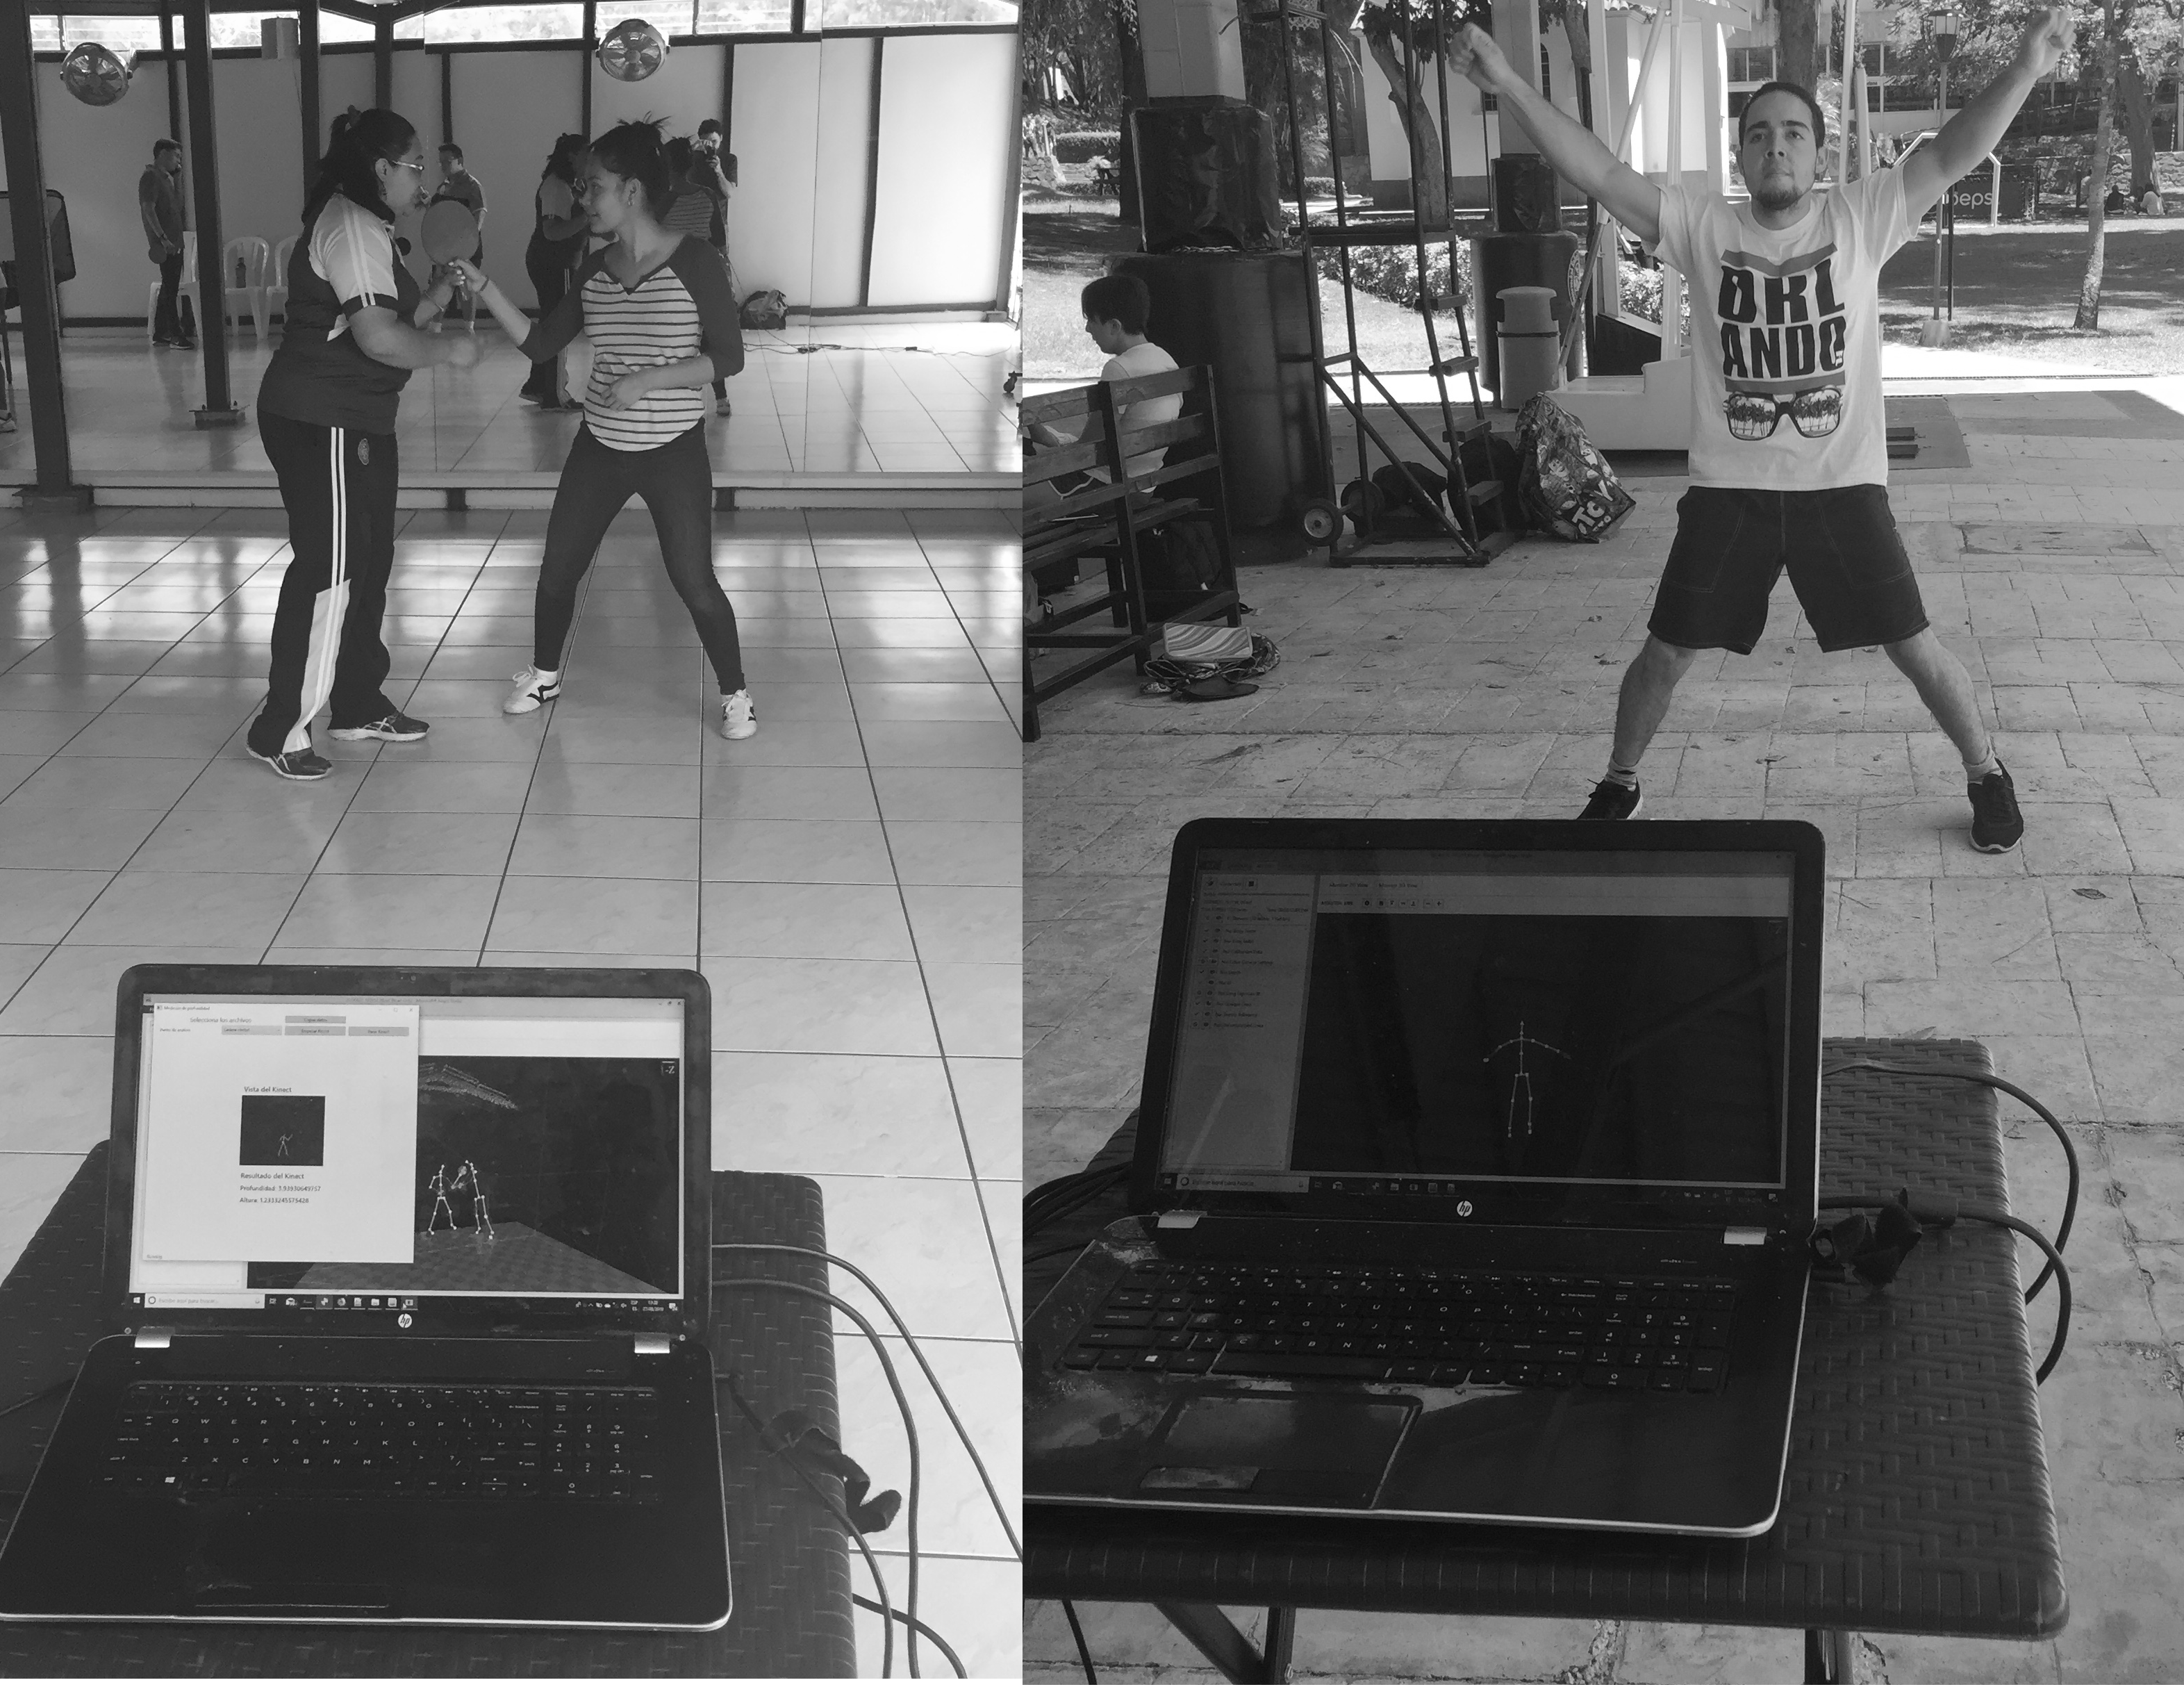
\includegraphics[width=280px,height=280px]{graphics/tomaDatos.png} \\
	\textbf{Fuente:} Propia
\end{figure} 
\subsection{Documentaci\'on del movimiento}
El investigador realiz\'o una breve entrevista a cada entrenador y algunos atletas (similar a un grupo focal), con la finalidad de detallar todos los aspectos de los movimientos, adem\'as de definir los pasos requeridos de cada movimiento v\'alido. Posteriormente a la entrevista, el investigador complet\'o todos los formularios respectivos de movimiento (Formularios de datos de entradas):
\subsubsection{Formularios de entradas de tenis de mesa}
\begin{figure}[H]
	\caption{Formulario de movimiento de tenis de mesa}
	\label{fig:frmMovTen}
	\centering	\includegraphics[width=445px,height=600px]{graphics/resultados/movimientoTenis.PNG} \\
	\textbf{Fuente:} Elaborado por el autor de tesis con base a las observaciones del trabajo de campo
\end{figure}
\begin{figure}[H]
	\caption{Formulario de rutina de tenis de mesa}
	\label{fig:frmRoutTen}
	\centering	\includegraphics[width=445px,height=600px]{graphics/resultados/rutina-tennis.PNG} \\
	\textbf{Fuente:} Propia
\end{figure}
\subsubsection{Formularios de entradas de animaci\'on}
\begin{figure}[H]
	\caption{Formulario de movimiento de animaci\'on}
	\label{fig:frmMovCheer}
	\centering	\includegraphics[width=445px,height=600px]{graphics/resultados/movimientoCheerleader.PNG} \\
	\textbf{Fuente:} Propia
\end{figure}
\begin{figure}[H]
	\caption{Formulario de rutina de animaci\'on}
	\label{fig:frmRoutCher}
	\centering	\includegraphics[width=400px,height=490px]{graphics/resultados/rutina-cheerleaders.PNG} \\
	\textbf{Fuente:} Propia
\end{figure}
\subsubsection{Formularios de entradas de taekwondo}
\begin{figure}[H]
	\caption{Formulario de movimiento taekwondo}
	\label{fig:frmWhiteMov}
	\centering	\includegraphics[width=445px,height=600px]{graphics/resultados/movimientoTaekwondo.PNG} \\
	\textbf{Fuente:} Propia
\end{figure}
\begin{figure}[H]
	\caption{Formulario de rutina de taekwondo}
	\label{fig:frmRoutTaek}
	\centering	\includegraphics[width=445px,height=600px]{graphics/resultados/rutina-taekwondo.PNG} \\
	\textbf{Fuente:} Propia
\end{figure}
\subsection{Etiquetaci\'on de v\'ideos}
El investigador cre\'o desde cero, una base de datos de gesturas por movimiento (a partir del instrumento Visual Gesture Builder), luego se adjunt\'o a la base de datos, todos los v\'ideos recuperados de la actividad de la toma de datos, y por cada v\'ideo se analiz\'o fotograma por fotograma, asignando un valor a cada paso del movimiento, tal como se muestra en la figura de proceso de etiquetaci\'on del movimiento:
 \begin{figure}[H]
	\caption{Proceso de etiquetaci\'on del movimiento derecha}
	\label{fig:getTag}
	\centering
	\includegraphics[width=250px,height=250px]{graphics/etiquetas.png} \\
	\textbf{Fuente:} Propia
\end{figure} 
\subsection{Construcci\'on y pruebas del modelo}
Por cada modelo, el investigador separ\'o los v\'ideos etiquetados en dos partes:
\begin{itemize}
\item \textbf{V\'ideos para el entrenamiento y construcci\'on del modelo:} Elementos que permiten  entrenar el modelo, generando un archivo de base de datos de gesturas (.gdb), la cual proporciona el valor del factor de movimiento a partir del algoritmo Random Forest Regression.
\item \textbf{V\'ideos para an\'alisis:} El investigador seleccion\'o el archivo de bases de datos de gesturas, y posteriormente la herramienta analiz\'o cada v\'ideo, proporcionando el valor real y pronosticado del modelo, tal como se muestra en la figura de obtenci\'on de valores, el valor real es de 0.008018661, mientras que el valor pronosticado es de \num{103893e-6}:
\end{itemize}
 \begin{figure}[H]
	\caption{Obtenci\'on del valor real y pronosticado}
	\label{fig:getError}
	\centering
	\includegraphics[width=300px,height=300px]{graphics/getError.png} \\
	\textbf{Fuente:} Propia
\end{figure} 
\subsection{Selecci\'on y aceptaci\'on del modelo}
\begin{itemize}
\item \textbf{Selecci\'on:} El investigador realiz\'o tres submodelos distintos por movimiento, con distintos datos de entrenamiento (combinaciones de v\'ideos de entrenamientos y an\'alisis). As\'i mismo por cada submodelo se analiz\'o un v\'ideo de an\'alisis, tabulando los datos reales y pronosticado en una hoja de observaciones (Ver anexos, tabla \ref{tab:obsErrores}). Posteriormente al proceso de tabulaci\'on, se calcul\'o los errores correspondientes de cada modelo (error medio pronosticado, desviaci\'on media absoluta y la ra\'iz del error cuadr\'atico medio), seleccionando as\'i el modelo que tenga un menor error. 
\item \textbf{Aceptaci\'on:} El investigador  verifica la media de los errores de cada submodelo, en caso que el error sea mayor o igual  a un medio del valor de reconocimiento (valor recuperado por los formularios del paso de documentaci\'on del movimiento) se rechaza el modelo, en caso contrario, se da la aprobaci\'on y se construye los intervalos de confianza de detecci\'on de los pasos de un movimiento v\'alido, adem\'as de calcular los porcentajes de detecci\'on de movimiento v\'alido e inv\'alido.
\end{itemize}
\subsection{Extracci\'on de datos de los v\'ideos}
Por cada modelo aceptado, el investigador extrajo los datos del tiempo y el recorrido de la mu\~neca derecha de una repetici\'on, con el fin de objetivo de validar que cada modelo fue entrenado con distintos datos, reflejado en una  regresi\'on de tiempo y recorrido. Lo cual para construir dicha regresi\'on, el investigador separ\'o por cada v\'ideo, los renglones de fotogramas de una repetici\'on, listando los tiempos iniciales y finales utilizado para la extracci\'on de datos de v\'ideos .xef (recuperado del instrumento, Kinect studio).
\begin{figure}[H]
	\caption{Segmentos de repeticiones de un v\'ideo}
	\label{fig:segVideo}
	\centering
	\includegraphics[width=420px,height=100px]{graphics/separarPuntos.PNG} \\
	\textbf{Fuente:} Propia
\end{figure} 
\subsection{Validaci\'on  del modelo en tiempo real}
El investigador realiz\'o una \'ultima visita a cada equipo deportivo (cuyo modelo fue aprobado), en dicha visita instal\'o el prototipo del modelo en lugar asignado (en paralelo, los atletas realizaban el calentamiento), posteriormente a la instalaci\'on, el investigador le ense\~n\'o al entrenador una versi\'on de prueba de una rutina tabata, dicha prueba lo realiz\'o el investigador (cabe resaltar que el investigador vest\'ia deportivamente y adem\'as ejecut\'o previamente los ejercicios de calentamiento) con una rutina de 1 serie de 10 segundos de descanso y 50 segundos de trabajo. Luego de la prueba, el entrenador seleccion\'o a un grupo de atletas que no participaron en el proceso de toma de datos, y posteriormente se le program\'o a cada atleta del grupo, una rutina tabata (cada deportista se posicion\'o en la distancia de profundidad recomendada).
 \begin{figure}[H]
	\caption{Fotograf\'ias durante la validaci\'on del modelo}
	\label{fig:getvalidationStep}
	\centering
	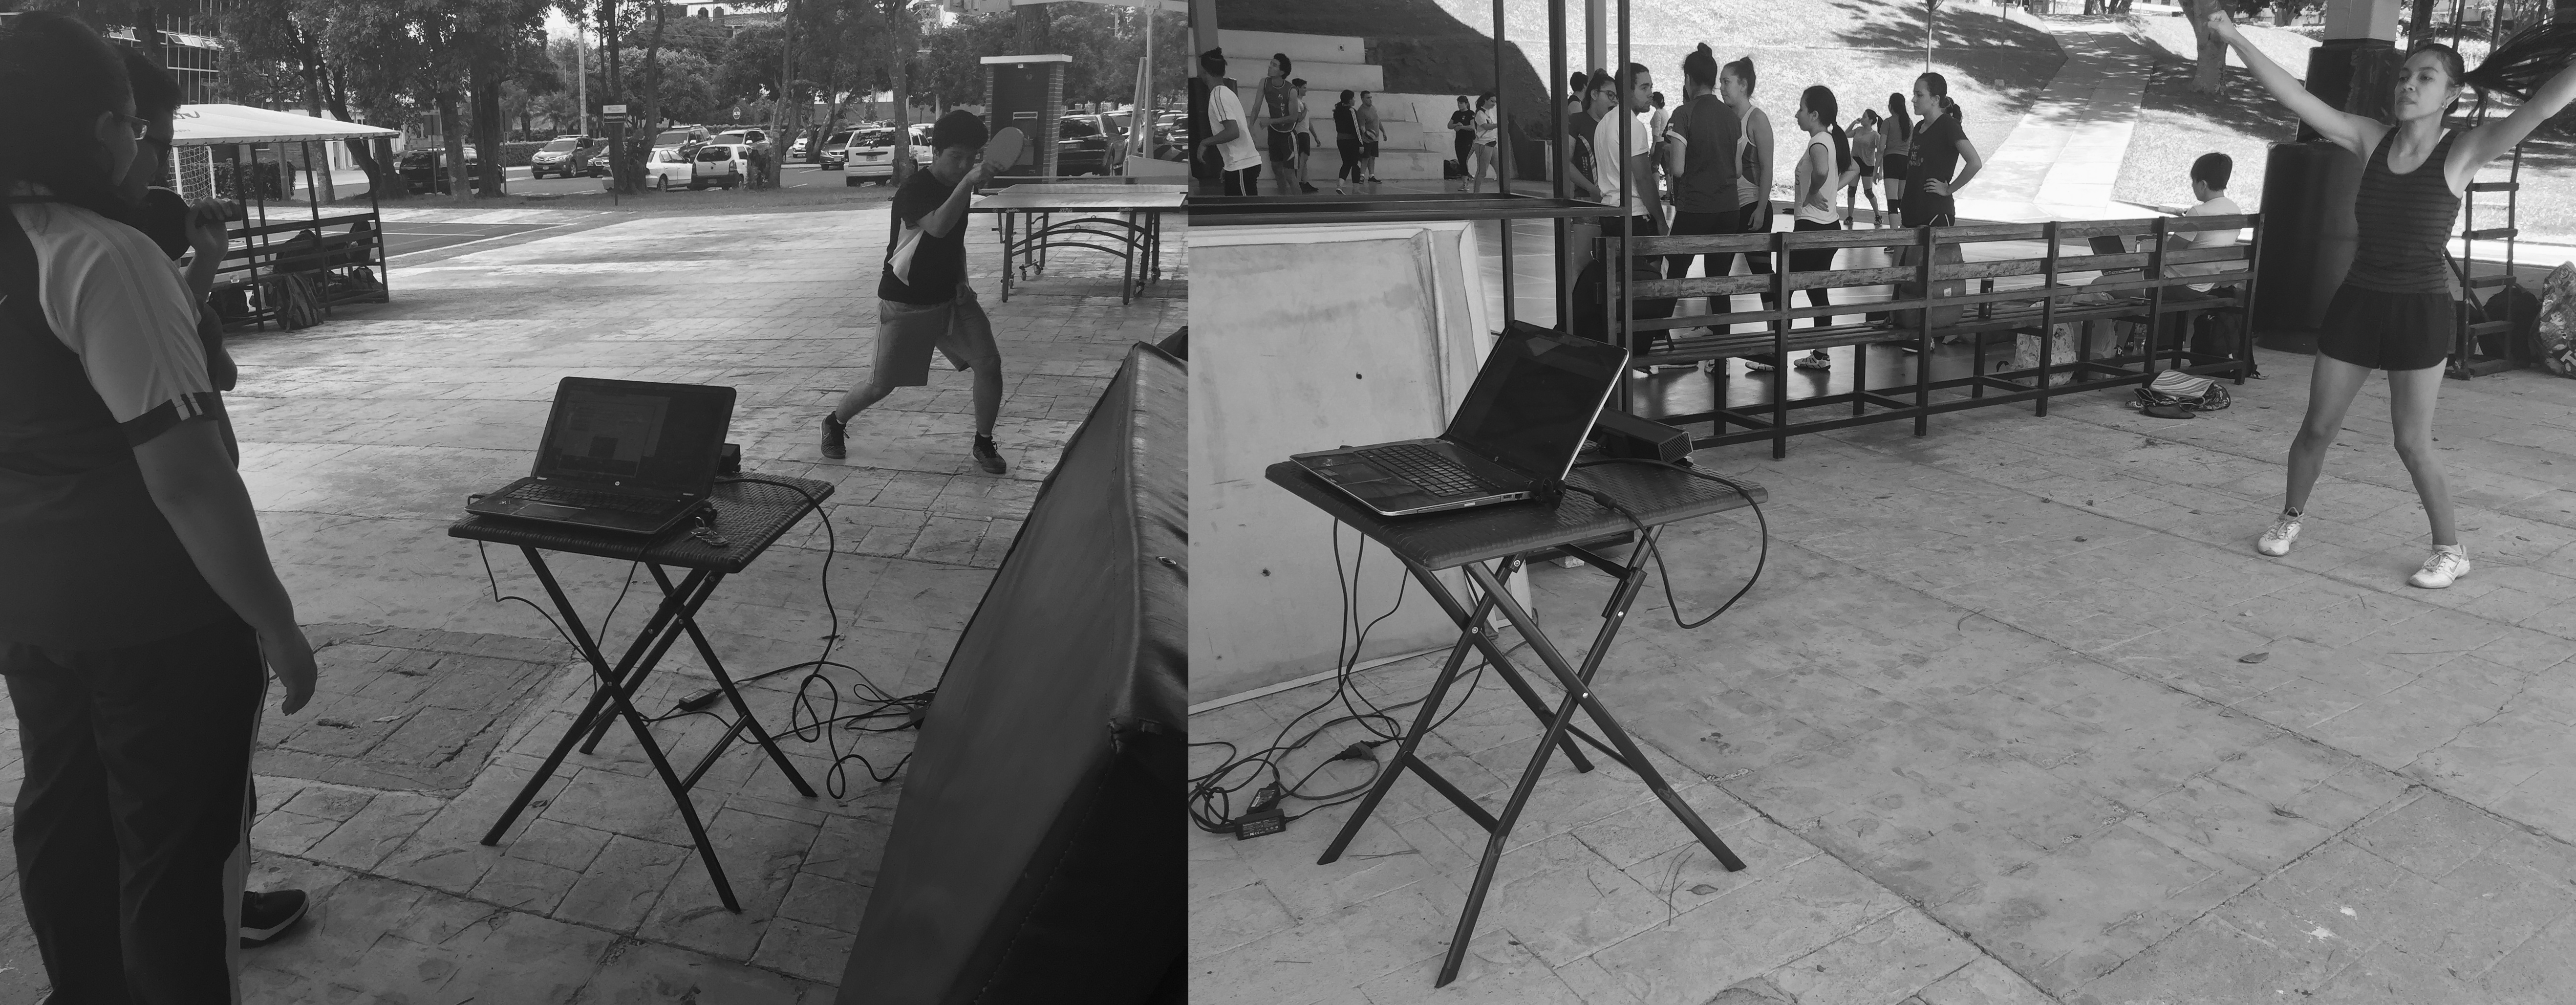
\includegraphics[width=165px,height=165px]{graphics/tabataResultados.png} \\
	\textbf{Fuente:} Propia
\end{figure} 
\section{Dise\~no de la metodolog\'ia}\label{dis}
Esta secci\'on se presenta todos los dise\~nos y c\'alculos matem\'aticos y estad\'isticos encontrados en los resultados. 
\subsection{Asignaci\'on de valores de etiquetas y rangos de identificaci\'on}\label{dis:asig}
Estos valores permiten identificar el paso de cada movimiento a partir de las siguientes variables:
\begin{itemize}
\item \textbf{Offset:} Valor de distribuci\'on de etiquetas de cada paso del movimiento, por partes iguales.
\begin{formula}[H]
	\centering
	\caption{Offset de etiquetas}
	\label{frm:offsetEt}
	\begin{equation}
offset = \frac{1}{pasos-1}
	\end{equation}
	\textbf{Fuente:} Propuesto por el autor de tesis
\end{formula}
\item \textbf{Vector de etiquetas:} A cada paso se le distribuye un valor \'unico, cuyo valor se calcula a partir del offset de la etiqueta anterior.
\begin{formula}[H]
	\centering
	\caption{Asignaci\'on de etiquetas}
	\label{frm:vecEtiq}
	\begin{equation}
\begin{matrix}
etiquetas=[0, etiqueta(1), ..., etiqueta(paso), ..., 1],\; donde
\\
\\
etiqueta(paso) =
\left\{\begin{matrix}
0 & Si\; es\; el\; primer \; paso
\\
etiqueta(paso-1)+offset & Si\; es\; un\; paso\; intermedio
\\ 
1 & Si\; es\; el\; \acute{u}ltimo\; paso
\end{matrix}\right.
\end{matrix}
	\end{equation}
	\textbf{Fuente:} Propuesto por el autor de tesis
\end{formula} 

\item \textbf{Valor de identificaci\'on:} N\'umero que representa la distribuci\'on de reconocimiento  de pasos por partes iguales:
\begin{formula}[H]
	\centering
	\caption{Valor de identificaci\'on de pasos}
	\label{frm:idenStep}
	\begin{equation}
valor \: de \: identificaci\acute{o}n = \frac{1}{pasos}
	\end{equation}
	\textbf{Fuente:} Propuesto por el autor de tesis
\end{formula} 

\item \textbf{Rango de identificaci\'on:} Rango m\'aximo num\'erico para identificar un paso.
\begin{formula}[H]
	\centering
	\caption{Rango m\'aximo de identificaci\'on de un paso}
	\label{frm:idenStep}
	\begin{equation}
\begin{matrix}
rango = [[inferior,superior]] \\
\\
rango(paso)=\left\{\begin{matrix}
inferior(paso)= \left\{\begin{matrix}
0 & paso\: inicial\\ 
superior(paso-1) & paso\: no\: inicial
\end{matrix}\right.\\ 
\\
superior(paso)= \left\{\begin{matrix}
inferior(paso)+identificaci\acute{o}n & paso\, no\, final\\ 
1 & paso\: final

\end{matrix}\right.\\ 
\end{matrix}\right.
\end{matrix}
	\end{equation}
	\textbf{Fuente:} Propuesto por el autor de tesis
\end{formula} 
\end{itemize}
\subsection{C\'alculo indirecto de la altura del usuario} \label{dis:height}
Para el presente proyecto se midi\'o la altura del usuario, a partir de la diferencia entre la altura de la cabeza y la altura promedio de los pies.
	\begin{formula}[H]
	\centering
	\caption{Altura del usuario}
	\label{frm:alturaUser}
	\begin{equation}
y_{usuario}=y_{cabeza}-\frac{y_{pie \: derecho}+y_{pie \: izquierdo}}{2}
	\end{equation}
			\textbf{Fuente:} Planteado por el autor de tesis
\end{formula} 
\subsection{C\'alculo de distancia de profundidad m\'inima y m\'axima} \label{dis:deep}
Para los siguientes c\'alculos se utilizaron la hoja de observaciones de profundidad (Ver anexo, tabla  \ref{tab:obsDepth}), aplicando las siguientes funciones de microsoft excel (versi\'on ingl\'es):
\begin{itemize}
       \item \textbf{Average}: Funci\'on para determinar la altura promedio.
\begin{formula}[H]
	\centering
	\caption{C\'alculo de altura promedio}
	\label{frm:avgHeight}
	\begin{equation}
	Altura \: promedio =AVERAGE([Altura])
	\end{equation}
		\textbf{Fuente:} Elaborado por el autor, a partir de funci\'on de excel
\end{formula}
       \item \textbf{Stdev}: Funci\'on para determinar la desviaci\'on est\'andar de la altura.
\begin{formula}[H]
	\centering
	\caption{C\'alculo de desviaci\'on est\'andar de la altura}
	\label{frm:stdevHeight}
	\begin{equation}
	desviaci\acute{o}n \:  de \: altura =STDEV([Altura])
	\end{equation}
		\textbf{Fuente:} Elaborado por el autor, a partir de funci\'on de excel
\end{formula}
       \item \textbf{Max}: Funci\'on para determinar la profundidad m\'axima entre el Kinect y el atleta.
       \begin{formula}[H]
	\centering
	\caption{C\'alculo de la profundidad m\'axima}
	\label{frm:maxDepth}
	\begin{equation}
	Profundidad \: Max =MAX([Profundidad])
	\end{equation}
		\textbf{Fuente:} Elaborado por el autor, a partir de funci\'on de excel
\end{formula}
       \item \textbf{Min}: Funci\'on para determinar la profundidad m\'inima entre el Kinect y el atleta.
              \begin{formula}[H]
	\centering
	\caption{C\'alculo de la profundidad m\'inima}
	\label{frm:minDepth}
	\begin{equation}
	Profundidad \:  Min =MIN([Profundidad])
	\end{equation}
		\textbf{Fuente:} Elaborado por el autor, a partir de funci\'on de excel.
\end{formula}
\end{itemize}
\subsection{Eventos del Kinect} \label{dis:even}
De acuerdo a la hoja de observaciones de extracci\'on de datos de v\'ideos (Ver tabla \ref{tab:obsVideoData}), se recupera la siguiente informaci\'on:
\begin{itemize}
\item \textbf{Eventos}: Conjunto de datos del seguimiento del esqueleto, durante un intervalo de tiempo.
\begin{formula}[H]
	\centering
	\caption{Matriz de eventos del Kinect}
	\label{frm:event}
	\begin{equation}
\begin{matrix}
Esqueleto & [SkeletonId, Joint, status, x, y, z] \\ 
Evento & [EventoIndex, TotalTime, esqueleto]  \\
\\ 
Eventos & 
\left.\begin{matrix}
Tiempo \: inicial\\ 
\\ 
\\
Tiempo \: final
\end{matrix}\right\}
\begin{matrix}
\left.\begin{matrix}
Evento \: inicial 
\end{matrix}\right\}\\ 
\left.\begin{matrix}
.. \\ 
Eventos \: no \: iniciales \\ 
 ..
\end{matrix}\right\}
\end{matrix}
\begin{bmatrix}
Evento_{0}\\ 
Evento_{1}\\ 
Evento_{2}\\ 
Evento_{x}
\end{bmatrix}
\end{matrix}
	\end{equation}
		\textbf{Fuente:} Propuesto por el autor de tesis.
\end{formula}
\item \textbf{Tiempo relativo}: Describe el tiempo de la repetici\'on, cuyo valor significa la diferencia entre el tiempo total de un evento no inicial y el tiempo total del primer evento.
              \begin{formula}[H]
	\centering
	\caption{C\'alculo del tiempo de la repetici\'on}
	\label{frm:relativeTime}
	\begin{equation}
	relative \: time = TotalTime_{Evento\: x}-TotalTime_{Evento\: inicial}
	\end{equation}
		\textbf{Fuente:} Propuesto por el autor de tesis.
\end{formula}
\item \textbf{Distancia euclidiana}: Describe el desplazamiento de una articulaci\'on, bas\'andose en la posici\'on del primer evento inicial y la posici\'on de un evento no inicial:
\begin{formula}[H]
	\centering
	\caption{Desplazamiento de una articulaci\'on}
	\label{frm:desplazaUser}
	\begin{equation}
|r|=\sqrt{(x_{joint}-x_{o})^{2}+(y_{joint}-y_{o})^{2}+(z_{joint}-z_{o})^{2}}
	\end{equation}
	\textbf{Fuente:} Distancia euclidiana \cite[p.~423]{ayres2001calculo}
\end{formula}  
\end{itemize}
\subsection{Captura de datos durante una rutina (normalizaci\'on de datos)}\label{dis:recognitionMove}
Durante la rutina, los datos del seguimiento del esqueleto son recuperados a partir del kit de desarrollo de software del Kinect, dichos datos son almacenados en la siguiente estructura:
\begin{itemize}
\item \textbf{I:} Valor num\'erico \'unico que identifica una articulaci\'on.
\item \textbf{X:} Posici\'on horizontal de la articulaci\'on, dibujado en una imagen de dos dimensiones.
\item \textbf{Y:} Posici\'on vertical de la articulaci\'on, dibujado en una imagen de dos dimensiones.
\item \textbf{Fm:} Factor del movimiento proporcionado por la base de datos de gesturas.
\item \textbf{P:} Valor num\'erico que identifica el paso que est\'a realizando un atleta.
\item \textbf{Tiempo:} Tiempo de captura de datos.
\item \textbf{Joint:} Vector que almacena la posici\'on de una articulaci\'on en una figura de dos dimensiones.
\item \textbf{Esqueleto:} Vector que almacena todos los vectores de articulaciones del esqueleto humano.
\item \textbf{Step:} Vector que almacena informaci\'on del seguimiento del esqueleto, factor del movimiento y el tiempo de un paso.
\item \textbf{Repetici\'on:} Vector que almacena la informaci\'on de cada de paso de un movimiento.
\item \textbf{Serie:} Vector que almacena las repeticiones del movimiento durante una serie.
\item \textbf{Series:} Vector que almacena la informaci\'on de cada serie de la rutina.
\end{itemize}
\begin{formula}[H]
	\centering
	\caption{Matriz de datos capturados durante una rutina}
	\label{frm:MatrizDatosRepeticion}
	\begin{equation}
\begin{matrix}
i & enumerador\: de\: la\: articulaci\acute{o}n \\ 
x & distancia\, horizontal \: (p\acute{i}xeles) \\ 
y & distancia\, vertical\: (p\acute{i}xeles) \\ 
joint_{i}& [i,x,y] \\ 
 & \\ 
esqueleto & \begin{bmatrix}
joint_{0} \\ 
... \\ 
joint_{i}\\ 
... \\ 
joint_{24}
\end{bmatrix}  \\ 
 & \\ 
fm & factor \, del \, movimiento \\ 
p  & paso \, del \,movimiento \\ 
t  & tiempo \, total \\ 
step_{p}  & [fm,p,esqueleto, tiempo] \\
 & \\ 
Repeticion & [step_{0}, ...,  step_{col}, ..., step_{last}] \\
serie & [repeticion] \\
series & [serie]
\end{matrix}
	\end{equation}
	\textbf{Fuente:} Propuesto por el autor de tesis
\end{formula}
\subsection{Validaci\'on del modelo de reconocimiento de movimiento}\label{dis:validate}
El presente proyecto se utiliz\'o dos m\'etodos de validaciones cruzadas \cite{perez2015analisis}:
\begin{itemize}
\item \textbf{Hold out:} Las muestras de datos se separan en dos conjunto, uno para construir y entrenar el modelo -i.e. Build- y otro para realizar pruebas que dan validez a los m\'argenes  de errores del modelo.
\item \textbf{K-fold:} Las muestras se dividen en K subconjuntos, y en cada subconjunto se aplica el m\'etodo hold out.
\end{itemize}  
\begin{table}[H]
\begin{center}
\caption{Validaci\'on cruzada, 3-fold de tenis de mesa}
\label{tab:KfoldTenis}
\begin{tabular}{|l|l|l|}
\hline
\multicolumn{3}{|c|}{\textbf{Muestra de v\'ideos}} \\ \hline
\multicolumn{3}{|c|}{1, 2, 3, 4, 5, 6} \\ \hline
\textbf{Modelo} & \textbf{Builds} & \textbf{Test} \\ \hline
1 & 1, 2, 3, 4, 5 & 6 \\ \hline
2 & 1, 2, 4, 5, 6 & 3 \\ \hline
3 & 2, 3, 4, 5, 6 & 1 \\ \hline
\multicolumn{3}{l}{\textbf{Fuente:} Propia}
\end{tabular}
\end{center}
\end{table}
\begin{table}[H]
\begin{center}
\caption{Validaci\'on cruzada, 3-fold de animaci\'on}
\label{tab:KfoldAnimacion}
\begin{tabular}{|l|l|l|}
\hline
\multicolumn{3}{|c|}{\textbf{Muestra de v\'ideos}} \\ \hline
\multicolumn{3}{|c|}{1, 2, 3, 4, 5, 6, 7} \\ \hline
\textbf{Modelo} & \textbf{Builds} & \textbf{Test} \\ \hline
1 & 1, 2, 3, 4, 5, 6 & 1 \\ \hline
2 & 1, 2, 3, 5, 6, 7 & 4 \\ \hline
3 & 1, 2, 3, 4, 5, 6 & 7 \\ \hline
\multicolumn{3}{l}{\textbf{Fuente:} Propia}
\end{tabular}
\end{center}
\end{table}
\begin{table}[H]
\begin{center}
\caption{Validaci\'on cruzada, 3-fold de taekwondo}
\label{tab:KfoldTaekwondo}
\begin{tabular}{|l|l|l|}
\hline
\multicolumn{3}{|c|}{\textbf{Muestra de videos}} \\ \hline
\multicolumn{3}{|c|}{1, 2, 3, 4, 5, 6, 7, 8, 9, 10, 11, 12, 13, 14, 15, 16} \\ \hline
\textbf{Modelo} & \textbf{Builds} & \textbf{Test} \\ \hline
1 & 1, 2, 3, 4, 5, 6, 7, 8, 9, 11, 12, 13, 14, 15, 16 & 10 \\ \hline
2 & 1, 2, 3, 4, 5, 6, 7, 8, 9, 10, 12, 13, 14, 15, 16 & 11 \\ \hline
3 & 1, 2, 3, 4, 5, 6, 7, 8, 9, 10, 11, 13, 14, 15, 16 & 12 \\ \hline
\multicolumn{3}{l}{\textbf{Fuente:} Propia}
\end{tabular}
\end{center}
\end{table}
Posteriormente en la etapa de pruebas, se realiz\'o  por cada modelo una hoja de observaciones de valores reales y pronosticados (ver anexo, tabla \ref{tab:obsErrores}), de modo de encontrar los siguientes errores de pron\'osticos \cite{erroresPronostico}:
\begin{itemize}
\item \textbf{Error medio pronosticado (\acrshort{EMP}):} Promedio de diferencia entre el valor real y pronosticado, la cual puede tener tres interpretaciones distintas:
	\begin{itemize}
	\item \textbf{Valor positivo:} En promedio, los valores pronosticado est\'an por debajo de los valores reales.
	\item \textbf{Valor negativo:} En promedio, los valores pronosticado est\'an por arriba de los valores reales.
	\item \textbf{Valor cero:} Los valores pronosticados pueden estar por debajo o por arriba de los valores reales.
	\end{itemize}
\begin{formula}[H]
	\centering
	\caption{C\'alculo del error medio pronosticado}
	\label{frm:empMath}
	\begin{equation}
EMP=\frac{\sum_{0}^{n}(Real_{x}-Pronostic_{x}\cdot10^{-6})}{n}
	\end{equation}
	\textbf{Fuente:} Formula adaptada al proyecto, a partir de la f\'ormula del error medio pronosticado \cite{videoErrores}
\end{formula}  
\item \textbf{Desviaci\'on media absoluta (\acrshort{DMA}):} Promedio de diferencia absoluta entre el valor real y pronosticado, que muestra la dispersi\'on con respecto al valor real.
 \begin{formula}[H]
	\centering
	\caption{C\'alculo de la desviaci\'on media absoluta}
	\label{frm:MADMath}
	\begin{equation}
DMA=\frac{\sum_{0}^{n}( \left |  Real_{x}-Pronostic_{x}\cdot10^{-6} \right |)}{n}
	\end{equation}
	\textbf{Fuente:} Formula adaptada al proyecto, a partir de la f\'ormula de la desviaci\'on media absoluta \cite{videoErrores}
\end{formula}  
\item \textbf{Ra\'iz del error cuadr\'atico medio (RECM):} Es la desviaci\'on est\'andar de los errores de predicci\'on, la cual indica qu\'e tan disperso se encuentra los errores con respecto al error medio pronosticado.
 \begin{formula}[H]
	\centering
	\caption{C\'alculo de la ra\'iz del error cuadr\'atico medio}
	\label{frm:RECMMath}
	\begin{equation}
RECM=\sqrt{\frac{\sum_{0}^{n}((Real-Pronostic\cdot10^{-6})-EMP)^{2}}{n}}
	\end{equation}
	\textbf{Fuente:} Formula adaptada al proyecto, a partir de la f\'ormula de la ra\'iz del error cuadr\'atico medio \cite{GEORCMETUT}
\end{formula}  
\end{itemize}
Luego de encontrar los errores, se debe seleccionar el modelo que tenga la menor \acrshort{RECM}, y posteriormente encontrar los errores de la muestra total:
 \begin{formula}[H]
	\centering
	\caption{EMP de la muestra total}
	\label{frm:EmpAll}
	\begin{equation}
EMP_{muestra\, total}=AVERAGE([EMP_{modelo}])
	\end{equation}
	\textbf{Fuente:} Propuesto por el autor de tesis, con base a las f\'ormulas de excel (versi\'on en ingl\'es)
\end{formula}  
 \begin{formula}[H]
	\centering
	\caption{MAD de la muestra total}
	\label{frm:MadAll}
	\begin{equation}
MAD_{muestra\, total}=AVERAGE([MAD_{modelo}])
	\end{equation}
	\textbf{Fuente:} Propuesto por el autor de tesis, con base a las f\'ormulas de excel (versi\'on en ingl\'es)
\end{formula}  
	 \begin{formula}[H]
	\centering
	\caption{RECM de la muestra total}
	\label{frm:RecmAll}
	\begin{equation}
RECM_{muestra\, total}=AVERAGE([RECM_{modelo}])
	\end{equation}
	\textbf{Fuente:} Propuesto por el autor de tesis, con base a las f\'ormulas de excel (versi\'on en ingl\'es)
\end{formula} 
Los errores de la muestra total ayudan aceptar o rechazar el modelo; si la \acrshort{RECM} promedio  es menor a un medio del valor de identificaci\'on se aprueba (se divide entre dos, debido que las etiquetas de los pasos intermedio se encuentra a la mitad de cada rango de identificaci\'on respectiva). En caso que sea mayor o igual, se rechaza, debido que los intervalos de confianza colisiona con otros intervalos de confianza (Intervalos que se utiliza para la detecci\'on de un paso):
\begin{figure}[H]
	\caption{Criterios de aceptaci\'on de un modelo de detecci\'on de los pasos requeridos de un movimiento}
	\label{fig:AproveOrDennie}
	\centering
	\includegraphics[width=430px,height=360px]{graphics/CriterioAceptacion.png} \\
	\textbf{Fuente:} Propia
\end{figure}
En la figura \ref{fig:AproveOrDennie}, se separa en tres partes:
\begin{itemize}
\item \textbf{Detalles generales del movimiento:} Muestra las variables num\'ericas de un movimiento.
\item \textbf{Caso aprobado:} Al construir los intervalos de confianza, se observa que no colisiona entre s\'i.
\item \textbf{Caso rechazado:} Al construir los intervalos de confianza, se observa que los intervalos del paso 1 colisiona con el paso 2 (debido que el intervalo de confianza inferior del paso 2 se encuentra dentro del intervalo de confianza del paso 1), y los intervalos del paso 2 colisiona con el paso 3 (debido que el intervalo de confianza inferior del paso 3 se encuentra dentro del intervalo de confianza del paso 2).
\end{itemize}
Adem\'as, por cada modelo aprobado se debe encontrar los intervalos de confianza  que permite detectar los pasos de un movimiento v\'alido:
\begin{formula}[H]
	\centering
	\caption{Intervalos de confianza de reconocimiento de un paso}
	\label{frm:rangoConfiabilidad}
	\begin{equation}
\begin{matrix}

intervalo\: de\: confianza = ic =[[inferior,superior]] \\
\\
ic(paso)=\left\{\begin{matrix}
inferior(paso)=\left\{\begin{matrix}
0 & si\, es\, el\, primer\, paso\\ \\ 
etiqueta(paso)- RECM_{muestra\, total} & si\: es\: paso\: intermedio \\ 
\\
1-RECM_{muestra\, total}& si\, es\, el\, \acute{u}ltimo\, paso
\end{matrix}\right. \\ 
\\ 
inferior(paso)=\left\{\begin{matrix}
RECM_{muestra\, total}& si\, es\, el\, primer\, paso \\
\\
etiqueta(paso)+RECM_{muestra\, total} & si\: es\: paso\: intermedio \\ \\ 
1 & si\: es\: el\: \acute{u}ltimo\: paso
\end{matrix}\right.
\end{matrix}\right.
\end{matrix}
	\end{equation}
	\textbf{Fuente:} Propuesto por el autor de tesis
\end{formula} 
Por otro lado, se debe determinar el valor de recognition, n\'umero porcentual que determina el porcentaje de detecci\'on similar al fotograma de cada paso respectivo, es decir:
 \begin{itemize}
\item \textbf{Porcentaje mayor a cero:} Entre m\'as cercano al 100\%, el factor de movimiento es similar al valor de etiquetado (menor error).
\item \textbf{Porcentaje menor o igual a cero:} Son modelos rechazado, debido que el error es grande y adem\'as no detecta los pasos de un movimiento (por colisiones de los intervalos de confianza).
\end{itemize}
\begin{formula}[H]
	\centering
	\caption{Valor de recognition}
	\label{frm:Recognitiona}
	\begin{equation}
recognition=1-no\,v\acute{a}lidos=1-\frac{RECM_{muestra\, total}}{valor\: de\: identificaci\acute{o}n}  
	\end{equation}
	\textbf{Fuente:} Propuesto por el autor de tesis
\end{formula}
\subsection{Algoritmo clasificador de un movimiento v\'alido}\label{dis:algoritmoDet}
Se presenta el algoritmo clasificador de repetici\'on de un movimiento v\'alido:
\begin{itemize}
\item Entradas:
\begin{itemize}
\item \textbf{Paso siguiente:} Variable que lleva el control del orden de todos los pasos detectados.
\item \textbf{Factor del movimiento:} Variable que indica la transici\'on del movimiento a partir del algoritmo Random Forest Regression.
\item \textbf{Paso detectado:} Variable que indica el paso actual del factor del movimiento.
\item \textbf{Paso no detectado:} Variable que no tiene un valor al inicio, la cual se asigna un valor en el caso que sea una repetici\'on inv\'alida (indica el paso del fallo del movimiento).
\end{itemize}
\item Procesos:
\begin{enumerate}[1.]
\item Asignar el paso siguiente como paso inicial (paso No.1), debido que marca el inicio de la repetici\'on. %1
\item Capturar un nuevo fotograma del Kinect, y obtiene el factor del movimiento del respectivo fotograma, a partir del algoritmo Random Forest Regression y la herramienta, Visual Gesture Builder. %2
\item Verificar si el factor del movimiento se encuentra en alg\'un intervalo de confianza para obtener el paso detectado, en caso que no se encuentre, no devolver\'a ning\'un valor.  %3
\item Verificar si el paso detectado tiene un valor, adem\'as de chequear que no sea un valor anterior (valor anterior del paso siguiente), en caso que no cumpla ambas condiciones, se debe esperar a capturar un nuevo fotograma (Volver al proceso No.2). %4
\item Verificar si el paso detectado es igual al paso siguiente, en caso que sea diferente se detect\'o una repetici\'on inv\'alida (saltar al proceso No. 9). %5
\item Verificar si el paso detectado es el \'ultimo paso, en caso contrario (saltar al proceso No. 8) %6
\item Finalizar algoritmo con repetici\'on v\'alida. %7 
\item Incrementar el paso siguiente y volver a obtener un nuevo fotograma del Kinect (saltar al proceso No. 2). %8
\item Asignar el paso no detectado como paso siguiente.
\item Finalizar el algoritmo con repetici\'on inv\'alida.
\end{enumerate}
\item Salidas:
\begin{itemize}
\item \textbf{Repetici\'on v\'alida:} El usuario pas\'o por todos los pasos de un movimiento v\'alido de forma ordenada.
\item \textbf{Repetici\'on inv\'alida y su paso no detectado:} El usuario se salt\'o el paso no detectado, lo cual genera un movimiento inv\'alido.
\end{itemize}
\end{itemize}
\begin{figure}[H]
	\caption{Algoritmo clasificador de repetici\'on de un movimiento v\'alido }
	\label{fig:capturaDatos}
	\centering
	\includegraphics[width=430px,height=630px]{graphics/flujoGramaRepiticion.png} \\
	\textbf{Fuente:} Propia.
\end{figure}
Este algoritmo es aplicado para analizar los v\'ideos de testeos, debido que se etiquetaron  repeticiones de movimientos v\'alidos.  Sin embargo, al comparar los factores del movimiento de los fotogramas (de los v\'ideos de testeos), pueden ocurrir que no reconozca un paso, por lo tanto la repetici\'on del movimiento v\'alido se convierte en inv\'alido:
 \begin{figure}[H]
	\caption{Clasificaci\'on de repeticiones de movimiento v\'alido o inv\'alido  en un v\'ideo de testeo}
	\label{fig:detValido}
	\centering
	\includegraphics[width=430px,height=450px]{graphics/reconocimientoDePasos.png} \\
	\textbf{Fuente:} Propia.
\end{figure}
En la figura \ref{fig:detValido}, se divide en tres partes:
\begin{itemize}
\item \textbf{Intervalos de confianza:} Tabla que permite reconocer los pasos del movimiento, si el factor del movimiento se encuentra dentro del intervalo de confianza.
\item \textbf{Repetici\'on v\'alida:} Es v\'alido,  ya que detecta todos los pasos de manera ordenada  durante los fotogramas: Uno, tres y seis (observe que los factores del movimiento se encuentran dentro del alg\'un intervalo de confianza). 
\item \textbf{Repetici\'on inv\'alida:} Es inv\'alido, debido que para el fotograma 6, se esperaba detectar el paso dos (paso siguiente), pero se detect\'o el paso tres, por lo tanto el algoritmo determina que es una repetici\'on inv\'alida.
\end{itemize}
Este procedimiento permite completar la tabla de observaciones de clasificaci\'on de cada v\'ideo de testeo (ver anexos, tabla \ref{tab:DetectarPasoCorrecto}), en donde por cada repetici\'on etiquetada se verifica todos los pasos, por medio de tres valores:
\begin{itemize}
\item \textbf{Verdadero:} Si se detect\'o el paso correspondiente (de manera ordenada).
\item \textbf{Falso:} Repetici\'on invalida debido que no se detect\'o el paso correspondiente. 
\item \textbf{Sin valor:} El algoritmo no determin\'o ning\'un valor, debido que finaliz\'o al momento  que detect\'o una repetici\'on inv\'alida.
\end{itemize}
Por otra parte, se puede determinar el porcentaje de v\'alido e inv\'alidos del modelo de clasificador de repeticiones, adem\'as de determinar el porcentaje de cada paso no detectado:
\begin{formula}[H]
	\centering
	\caption{Porcentajes del modelo de clasificador}
	\label{frm:porcentajeClasificador}
	\begin{equation}
\begin{matrix}
repeticiones\: v\acute{a}lidas = contarSi(\acute{u}ltimo\: paso\: es\: verdadero) \\ 
 \\ 
repeticiones\: inv\acute{a}lidas = repeticiones\; totales\: del\: video - repeticiones\: v\acute{a}lidas\\ 
 \\ 
\%_{v\acute{a}lidos}=\frac{repeticiones\: v\acute{a}lidas}{repeticiones\; totales\: del\: video}\\ 
\\
\%_{inv\acute{a}lidos}=\frac{repeticiones\: inv\acute{a}lidas}{repeticiones\; totales\: del\: video}\\ 
\\ 
\%_{paso\; no\; detectado}=\frac{contarSi(paso\: es\: falso)}{repeticiones\: inv\acute{a}lidas}\\ 
\end{matrix}
	\end{equation}
	\textbf{Fuente:} Propuesto por el autor de tesis
\end{formula}
Es importante saber si el modelo de clasificaci\'on  de un movimiento v\'alido se aprueba, por lo tanto se debe calcular los porcentajes de referencias v\'alido e inv\'alido, que se determinan a partir del peor de los casos (detecta una repetici\'on v\'alida y las posibles combinaciones de una  repetici\'on inv\'alida): 
 \begin{figure}[H]
	\caption{Porcentajes de referencias v\'alidos e inv\'alidos }
	\label{fig:porcValido}
	\centering
	\includegraphics[width=430px,height=300px]{graphics/porceRef.png} \\
	\textbf{Fuente:} Propia.
\end{figure}
A partir de los porcentajes de referencias de clasificaci\'on, se pueden presentar dos casos:
\begin{itemize}
\item \textbf{Clasificaci\'on Aceptable:} Si el porcentaje de detecci\'on v\'alida es mayor al porcentaje de referencia v\'alida (Por consiguiente el porcentaje de detecci\'on inv\'alida es menor al porcentaje de referencia inv\'alida).
\item \textbf{Clasificaci\'on no aceptable:} Si el porcentaje de detecci\'on v\'alida es menor o igual al porcentaje de referencia v\'alida (Por consiguiente el porcentaje de detecci\'on inv\'alida es mayor o igual al porcentaje de referencia inv\'alida). 
\end{itemize}
\subsection{Dise\~no de los resultados de una rutina tabata} \label{dis:results}
En esta secci\'on se determina los resultados de la rutina de tabata, dichos resultados son encontrados a partir del seguimiento del esqueleto, la cual proporciona informaci\'on de las variables de los detalles del paso y repetici\'on (Ver f\'ormula \ref{frm:MatrizDatosRepeticion}), con el fin objetivo de encontrar la siguiente informaci\'on:
\begin{itemize}
\item \textbf{Volumen de repeticiones:} Sumatoria de las cantidades totales de repeticiones de una serie.  
\begin{code}[H]
	\caption{Pseudoc\'odigo para obtener las repeticiones totales de una rutina}
	\label{code:getRepetitions}
	\begin{lstlisting}
Entradas:
	Series de repeticiones del movimiento
	Contador de Repeticiones

Procesos:
	Recorrer cada serie de repeticiones del movimiento:
		Contar las repeticiones de la serie
		Sumar al contador de repeticiones

Salida:
	Contador de repeticiones
	\end{lstlisting}
	\textbf{Fuente:} Propia.
\end{code}

\item \textbf{Duraci\'on:} Tiempo total que se emplea en una rutina, tomando en cuenta todas las series de trabajos y descansos.
\begin{formula}[H]
	\centering
	\caption{C\'alculo de la duraci\'on de tiempo de una rutina}
	\label{eq:DurationTime}
	\begin{equation}
	Duration = \sum_{i=0}^{series}restTime +\sum_{i=0}^{series}workTime = series(restTime+workTime)
	\end{equation}
		\textbf{Fuente:} Elaborado por el autor de tesis
\end{formula}
\item \textbf{Resistencia:} Construye la estructura de la gr\'afica de la resistencia de un atleta durante una rutina a partir del recorrido de todas la series, posteriormente en cada serie se recorre todas las repeticiones y luego en cada repetici\'on se almacena el tiempo acumulado de la rutina y la cantidad de repeticiones que lleva el atleta a ese momento.
\begin{code}[H]
	\caption{Pseudoc\'odigo para crear la gr\'afica de resistencia}
	\label{code:getEndurance}
	\begin{lstlisting}
Entradas:
	Series de repeticiones del movimiento
	Gráfico en donde almacena
		Subgráfico que está compuesto por
			Nombre de la serie
			Listado de puntos en donde cada punto
				Guarda el tiempo (eje x)
				Guarda el numero de repetición (eje y)
	
Proceso:
	Crear gráfico
	Recorrer cada serie de repeticiones del movimiento
		Crear subgráfico
		Obtener el número de serie
		Crear el listado de puntos
		Recorrer cada repetición de la serie
			Obtener el número de repeticiones acumuladas 
			Obtener el tiempo del paso final de la repetición
			Crear un punto
			Guardar punto en el listado de puntos
		Almacenar en el subgráfico el número de serie y listado de puntos
		Guardar subgráfico en el listado que tiene el gráfico

Salida:
	Gráfico de resistencia
	\end{lstlisting}
	\textbf{Fuente:} Propia.
\end{code} 

\item \textbf{Potencia:} Resultado que muestra la cantidad m\'axima de repeticiones en el menor tiempo posible, la cual se encuentra a partir del recorrido de las series, luego en cada serie se determina la cantidad de repeticiones totales y el tiempo acumulado de la \'ultima repetici\'on, encontrando: 
	\begin{itemize}
	\item Una mayor cantidad de repeticiones almacenada anteriormente
	\item La misma cantidad de repeticiones almacenada anteriormente, pero se verifica si el tiempo acumulado es menor.
	\end{itemize}
\begin{code}[H]
	\caption{Pseudoc\'odigo para obtener la potencia}
	\label{code:getEndurance}
	\begin{lstlisting}
Entradas:
	Series de repeticiones del movimiento
	Potencia en donde almacena
		Cantidad de repeticiones acumuladas de una serie
		Tiempo total de la última repetición de la serie
		
Procesos:
	Crear potencia
	Recorrer cada serie de repeticiones del movimiento
		Obtener la última repetición de la serie
			Obtener el número de repeticiones acumuladas
			Obtener el tiempo del paso final de la repetición
			¿El número de repeticiones acumuladas aumentó?
				Si
					Almacenar los datos en potencia
				Sino si, ¿El número de repeticiones permaneció igual?:
					¿El Tiempo total disminuyó?:
						Si
							Almacenar los datos en potencia
						
Salida:
	Potencia 
	\end{lstlisting}
	\textbf{Fuente:} Propia.
\end{code} 

\item \textbf{Velocidad}: Raz\'on de cambio separado por:
	\begin{itemize}
	\item \textbf{Repeticiones por serie:} Variable que se determina a partir del promedio total de repeticiones por serie.
		\item \textbf{Tiempo por repetici\'on:} Variable que se determina a partir del promedio de la diferencia entre el tiempo del paso final y tiempo del paso inicial -i.e. Tiempo de una repetici\'on- de cada repetici\'on realizada por el atleta.
	\end{itemize}
\end{itemize}


\begin{code}[H]
	\caption{Pseudoc\'odigo para obtener las velocidades de las rutinas}
	\label{code:getTimeOfRepetitions}
	\begin{lstlisting}
Entradas:
	Series de repeticiones del movimiento
	Velocidad en donde almacena
		Repeticiones por serie
		Tiempo por serie
		
Proceso:
	Crear velocidad
	Crear un listado de tiempos de repeticiones
	Crear un listado de repeticiones de series
	Recorrer cada serie de repeticiones del movimiento
		Obtener el total de repeticiones de la serie
		Agregar al listado de repeticiones de series
		Recorrer cada repetición de la serie
			Obtener el tiempo del paso inicial de la repetición
			Obtener el tiempo del paso final de la repetición
			Encontrar la diferencia de tiempos del paso final e inicial
			Almacenar en el listado de tiempos de repeticiones
	Encontrar el promedio de repeticiones de series
	Transformar a número entero el promedio de repeticiones de series
	Encontrar el promedio de tiempos de repeticiones
	Almacenar ambos promedios en velocidad
	
Salida:
	Velocidad
	\end{lstlisting}
	\textbf{Fuente:} Propia.
\end{code} 
\section{Criterios del proyecto}\label{criter}
En esta secci\'on se presenta todos los criterios que se siguieron para crear el modelo de reconocimientos de movimientos:
\subsection{Criterios de selecci\'on de movimiento}
\begin{itemize}
	\item El investigador y el entrenador de cada deporte  seleccionaron aquellos movimientos que se ejecutan dentro del \'area de visi\'on del sensor Kinect.
	\item El movimiento no debe ser complejo, es decir que cualquier persona pueda realizar dicho movimiento, sin importar su nivel deportivo.
	\item Debe ser un movimiento que se emplea constantemente en el deporte, para aprender nuevos movimientos complejos.
\end{itemize}
\subsection{Criterios de an\'alisis de movimiento}
\begin{itemize}
	\item Cada movimiento debe tener una articulaci\'on de an\'alisis.
	\item El conjunto de articulaciones que interact\'uan en el movimiento, se debe seleccionar con base a la separaci\'on del cuerpo humano, es decir, la parte inferior (Articulaciones abajo de la cadera central) o superior (Articulaciones arriba de la cadera central).
\end{itemize}
\subsection{Criterios de etiquetaci\'on de movimiento}
\begin{itemize}
	\item Cada repetici\'on del movimiento debe pasar por todos los pasos.
	\item El rango de etiquetaci\'on debe estar entre valores de 0 (paso inicial) y 1 (paso final).
	\item La curva de aprendizaje de cada repetici\'on, debe ser similar a la funci\'on sigmoide -i.e. gr\'afica con forma de ese (s)-.
	\item No se etiqueta los datos de ruidos durante una repetici\'on del movimiento -e.g. Interrupciones, errores en el seguimiento del esqueleto-.
\end{itemize}
\subsection{Criterios de error del modelo}
\begin{itemize}
	\item Se debe calcular la dispersi\'on entre los datos de la muestra y su media, a partir de la ra\'iz del error cuadr\'atico medio (RECM).
	\item Se debe calcular la dispersi\'on entre los datos reales y pronosticado a partir de la desviaci\'on media absoluta (DMA). 
	\item El error se encuentra en un rango de 0 a 1.
\end{itemize}
\subsection{Criterios de selecci\'on del modelo}
\begin{itemize}
	\item Se selecciona el submodelo que contenga la  menor RECM, en caso que exista RECM iguales, se escoge el modelo que tenga la menor DMA.
\end{itemize}
\subsection{Criterios de aceptaci\'on del modelo}
\begin{itemize}
	\item El modelo seleccionado debe considerar los errores de todas las muestras, a partir del promedio de errores de los submodelos comparados.
	\item Se aprueba el modelo, s\'i el valor promedio de la RECM es menor a un medio del valor de  identificaci\'on.
\end{itemize}
\afterpage{\blankpage}
\newpage
\afterpage{\blankpage}
\newpage
\chapter{Presentaci\'on y an\'alisis de resultados}
\section{Distancias de profundidades recomendadas entre el atleta y el sensor} \label{res:idMov}
En la siguiente tabla se muestra un resumen general de las caracter\'isticas de la muestra de cada equipo deportivo, en ella se describe la altura promedio y las distancias recomendadas para ejecutar correctamente el seguimiento del esqueleto (renderizaci\'on completa del esqueleto humano), dichos datos fueron capturados por el sensor Kinect a una altura de 0.70 metros desde el suelo y tomando como punto de referencia, la cadera central de cada atleta:
\begin{table}[H]
\begin{center}
\caption{Distancias de profundidades recomendadas para el funcionamiento del seguimiento del  esqueleto}
\label{tab:depthCalculation}
\begin{tabular}{lllll}
\hline
\multicolumn{3}{|c|}{Caracter\'isticas generales} & \multicolumn{2}{l|}{\begin{tabular}[c]{@{}l@{}}Distancias de profundidades recomendadas \\ entre el usuario y el sensor\end{tabular}} \\ \hline
\multicolumn{1}{|l|}{Deporte} & \multicolumn{1}{l|}{\begin{tabular}[c]{@{}l@{}}Altura promedio\\ (metros)\end{tabular}} & \multicolumn{1}{l|}{\begin{tabular}[c]{@{}l@{}}Desviaci\'on est\'andar\\ de la altura (metros)\end{tabular}} & \multicolumn{1}{l|}{\begin{tabular}[c]{@{}l@{}}M\'inima\\ (metros)\end{tabular}} & \multicolumn{1}{l|}{\begin{tabular}[c]{@{}l@{}}M\'axima\\ (metros)\end{tabular}} \\ \hline
\multicolumn{1}{|l|}{Tenis de mesa} & \multicolumn{1}{l|}{1.302435} & \multicolumn{1}{l|}{+/- 0.088683} & \multicolumn{1}{l|}{3.505103} & \multicolumn{1}{l|}{3.990376} \\ \hline
\multicolumn{1}{|l|}{Animaci\'on} & \multicolumn{1}{l|}{1.342471} & \multicolumn{1}{l|}{+/-0.059301} & \multicolumn{1}{l|}{2.763813} & \multicolumn{1}{l|}{3.411942} \\ \hline
\multicolumn{1}{|l|}{Taekwondo} & \multicolumn{1}{l|}{1.373372} & \multicolumn{1}{l|}{+/-0.098490} & \multicolumn{1}{l|}{2.556640} & \multicolumn{1}{l|}{3.869427} \\ \hline
\multicolumn{5}{l}{\textbf{Fuente:} Datos capturados por los atletas}
\end{tabular}
\end{center}
\end{table}
\section{Muestras de fotogramas del movimiento} \label{res:fotogramas}
En esta secci\'on se realiz\'o por cada equipo deportivo, una tabla en donde se muestra las  fotogramas del seguimiento del  esqueleto de cada atleta (utilizados para los entrenamientos y los testeos del algoritmo Random Forest Regression), con la finalidad de mostrar distintas formas correctas para ejecutar un paso (de acuerdo al profesional). As\'i mismo por cada fotograf\'ia se muestra cuatros elementos importantes:
\begin{itemize}
\item El fondo de color negro.
\item El piso representado por cuadros de colores grises.
\item La figura del atleta figurado por una sombra de color gris.
\item El seguimiento del esqueleto conformado por puntos (articulaciones) y l\'ineas de color blanco (uni\'on de dos articulaciones).
\end{itemize}
\begin{figure}[H]
	\caption{Fotogramas de 6 sujetos del equipo de tenis de mesa}
	\label{fig:fotogramaTenis}
	\centering
	\includegraphics[width=445px,height=560px]{graphics/resultados/SETenisDeMesa.PNG} \\
	\textbf{Fuente:} Recuperado por los v\'ideos de trabajo de campo (ver instrumento \ref{ins:KinectStudio})
\end{figure}
\begin{figure}[H]
	\caption{Fotogramas de 7 sujetos del equipo de animaci\'on}
	\label{fig:fotogramaCheerleader}
	\centering
	\includegraphics[width=445px,height=600px]{graphics/resultados/SECheerleaders.PNG} \\
	\textbf{Fuente:} Recuperado por los v\'ideos de trabajo de campo (ver instrumento \ref{ins:KinectStudio})
\end{figure}
\begin{figure}[H]
	\caption{Fotogramas de 7 sujetos del equipo de taekwondo}
	\label{fig:fotogramaTaekwondo}
	\centering
	\includegraphics[width=445px,height=600px]{graphics/resultados/SETaekwondo.PNG} \\
	\textbf{Fuente:} Recuperado por los v\'ideos de trabajo de campo (ver instrumento \ref{ins:KinectStudio})
\end{figure}
\begin{landscape}
\section{Razones de fallo del seguimiento del esqueleto}
El seguimiento del esqueleto es un elemento  fundamental en cada fotograma, sin embargo se debe tomar en cuenta que puede fallar por varias razones, entre ellas se encuentran las siguientes fallas: del atleta (hombre), del sensor Kinect (m\'aquina), del lugar de trabajo (entorno y  medida), de la interacci\'on  con objetos o elementos externos (material) y de la preparaci\'on necesaria para realizar una rutina (m\'etodo):
\begin{figure}[H]
	\caption{Diagrama de ishikawa sobre el fallo del seguimiento del esqueleto}
	\label{fig:ishikawa}
	 \begin{center}
	\includegraphics[width=500px,height=270px]{graphics/resultados/Ishi-SeguimientoDeEsqueleto.PNG}	 \\
	\end{center}
	\textbf{Fuente:} Este diagrama fue realizado con base a las observaciones del trabajo de campo, la cual el investigador observ\'o los sucesos en que fallaban el seguimiento del esqueleto, como por ejemplo las interrupciones de personas (generaba 2 o m\'as seguimientos de esqueletos) u objetos externos (interrupciones de pelotas de otros deportes), las fallas del hardware o software (falta de alimentaci\'on de energ\'ia), fallas en el ambiente que fue instalado el prototipo (exceso de calor, espacios cerrados, lluv\'ia, la iluminaci\'on incorrecta), fallas de la medici\'on (posici\'on del atleta o el sensor) y  fallas con respecto a la preparaci\'on del atleta (falta de calentamiento o impedimentos del salud del atleta, que conllevaba a realizar repeticiones no v\'alidas).
\end{figure}
\end{landscape}
\section{Proceso de etiquetaci\'on de un movimiento}
Consta de un conjunto de paneles de etiquetaciones de fotogramas, que se utilizaron para los entrenamientos y los testeos del algoritmo Random Forest Regression (reconocimiento de los pasos de un movimiento v\'alido), adem\'as por cada panel se debe tomar en cuenta los  siguientes elementos:
\begin{itemize}
\item Una l\'inea curvada (con forma de ese "S") que unifica 2 o m\'as puntos (representaci\'on de una repetici\'on que pasa por cada paso de un  movimiento v\'alido).
\item Espacios de color gris (momentos en que no se estan realizando un movimiento v\'alido).
\end{itemize}
As\'i mismo, estos resultados demuestran dos caracter\'isticas de la muestra de cada equipo deportivo:
\begin{itemize}
\item  La cantidad total de repeticiones de movimientos v\'alidos.
\item Cada atleta tiene distintas habilidades f\'isicas, debido que algunos realizaron m\'as repeticiones de lo solicitado (atletas que llevaban un tiempo en el equipo deportivo) y otros no (nuevos atletas del equipo deportivo).
\end{itemize}
\begin{table}[H]
	\caption{Etiquetaci\'on de fotogramas del equipo de tenis de mesa}
	\label{fig:etiquetaTenis}
	\centering
	\includegraphics[width=445px,height=260px]{graphics/resultados/GraSegTenisDeMesa.PNG} \\
	\textbf{Fuente:} Recuperado por los v\'ideos etiquetados del trabajo de campo (ver instrumento \ref{ins:VisualGestureBuilder})
\end{table}
\begin{table}[H]
	\caption{Etiquetaci\'on de fotogramas del equipo de animaci\'on}
	\label{fig:etiquetaCheerleader}
	\centering
	\includegraphics[width=445px,height=220px]{graphics/resultados/GraSegCheerleaders.PNG} \\
	\textbf{Fuente:} Recuperado por los v\'ideos etiquetados del trabajo de campo (ver instrumento \ref{ins:VisualGestureBuilder})
\end{table}
\begin{table}[H]
	\caption{Etiquetaci\'on de fotogramas del equipo de taekwondo}
	\label{fig:etiquetaTaekwondo}
	\centering
	\includegraphics[width=445px,height=350px]{graphics/resultados/GraSegTaekwondo.PNG} \\
	\textbf{Fuente:} Recuperado por los v\'ideos etiquetados del trabajo de campo (ver instrumento \ref{ins:VisualGestureBuilder})
\end{table}
\section{Selecci\'on y pruebas del modelo} \label{res:chooseModel}
Por cada equipo deportivo se realiz\'o una tabla de informaci\'on del modelo de reconocimiento de los pasos de un movimiento v\'alido, la cual se divide en tres partes:
\begin{itemize}
\item  La primera parte se encontr\'o los errores de cada modelo y posteriormente se calcul\'o la media de cada error, la cual representa una \'idea de los  errores de todas las muestras de un equipo deportivo.
\item  La segunda parte se compone en la selecci\'on del submodelo que tenga la menor RECM, adem\'as de la aprobaci\'on o el rechazo de cada modelo,  as\'i mismo se encontr\'o el porcentaje de reconocimiento.
\item Finalmente, la tercera parte se muestra en caso que se apruebe el modelo, la cual detalla los intervalos de confianza para reconocer los pasos requeridos  de un movimiento.
\end{itemize}
\begin{table}[H]
\begin{center}
\caption{Modelos y pruebas del equipo de Taekwondo}
\label{tab:chooseTaekwondo}
\begin{tabular}{cccc}
\hline
\multicolumn{4}{|c|}{1. Datos de los errores de los submodelo} \\ \hline
\multicolumn{1}{|c|}{\textbf{Submodelo}} & \multicolumn{1}{c|}{\textbf{EMP}} & \multicolumn{1}{c|}{\textbf{DMA}} & \multicolumn{1}{c|}{\textbf{RECM}} \\ \hline
\multicolumn{1}{|c|}{1} & \multicolumn{1}{c|}{-0,03543} & \multicolumn{1}{c|}{0,301911} & \multicolumn{1}{c|}{+/-0,374544} \\ \hline
\multicolumn{1}{|c|}{2} & \multicolumn{1}{c|}{0,050888} & \multicolumn{1}{c|}{0,297433} & \multicolumn{1}{c|}{+/-0,393153} \\ \hline
\multicolumn{1}{|c|}{3} & \multicolumn{1}{c|}{0,200827} & \multicolumn{1}{c|}{0,214594} & \multicolumn{1}{c|}{+/-0,191583} \\ \hline
\multicolumn{1}{|c|}{\textbf{Promedio}} & \multicolumn{1}{c|}{0,072095} & \multicolumn{1}{c|}{0,271313} & \multicolumn{1}{c|}{+/-0,319760} \\ \hline
\multicolumn{1}{l}{} & \multicolumn{1}{l}{} & \multicolumn{1}{l}{} & \multicolumn{1}{l}{} \\ \hline
\multicolumn{4}{|c|}{2. Detalle del modelo} \\ \hline
\multicolumn{3}{|c|}{\textbf{Mejor submodelo}} & \multicolumn{1}{c|}{3} \\ \hline
\multicolumn{3}{|c|}{\textbf{Aprueba o rechaza el modelo}} & \multicolumn{1}{c|}{\begin{tabular}[c]{@{}c@{}}Rechaza\\ 0,31976  \textgreater{}=> 0.125\end{tabular}} \\ \hline
\multicolumn{3}{|c|}{\textbf{Recognition}} & \multicolumn{1}{c|}{-27.90\%} \\ \hline
\multicolumn{4}{l}{\textbf{Fuente:} C\'alculo de intervalos de confianza (ver f\'ormula \ref{frm:rangoConfiabilidad})}
\end{tabular}
\end{center}
\end{table}
\begin{table}[H]
\begin{center}
\caption{Modelos y pruebas del equipo de tenis de mesa }
\label{tab:chooseModelTenis}
\begin{tabular}{cccc}
\hline
\multicolumn{4}{|c|}{1. Datos de los errores de los submodelos} \\ \hline
\multicolumn{1}{|c|}{\textbf{Submodelo}} & \multicolumn{1}{c|}{\textbf{EMP}} & \multicolumn{1}{c|}{\textbf{DMA}} & \multicolumn{1}{c|}{\textbf{RECM}} \\ \hline
\multicolumn{1}{|c|}{1} & \multicolumn{1}{c|}{0,175144} & \multicolumn{1}{c|}{0,217553} & \multicolumn{1}{c|}{+/-0,236069} \\ \hline
\multicolumn{1}{|c|}{2} & \multicolumn{1}{c|}{0,022738} & \multicolumn{1}{c|}{0,113367} & \multicolumn{1}{c|}{+/-0,140393} \\ \hline
\multicolumn{1}{|c|}{3} & \multicolumn{1}{c|}{0,139513} & \multicolumn{1}{c|}{0,260699} & \multicolumn{1}{c|}{+/-0,342375} \\ \hline
\multicolumn{1}{|c|}{\textbf{Promedio}} & \multicolumn{1}{c|}{0,112465} & \multicolumn{1}{c|}{0,197206} & \multicolumn{1}{c|}{+/-0,239612} \\ \hline
\multicolumn{1}{l}{} & \multicolumn{1}{l}{} & \multicolumn{1}{l}{} & \multicolumn{1}{l}{} \\ \hline
\multicolumn{4}{|c|}{2. Detalle del modelo} \\ \hline
\multicolumn{3}{|c|}{\textbf{Mejor submodelo}} & \multicolumn{1}{c|}{2} \\ \hline
\multicolumn{3}{|c|}{\textbf{Aprueba o rechaza el modelo}} & \multicolumn{1}{c|}{\begin{tabular}[c]{@{}c@{}}Aprueba\\ 0,239612 \textless 0.25\end{tabular}} \\ \hline
\multicolumn{3}{|c|}{\textbf{Recognition}} & \multicolumn{1}{c|}{52.08\%} \\ \hline
\multicolumn{1}{l}{} & \multicolumn{1}{l}{} & \multicolumn{1}{l}{} & \multicolumn{1}{l}{} \\ \hline
\multicolumn{4}{|c|}{3. Detalle del paso del movimiento} \\ \hline
\multicolumn{2}{|c|}{\textbf{Detallle}} & \multicolumn{2}{c|}{\textbf{Intervalo de confianza}} \\ \hline
\multicolumn{1}{|c|}{Paso} & \multicolumn{1}{c|}{Etiqueta} & \multicolumn{1}{c|}{Inferior} & \multicolumn{1}{c|}{Superior} \\ \hline
\multicolumn{1}{|c|}{1} & \multicolumn{1}{c|}{0} & \multicolumn{1}{c|}{0} & \multicolumn{1}{c|}{0,239612} \\ \hline
\multicolumn{1}{|c|}{2} & \multicolumn{1}{c|}{1} & \multicolumn{1}{c|}{0,760388} & \multicolumn{1}{c|}{1} \\ \hline
\multicolumn{4}{l}{\textbf{Fuente:} C\'alculo de intervalos de confianza (ver f\'ormula \ref{frm:rangoConfiabilidad})}
\end{tabular}
\end{center}
\end{table}
\begin{table}[H]
\begin{center}
\caption{Modelos y pruebas del equipo de animaci\'on}
\label{tab:chooseCheerleader}
\begin{tabular}{cccc}
\hline
\multicolumn{4}{|c|}{1. Datos de los errores de los submodelos} \\ \hline
\multicolumn{1}{|c|}{\textbf{Submodelo}} & \multicolumn{1}{c|}{\textbf{EMP}} & \multicolumn{1}{c|}{\textbf{DMA}} & \multicolumn{1}{c|}{\textbf{RECM}} \\ \hline
\multicolumn{1}{|c|}{1} & \multicolumn{1}{c|}{0,02323} & \multicolumn{1}{c|}{0,038519} & \multicolumn{1}{c|}{+/-0,046957} \\ \hline
\multicolumn{1}{|c|}{2} & \multicolumn{1}{c|}{0,080008} & \multicolumn{1}{c|}{0,083864} & \multicolumn{1}{c|}{+/-0,076391} \\ \hline
\multicolumn{1}{|c|}{3} & \multicolumn{1}{c|}{0,032244} & \multicolumn{1}{c|}{0,04105} & \multicolumn{1}{c|}{+/-0,045347} \\ \hline
\multicolumn{1}{|c|}{\textbf{Promedio}} & \multicolumn{1}{c|}{+/-0,045161} & \multicolumn{1}{c|}{0,054478} & \multicolumn{1}{c|}{+/-0,056232} \\ \hline
\multicolumn{1}{l}{} & \multicolumn{1}{l}{} & \multicolumn{1}{l}{} & \multicolumn{1}{l}{} \\ \hline
\multicolumn{4}{|c|}{2. Detalle del modelo} \\ \hline
\multicolumn{3}{|c|}{\textbf{Mejor submodelo}} & \multicolumn{1}{c|}{3} \\ \hline
\multicolumn{3}{|c|}{\textbf{Aprueba o rechaza el modelo}} & \multicolumn{1}{c|}{\begin{tabular}[c]{@{}c@{}}Aprueba\\ 0,056232 \textless 0.165\end{tabular}} \\ \hline
\multicolumn{3}{|c|}{\textbf{Recognition}} & \multicolumn{1}{c|}{82.96\%} \\ \hline
\multicolumn{1}{l}{} & \multicolumn{1}{l}{} & \multicolumn{1}{l}{} & \multicolumn{1}{l}{} \\ \hline
\multicolumn{4}{|c|}{3. Detalle del paso del movimiento} \\ \hline
\multicolumn{2}{|c|}{\textbf{Detallle}} & \multicolumn{2}{c|}{\textbf{Intervalo de confianza}} \\ \hline
\multicolumn{1}{|c|}{Paso} & \multicolumn{1}{c|}{Etiqueta} & \multicolumn{1}{c|}{Inferior} & \multicolumn{1}{c|}{Superior} \\ \hline
\multicolumn{1}{|c|}{1} & \multicolumn{1}{c|}{0} & \multicolumn{1}{c|}{0} & \multicolumn{1}{c|}{0,056232} \\ \hline
\multicolumn{1}{|c|}{2} & \multicolumn{1}{c|}{0.5} & \multicolumn{1}{c|}{0,443768} & \multicolumn{1}{c|}{0,556232} \\ \hline
\multicolumn{1}{|c|}{3} & \multicolumn{1}{c|}{1} & \multicolumn{1}{c|}{0,943768} & \multicolumn{1}{c|}{1} \\ \hline
\multicolumn{4}{l}{\textbf{Fuente:} C\'alculo de intervalos de confianza (ver f\'ormula \ref{frm:rangoConfiabilidad})}
\end{tabular}
\end{center}
\end{table}
\section{Clasificaciones de movimiento v\'alidos e inv\'alidos} \label{res:clasiMov}
Estos resultados demuestran lo siguiente:
\begin{itemize}
\item  Cada submodelo fue entrenado con distintos datos de entrenamientos y testeos.
\item Por cada v\'ideo de entrenamiento de cada submodelo, se determin\'o  las repeticiones v\'alidas e inv\'alidas (de acuerdo a los intervalos de confianza  y el algoritmo clasificador de repetici\'on de un movimiento v\'alido).
\item A partir de las repeticiones inv\'alidas se pueden calcular el n\'umero de repeticiones inv\'alidas por no detectar el paso correspondiente (Es un par\'ametro que le puede ayudar al atleta a saber en cu\'al paso ha fallado los atletas de testeos). 
\end{itemize}
\begin{table}[H]
\begin{center}
\caption{C\'alculo de movimientos v\'alidos e inv\'alidos del equipo de animaci\'on}
\label{tab:validAnimacion}
\begin{tabular}{|c|c|c|c|c|c|c|c|}
\hline
\textbf{Detalles}    & \multicolumn{2}{c|}{\textbf{\begin{tabular}[c]{@{}c@{}}Las 1229 repeticiones\\  del movimiento\end{tabular}}}                          & \multicolumn{2}{c|}{\textbf{\begin{tabular}[c]{@{}c@{}}Las repeticiones \\ de testeos\end{tabular}}}                                      & \multicolumn{3}{c|}{\textbf{\begin{tabular}[c]{@{}c@{}}Las repeticiones no son \\ detectadas porque no se \\ detect\'o el paso No.\end{tabular}}} \\ \hline
\textbf{Submodelos}  & \textbf{\begin{tabular}[c]{@{}c@{}}De \\ entrenamientos\end{tabular}} & \textbf{\begin{tabular}[c]{@{}c@{}}De \\ testeos\end{tabular}} & \textbf{\begin{tabular}[c]{@{}c@{}}Son\\ v\'alidas\end{tabular}} & \textbf{\begin{tabular}[c]{@{}c@{}}Son \\ inv\'alidas\end{tabular}} & \textbf{1}                                     & \textbf{2}                                     & \textbf{3}                                    \\ \hline
1                    & 1053                                                                  & 176                                                            & 97                                                                & 79                                                                    & 2                                              & 25                                             & 52                                             \\ \hline
2                    & 1058                                                                  & 171                                                            & 50                                                                & 121                                                                   & 0                                              & 8                                              & 113                                            \\ \hline
3                    & 1055                                                                  & 174                                                            & 115                                                               & 59                                                                    & 0                                              & 43                                             & 16                                           \\ \hline
\textbf{Promedio}    & 1055                                                                  & 174                                                            & 88                                                                & 86                                                                    & 0                                              & 25                                             & 61                                            \\ \hline
\textbf{Porcentajes} & 85,84\%                                                               & 14,16\%                                                        & 50,57\%                                                           & 49,43\%                                                               & 0,00\%                                         & 29,07\%                                        & 70.93\%                                            \\ \hline
\multicolumn{8}{l}{\textbf{Fuente:} C\'alculo de porcentaje v\'alidos e inv\'alidos (ver F\'ormula \ref{frm:porcentajeClasificador})}
\end{tabular}
\end{center}
\end{table}
\section{Muestras de regresiones de los movimientos} \label{res:regretions}
Estos resultados muestran un ejemplo de las posibles regresiones que pueden implementar el modelo de m\'aquina de aprendizaje -i.e. Bosques de regresiones aleatorios-, adem\'as de comprobar que los modelos aceptados fueron entrenados con distintos datos de entrenamientos (uniformidad con los tiempos de capturas y una dispersi\'on con los recorridos de una articulaci\'on, durante la ejecuci\'on del  movimiento).
\begin{figure}[H]
	\caption{Regresi\'on distancia versus tiempo, del equipo animaci\'on}
	\label{fig:regrCheerleader}
	\centering
	\includegraphics[width=445px,height=200px]{graphics/resultados/cluster-cheerleaders.PNG} \\
	\textbf{Fuente:} Recuperado por los v\'ideos etiquetados del trabajo de campo.
\end{figure}
\begin{figure}[H]
	\caption{Regresi\'on distancia versus tiempo  del equipo de tenis de mesa}
	\label{fig:regrTennisDeMesa}
	\centering
	\includegraphics[width=445px,height=200px]{graphics/resultados/cluster-tennis.PNG} \\
	\textbf{Fuente:} Recuperado por los v\'ideos etiquetados del trabajo de campo.
\end{figure}
\section{Reconocimiento de movimiento}
En esta secci\'on se ense\~na los resultados de la interfaz gr\'afica del reconocimiento de repeticiones de un movimiento, la cual est\'a conformado por un conjunto de im\'agenes que muestran el seguimiento del esqueleto durante la ejecuci\'on de una repetici\'on, as\'i mismo en cada imagen se muestra los siguientes detalles:
\begin{itemize}
\item \textbf{Estado:} Tiene el valor de trabajo, debido que fue capturado durante el tiempo de trabajo en una rutina de tabata.
\item \textbf{Temporizador:} Tiempo de cuenta regresiva, la cual indica cu\'antos segundos le quedan al atleta en el estado de trabajo.
\item \textbf{Serie:} Le indica al atleta, cu\'al n\'umero de serie se est\'a ejecutando (Los resultados fueron capturado durante la serie No. 1 de trabajo).
\item \textbf{Repeticiones:} Le muestra al atleta la cantidad de repeticiones que lleva durante una   serie de trabajo (Se debe observar que este indicador incrementa en el \'ultimo paso de cada movimiento).
\item \textbf{Paso:} N\'umero que indica el \'ultimo paso ejecutado (Comenzando desde el valor 0). Se debe tomar en cuenta que dicho valor cambia dependiendo del factor de movimiento -i.e. Progreso-, es decir, se  reconoce cada paso del movimiento, ya que el valor del progreso se encuentra dentro de alg\'un intervalo de confianza (Ver las tablas de resultados de selecci\'on y pruebas del modelo).
\item \textbf{Progreso:} Factor del movimiento en tiempo real (obtenido a partir de la base de datos de gesturas), la cual va incrementado por cada paso que avance el atleta.
\item \textbf{Tiempo total:} Tiempo total que lleva actualmente el atleta (en los resultados se pueden ver que el atleta emplea una repetici\'on en un per\'iodo de d\'ecimas de segundos).
\end{itemize}
\begin{figure}[H]
	\caption{Reconocimiento del movimiento derecha}
	\label{fig:recognitionTenis}
	\centering
	\includegraphics[width=420px,height=250px]{graphics/resultados/recognitionTennis.png} \\
	\textbf{Fuente:} sujeto de validaci\'on del modelo en tiempo real.
\end{figure}
\begin{figure}[H]
	\caption{Reconocimiento del movimiento jumping jacks}
	\label{fig:recognitionCheerleader}
	\centering
	\includegraphics[width=430px,height=320px]{graphics/resultados/recognitionCheerleader.png} \\
	\textbf{Fuente:} sujeto de validaci\'on del modelo en tiempo real.
\end{figure}
\section{Validaci\'on del movimiento} \label{res:valResults}
A continuaci\'on se presenta la interfaz gr\'afica de los resultados de la rutina tabata por equipo deportivo, se debe considerar que para estos resultados se utilizaron atletas que no participaron en la toma de datos iniciales -i.e. Construcci\'on y testeo del modelo-, adem\'as de interpretar en dos partes los elementos del archivo de resultados de una rutina tabata (Ver anexos, c\'odigo \ref{code:tabata}):
\begin{itemize}
\item La primera parte consta de un conjunto de gr\'aficas que muestra de manera visual, el esfuerzo  de cada atleta durante la rutina tabata.
\item La segunda parte es un cuadro que detalla el  resumen ejecutivo de los resultados de la rutina tabata.
\end{itemize}
\begin{landscape}
\begin{chart}[H]
	\caption{Resultados del tabata del equipo de tenis de mesa}
	\label{fig:resTabTennis}
	\centering
	\includegraphics[width=610px,height=200px]{graphics/resultados/ResultRecognitionTenis.png} \\
	\textbf{Fuente:} Realizado con base a las observaciones del proceso de validaci\'on.
\end{chart}
\begin{table}[H]
\begin{center}
\caption{Detalle de la rutina tabata del equipo de tenis de mesa}
\label{tab:detailResultsTennis}
\begin{tabular}{|l|l|l|l|l|l|l|l|l|l|}
\hline
\textbf{Series} & \textbf{\begin{tabular}[c]{@{}l@{}}Trabajo\\ (segs)\end{tabular}} & \textbf{\begin{tabular}[c]{@{}l@{}}Descanso\\ (segs)\end{tabular}} & \textbf{\begin{tabular}[c]{@{}l@{}}Duraci\'on\\ (segs)\end{tabular}} & \textbf{Sujeto} & \textbf{\begin{tabular}[c]{@{}l@{}}Volumen de\\ repeticiones\end{tabular}} & \textbf{\begin{tabular}[c]{@{}l@{}}Repeticiones\\ m\'aximas en una\\ serie\end{tabular}} & \textbf{\begin{tabular}[c]{@{}l@{}}Tiempo m\'inimo\\ en una serie\\ (segs)\end{tabular}} & \textbf{\begin{tabular}[c]{@{}l@{}}Repeticiones \\ promedio por\\ serie\end{tabular}} & \textbf{\begin{tabular}[c]{@{}l@{}}Tiempo \\ promedio por\\ repetici\'on (segs)\end{tabular}} \\ \hline
\multirow{3}{*}{4} & \multirow{3}{*}{40} & \multirow{3}{*}{20} & \multirow{3}{*}{240} & 1 & 150 & 39 & 38.5440 & 38 & 0.7106 \\ \cline{5-10} 
 &  &  &  & 2 & 141 & 42 & 39.1050 & 35 & 0.7869 \\ \cline{5-10} 
 &  &  &  & 3 & 180 & 50 & 39.7980 & 45 & 0.3599 \\ \hline
 \multicolumn{10}{l}{\textbf{Fuente:} Gr\'afica de resultados del tabata del equipo de tenis de mesa}
\end{tabular}
\end{center}
\end{table}
\begin{chart}[H]
	\caption{Resultados del tabata del equipo de animaci\'on}
	\label{fig:resTabCheerleader}
	\centering
	\includegraphics[width=610px,height=200px]{graphics/resultados/ResultRecognitionCheerleader.png} \\
	\textbf{Fuente:} Realizado con base a las observaciones del proceso de validaci\'on.
\end{chart}
\begin{table}[H]
\begin{center}
\caption{Detalle de la rutina tabata del equipo de animaci\'on}
\label{tab:detailResultsCheerleader}
\begin{tabular}{|l|l|l|l|l|l|l|l|l|l|}
\hline
\textbf{Series} & \textbf{\begin{tabular}[c]{@{}l@{}}Trabajo\\ (segs)\end{tabular}} & \textbf{\begin{tabular}[c]{@{}l@{}}Descanso\\ (segs)\end{tabular}} & \textbf{\begin{tabular}[c]{@{}l@{}}Duraci\'on\\ (segs)\end{tabular}} & \textbf{Sujeto} & \textbf{\begin{tabular}[c]{@{}l@{}}Volumen de\\ repeticiones\end{tabular}} & \textbf{\begin{tabular}[c]{@{}l@{}}Repeticiones\\ m\'aximas en una\\ serie\end{tabular}} & \textbf{\begin{tabular}[c]{@{}l@{}}Tiempo m\'inimo\\ en una serie\\ (segs)\end{tabular}} & \textbf{\begin{tabular}[c]{@{}l@{}}Repeticiones \\ promedio por\\ serie\end{tabular}} & \textbf{\begin{tabular}[c]{@{}l@{}}Tiempo \\ promedio por\\ repetici\'on (segs)\end{tabular}} \\ \hline
\multirow{2}{*}{2} & \multirow{2}{*}{40} & \multirow{2}{*}{20} & \multirow{2}{*}{120} & 1 & 59 & 31 & 38.3130 & 30 & 0.8284 \\ \cline{5-10} 
 &  &  &  & 2 & 54 & 31 & 37.5210 & 27 & 0.9301 \\ \hline
 \multicolumn{10}{l}{\textbf{Fuente} Gr\'afica de resultados del tabata del equipo de animaci\'on}
\end{tabular}
\end{center}
\end{table}
\end{landscape}
\afterpage{\blankpage}
\newpage
\afterpage{\blankpage}
\newpage
\chapter{Discusi\'on}
La interfaz de programaci\'on de aplicaciones del sensor Kinect permite obtener la funcionalidad del seguimiento del esqueleto, lo cual permiti\'o al proyecto generar el conjunto de articulaciones del cuerpo humano, Sin embargo, en el trabajo se observ\'o que dicha funcionalidad ten\'ia fallos, s\'i el usuario no se posicionaba a la distancia de profundidad correcta para renderizar la imagen. Lo cual se encontr\'o que la distancia de profundidad ideal para generar el seguimiento del esqueleto, se encuentra en un rango de distancia de 2.56 metros a 3.99 metros de profundidad, tomando en cuenta que la altura de sensor al piso es de 0.7 metros.
\medbreak
Adem\'as, el API interact\'ua con otros softwares presentados en el kit de desarrollo del Kinect (SDK), la cual se utiliz\'o en el proyecto debido a las facilidades de colecci\'on datos del seguimiento del esqueleto, entre ellas se pueden mencionar el software, Kinect studio, instrumento que monitorea todos los eventos del sensor Kinect. Permitiendo as\'i grabar v\'ideos de atletas realizando rutinas de repeticiones del movimiento, considerando que se seleccion\'o a un grupo de deportistas (profesionales) para reducir el error de ejecuci\'on de movimiento (ruido).
\medbreak
Sin embargo, durante las grabaciones de los v\'ideos, se observ\'o nuevamente el problema del fallo de seguimiento del esqueleto por nuevas causas, debido a las interrupciones que pueden presentar durante un v\'ideo, entre ellos se pueden mencionar la detecci\'on de otros seguimientos de los esqueletos de otras personas, un ambiente inadecuado -e.g. Exceso de calor, iluminaci\'on incorrecta, lluvia- y el fallo del hardware o software -e.g. Desconexi\'on de la fuente de alimentaci\'on-, por lo tanto para resolver dichos problemas, el investigador repiti\'o nuevamente los v\'ideos en que fallaban el seguimiento del  esqueleto, buscando reducir el ruido.
\medbreak
En los p\'arrafos anteriores se hablaron de los fallos del seguimiento del esqueleto, sin embargo, en el proyecto se present\'o la generaci\'on incorrecta del seguimiento del esqueleto (Funcionaba el seguimiento del esqueleto pero con una mala renderizaci\'on de imagen) durante la ejecuci\'on del movimiento, esto se puede observar al momento de realizar la patada lateral de taekwondo durante las transiciones del paso 2 y 3, ya que el esqueleto no concuerda con la sombra del atleta,  y esto puede ser debido a la posici\'on, altura o direcci\'on de la c\'amara, no obstante, en el proyecto se entren\'o el movimiento con dicho problema, debido que se genera correctamente los pasos 1 y 4.
\medbreak
En cuanto la creaci\'on del modelo de reconocimiento de movimiento, se utiliz\'o el software, Visual Gesture Builder, debido que es una herramienta que permite etiquetar cada fotograma del v\'ideo, as\'i mismo por cada fotograma contiene informaci\'on del movimiento cinem\'atico -e.g. Velocidad, posici\'on, fuerza, torque-, la cual se utiliza para entrenar el modelo con el algoritmo, bosques de regresiones aleatorios, por lo tanto en el proyecto se etiquet\'o cada  repetici\'on del v\'ideo, con valores de 0 (paso inicial) y 1 (paso final),  de modo que en el  trabajo se etiquet\'o un total de 332 repeticiones de saque de derecha (tenis de mesa), 1129 repeticiones de jumping jack (animaci\'on) y finalmente 155 repeticiones de patadas laterales (taekwondo).
\medbreak
Por otro lado, Visual Gesture Builder, tiene una herramienta de an\'alisis que permite compilar el modelo de reconocimiento de movimiento en los v\'ideos, obteniendo el valor pronosticado (factor de movimiento) y el valor etiquetado de cada fotograma, la cual se utiliz\'o para medir los m\'argenes de errores del modelo para encontrar la dispersi\'on entre los datos y la media (ra\'iz del error cuadr\'atico medio) y as\'i mismo la diferencia de los datos reales y pronosticado (desviaci\'on media absoluta).
\medbreak
Al mismo tiempo, el proyecto ha recolectado poca cantidad de datos para realizar el modelo de reconocimiento de movimiento,  por lo tanto para solucionar dicho problema, el investigador realiz\'o la t\'ecnica de validaci\'on cruzada que permiti\'o crear tres submodelos que son entrenados y testeados con distintos datos de muestras (varias combinaciones de datos), y as\'i mismo se verific\'o sus respectivos errores, seleccionando el submodelo que tenga el  menor grado de incertidumbre,  igualmente se calcul\'o los errores  de toda la poblaci\'on, a partir de las medias de errores de cada submodelo, la cual ayud\'o a encontrar el valor de reconocimiento para aprobar o rechazar el modelo.
\medbreak
En cuanto a la aprobaci\'on del modelo, el valor promedio de la RECM debe ser menor al valor de  identificaci\'on, debido que permitir\'a reconocer correctamente los pasos, ya que si el valor promedio de la RECM es mayor o igual al valor de identificaci\'on, los intervalos de confianza se traspasa con los otros intervalos (provocando un confusi\'on entre los pasos), adem\'as este criterio permiti\'o aprobar los movimientos de saque derecha (tenis de mesa) y jumping jack (animaci\'on). Sin embargo, para la patada lateral (taekwondo) se rechaz\'o, ya que su reconocimiento (recognition) es de 1.27, y esto puede ser debido por la poca cantidad de muestra (155 repeticiones de jumping jacks) o el problema de la generaci\'on incorrecta del seguimiento de esqueleto (paso 2 y 3).
\medbreak
Por lo que se refiere a los modelos aceptados, es importante grabar distintas repeticiones con diferentes atletas, ya que pueden cambiar los valores de los movimientos cinem\'aticos entre personas (teniendo variedad de datos de  entrenamientos y testeos), y esto se puede observar en las regresiones de distancia contra tiempo de  los movimientos aprobados, ya que cuando el tiempo es de 0.4 segundos, la mu�eca derecha puede recorrer de 0.5 a 0.9 metros durante un saque derecha, mientras que un jumping jack recorre entre 0.5 a 1.1 metros.
\medbreak
En cuanto a las rutinas deportivas utilizadas en el proyecto, se trabaj\'o con los entrenamientos de intervalos controlados,  pongamos por caso que durante la captura de datos, el equipo de animaci\'on utiliz\'o el entrenamiento por tiempo, debido que realizada cantidades de repeticiones de saltos al ritmo de una canci\'on, mientras que para los equipos de taekwondo y tenis de mesa se utiliz\'o el entrenamiento de escaleras infinita (series de  repeticiones constantes), ya que los atletas se le facilitaban trabajar con un objetivo de repeticiones. Por otro lado, para validar los modelos en tiempo real, se trabaj\'o con la rutina tabata, puesto que es una rutina que estandariza el tiempo de trabajo y de descanso en un ejercicio, adem\'as de buscar que el cuerpo produzca y consuma  grandes de cantidades de energ\'ia en un per\'iodo corto de tiempo.
\medbreak
Continuando con el proceso de validaci\'on de modelo en tiempo real, el algoritmo reconocer\'a el movimiento, s\'i las transiciones del seguimiento del esqueleto pasan por todos los pasos del movimiento, tal como se muestran en los resultados, un atleta puede realizar en promedio entre 38 a 45 saques derechas durante un tiempo de 40 segundos. Por otro lado, se puede concluir que una persona puede llegar a realizar entre 27 a 30 saltos durante un tiempo de 40 segundos. Sin embargo, cada persona es diferente y puede llegar a realizar una cantidad menor o mayor de repeticiones, pero se debe tomar en cuenta que durante el tiempo trabajo el modelo reconocer\'a repeticiones de movimiento, asegurando que la persona est\'e realizando actividad f\'isica.
\medbreak
Finalizando con la discusi\'on de resultados, se puede afirmar la hip\'otesis y responder a la pregunta general de la investigaci\'on, ya que es posible detectar las repeticiones de un movimiento similar a las muestras de datos de los  entrenamientos, con la ayuda del modelo de reconocimiento de movimiento, creado por el algoritmo de bosques de regresiones aleatorios.
\chapter{Conclusiones finales del proyecto}
\section{Conclusiones} \label{ded:con}
\begin{itemize}
\item De acuerdo a los tres deportes estudiados, se puede analizar movimientos que son f\'aciles de hacer dentro el campo de visi\'on del sensor Kinect.
\item Conforme a los tres movimientos analizados, se puede deducir que un movimiento esta compuesto por dos o m\'as pasos, y en cada paso se debe ejecutar  la postura correcta.
\item En relaci\'on a los entrenamientos de los deportes seleccionados, se puede concluir que el calentamiento es una actividad importante para la preparaci\'on de los movimientos que se ejecutan en una rutina.
\item Acorde a las rutinas de captura de datos utilizados en el proyecto,  se puede inferir que la rutina por tiempo, es utilizado en los atletas que puede ejecutar un mayor volumen de repetici\'on en un largo per\'iodo de tiempo (Sin importar la cantidad de repeticiones), mientras que la rutina por repeticiones (Escaleras), se establece el n\'umero de repeticiones que debe ejecutar el deportista.
\item  Con respecto al seguimiento de esqueleto de cada movimiento analizado, se puede deducir que la distancia correcta para que el sensor Kinect pueda detectar al atleta, es de  2.56 metros a 3.99 metros de profundidad. Sin embargo, el sensor debe estar a una altura de 0.70 metros (Respecto al suelo).
\item  En base a las grabaciones (Tomadas por la herramienta, Kinect Studio) durante la etapa de recolecci\'on de datos, se puede concluir que existe tres tipos de sucesos que puede generar datos inservible; la primera consta de las interrupciones de personas u objetos, adem\'as de los eventos inesperado, como la lluvia. As\'i mismo el segundo suceso se relaciona con las fallas del hardware o software que impide visualizar el seguimiento del esqueleto y finalmente el tercer evento consta en la grabaci\'on dentro de un entorno no ideal, pongamos por caso los espacios abiertos y no planos.
\item En relaci\'on a la implementaci\'on de la base de datos de reconocimiento de gesturas y posturas, se puede deducir que el software, Visual Gesture Builder (Herramienta de inteligencia artificial del SDK del Kinect), crea modelos de reconocimiento a partir de la etiquetaci\'on decimal de fotogramas, es decir por cada paso del movimiento analizado esta etiquetado con un n\'umero entre 0 a 1.
\item De acuerdo a los modelos de pron\'ostico de gesturas y  posturas, se puede concluir que el valor resultante de cada modelo se le llama, factor de movimiento, la cual puede ser comparado por el valor etiquetado de las grabaciones de pruebas, con el fin de objetivo de encontrar los errores del pron\'ostico (Diferencia entre factor movimiento y valor etiquetado).
\item Conforme a los errores de pron\'ostico de cada modelo, se determin\'o el error promedio (desviaci\'on media absoluta), as\'i mismo se construy\'o los rangos de confianza de cada paso, con la ayuda de la desviaci\'on t\'ipica del modelo (Ra\'iz del error cuadr\'atico medio).
\item Por lo que se refiere a la interfaz gr\'afica del seguimiento de esqueleto, se ha utilizado la tecnolog\'ia Windows Presentation Foundation, dado  las herramientas de dibujos (Windows media), manejos de temporizadores (Windows Threading) y manejos de los datos del sensor (SDK de Kinect).
\item En cuanto al algoritmo de detecci\'on de repetici\'on de un movimiento, se detecta \'unicamente, si el seguimiento de esqueleto del atleta pasa por todos los pasos del movimiento de manera ordenada y ascendente.
\item Por lo que se refiere a los resultados de los entrenamiento de cada movimiento estudiado, se ha deducido que la rutina Tabata permite contabilizar las repeticiones del movimiento durante los tiempos de trabajos, adem\'as de ser un entrenamiento de alta intensidad con alta metabolizaci\'on de energ\'ia (Obtenci\'on y gasto de mol\'eculas de ATP) en todo el cuerpo, durante los tiempos de trabajo y descanso.
\item De acuerdo a la comprobaci\'on del modelo de reconocimiento de cada movimiento, se ha comprobado y validado cada modelo por medio de la validaci\'on  cruzada, 3-Fold, la cual permite crear distintos modelos de reconocimiento de movimiento a partir de  combinaciones de datos de pruebas y entrenamientos.
\end{itemize}
\section{Recomendaciones} \label{ded:rec}
\begin{itemize}
\item Si se trabaja con un movimiento complejo, se recomienda analizarlo por dos o m\'as movimientos simples (divide y conquistar\'a), por ejemplo para el movimiento complejo burpee, se puede analizar por dos movimientos simples: Lagartija -i.e. push up- y salto.
\item Para aumentar la precisi\'on y disminuir el error del reconocimiento de movimiento, es necesario m\'as datos de  repeticiones del movimiento (realizadas por distintos atletas), lo cual se aconseja ir a distintos grupos deportivos que realizan dicho movimiento -e.g. Universidades, federaciones, colegios, gimnasios-.
\item Se sugiere capturar los datos en un  lugar que tenga un clima agradable -e.g. Sin lluvia o exceso de sol-, con un espacio suficiente para realizar el movimiento sin ninguna interrupci\'on -e.g. Lugares planos-, adem\'as de tener una  ventilaci\'on e iluminaci\'on correcta -e.g. Lugares que no se acumule  el calor-.
\item Es recomendable para el atleta realizar una rutina de calentamiento con la vestimenta adecuada, para preparar el organismo y evitar alguna lesi\'on durante el entrenamiento.
\item Para futuros proyectos se recomienda implementar un modelo que clasifique una repetici\'on como bueno o malo.
\item Es aconsejable que cada grupo deportivo almacene los resultados de sus atletas, para ver si el sedentarismo de cada deportista ha mejorado o empeorado en un lapso de tiempo.
\end{itemize}
\backmatter
\afterpage{\blankpage}
\newpage
\afterpage{\blankpage}
\newpage
\bibliography{backmatter/bibliografia}
\appendix
\clearpage
\addappheadtotoc
\appendixpage
\chapter{GLOSARIO Y ABREVIACIONES}
\printglossary[]
\end{document}